%==============================================================================
% Tento soubor použijte jako základ
% This file should be used as a base for the thesis
% Autoři / Authors: 2008 Michal Bidlo, 2022 Jaroslav Dytrych
% Kontakt pro dotazy a připomínky: sablona@fit.vutbr.cz
% Contact for questions and comments: sablona@fit.vutbr.cz
%==============================================================================
% kódování: UTF-8 (zmena prikazem iconv, recode nebo cstocs)
% encoding: UTF-8 (you can change it by command iconv, recode or cstocs)
%------------------------------------------------------------------------------
% zpracování / processing: make, make pdf, make clean
%==============================================================================
% Soubory, které je nutné upravit nebo smazat: / Files which have to be edited or deleted:
%   projekt-20-literatura-bibliography.bib - literatura / bibliography
%   projekt-01-kapitoly-chapters.tex - obsah práce / the thesis content
%   projekt-01-kapitoly-chapters-en.tex - obsah práce v angličtině / the thesis content in English
%   projekt-30-prilohy-appendices.tex - přílohy / appendices
%   projekt-30-prilohy-appendices-en.tex - přílohy v angličtině / appendices in English
%==============================================================================
%\documentclass[]{fitthesis} % bez zadání - pro začátek práce, aby nebyl problém s překladem
%\documentclass[english]{fitthesis} % without assignment - for the work start to avoid compilation problem
\documentclass[zadani]{fitthesis} % odevzdani do IS VUT a/nebo tisk s barevnými odkazy - odkazy jsou barevné
%\documentclass[english,zadani]{fitthesis} % for submission to the IS VUT and/or print with color links - links are color
%\documentclass[zadani,print]{fitthesis} % pro černobílý tisk - odkazy jsou černé
%\documentclass[english,zadani,print]{fitthesis} % for the black and white print - links are black
%\documentclass[zadani,cprint]{fitthesis} % pro barevný tisk - odkazy jsou černé, znak VUT barevný
%\documentclass[english,zadani,cprint]{fitthesis} % for the print - links are black, logo is color
% * Je-li práce psaná v anglickém jazyce, je zapotřebí u třídy použít 
%   parametr english následovně:
%   If thesis is written in English, it is necessary to use 
%   parameter english as follows:
%      \documentclass[english]{fitthesis}
% * Je-li práce psaná ve slovenském jazyce, je zapotřebí u třídy použít 
%   parametr slovak následovně:
%   If the work is written in the Slovak language, it is necessary 
%   to use parameter slovak as follows:
%      \documentclass[slovak]{fitthesis}
% * Je-li práce psaná v anglickém jazyce se slovenským abstraktem apod., 
%   je zapotřebí u třídy použít parametry english a enslovak následovně:
%   If the work is written in English with the Slovak abstract, etc., 
%   it is necessary to use parameters english and enslovak as follows:
%      \documentclass[english,enslovak]{fitthesis}

% Základní balíčky jsou dole v souboru šablony fitthesis.cls
% Basic packages are at the bottom of template file fitthesis.cls
% zde můžeme vložit vlastní balíčky / you can place own packages here


% Pro seznam zkratek lze využít balíček Glossaries - nutno odkomentovat i níže a při kompilaci z konzoly i v Makefile (plnou verzi pro Perl, nebo lite)
% The Glossaries package can be used for the list of abbreviations - it is necessary to uncomment also below. When compiling from the console also in the Makefile (full version for Perl or lite)
%\usepackage{glossaries}
%\usepackage{glossary-superragged}
%\makeglossaries 

% Nastavení cesty k obrázkům
% Setting of a path to the pictures
%\graphicspath{{obrazky-figures/}{./obrazky-figures/}}
%\graphicspath{{obrazky-figures/}{../obrazky-figures/}}

%---rm---------------
\renewcommand{\rmdefault}{lmr}%zavede Latin Modern Roman jako rm / set Latin Modern Roman as rm
%---sf---------------
\renewcommand{\sfdefault}{qhv}%zavede TeX Gyre Heros jako sf
%---tt------------
\renewcommand{\ttdefault}{lmtt}% zavede Latin Modern tt jako tt

% vypne funkci šablony, která automaticky nahrazuje uvozovky,
% aby nebyly prováděny nevhodné náhrady v popisech API apod.
% disables function of the template which replaces quotation marks
% to avoid unnecessary replacements in the API descriptions etc.
\csdoublequotesoff

\usepackage{url}

% =======================================================================
% balíček "hyperref" vytváří klikací odkazy v pdf, pokud tedy použijeme pdflatex
% problém je, že balíček hyperref musí být uveden jako poslední, takže nemůže
% být v šabloně
% "hyperref" package create clickable links in pdf if you are using pdflatex.
% Problem is that this package have to be introduced as the last one so it 
% can not be placed in the template file.
\ifWis
\ifx\pdfoutput\undefined % nejedeme pod pdflatexem / we are not using pdflatex
\else
  \usepackage{color}
  \usepackage[unicode,colorlinks,hyperindex,plainpages=false,pdftex]{hyperref}
  \definecolor{hrcolor-ref}{RGB}{223,52,30}
  \definecolor{hrcolor-cite}{HTML}{2F8F00}
  \definecolor{hrcolor-urls}{HTML}{092EAB}
  \hypersetup{
	linkcolor=hrcolor-ref,
	citecolor=hrcolor-cite,
	filecolor=magenta,
	urlcolor=hrcolor-urls
  }
  \def\pdfBorderAttrs{/Border [0 0 0] }  % bez okrajů kolem odkazů / without margins around links
  \pdfcompresslevel=9
\fi
\else % pro tisk budou odkazy, na které se dá klikat, černé / for the print clickable links will be black
\ifx\pdfoutput\undefined % nejedeme pod pdflatexem / we are not using pdflatex
\else
  \usepackage{color}
  \usepackage[unicode,colorlinks,hyperindex,plainpages=false,pdftex,urlcolor=black,linkcolor=black,citecolor=black]{hyperref}
  \definecolor{links}{rgb}{0,0,0}
  \definecolor{anchors}{rgb}{0,0,0}
  \def\AnchorColor{anchors}
  \def\LinkColor{links}
  \def\pdfBorderAttrs{/Border [0 0 0] } % bez okrajů kolem odkazů / without margins around links
  \pdfcompresslevel=9
\fi
\fi
% Řešení problému, kdy klikací odkazy na obrázky vedou za obrázek
% This solves the problems with links which leads after the picture
\usepackage[all]{hypcap}


% Informace o práci/projektu / Information about the thesis
%---------------------------------------------------------------------------
\projectinfo{
  %Prace / Thesis
  project={BP},            %typ práce BP/SP/DP/DR  / thesis type (SP = term project)
  year={2023},             % rok odevzdání / year of submission
  date=\today,             % datum odevzdání / submission date
  %Nazev prace / thesis title
  title.cs={Identifikace zvěře na základě biometrických informací},  % název práce v češtině či slovenštině (dle zadání) / thesis title in czech language (according to assignment)
  title.en={Animal Identification Based on Biometric Information}, % název práce v angličtině / thesis title in english
  %title.length={14.5cm}, % nastavení délky bloku s titulkem pro úpravu zalomení řádku (lze definovat zde nebo níže) / setting the length of a block with a thesis title for adjusting a line break (can be defined here or below)
  %sectitle.length={14.5cm}, % nastavení délky bloku s druhým titulkem pro úpravu zalomení řádku (lze definovat zde nebo níže) / setting the length of a block with a second thesis title for adjusting a line break (can be defined here or below)
  %dectitle.length={14.5cm}, % nastavení délky bloku s titulkem nad prohlášením pro úpravu zalomení řádku (lze definovat zde nebo níže) / setting the length of a block with a thesis title above declaration for adjusting a line break (can be defined here or below)
  %Autor / Author
  author.name={Maxim},   % jméno autora / author name
  author.surname={Plička},   % příjmení autora / author surname 
  %author.title.p={Bc.}, % titul před jménem (nepovinné) / title before the name (optional)
  %author.title.a={Ph.D.}, % titul za jménem (nepovinné) / title after the name (optional)
  %Ustav / Department
  department={UITS}, % doplňte příslušnou zkratku dle ústavu na zadání: UPSY/UIFS/UITS/UPGM / fill in appropriate abbreviation of the department according to assignment: UPSY/UIFS/UITS/UPGM
  % Školitel / supervisor
  supervisor.name={Štěpán},   % jméno školitele / supervisor name 
  supervisor.surname={Rydlo},   % příjmení školitele / supervisor surname
  supervisor.title.p={Ing.},   %titul před jménem (nepovinné) / title before the name (optional)
  supervisor.title.a={},    %titul za jménem (nepovinné) / title after the name (optional)
  % Klíčová slova / keywords
  keywords.cs={identifikace zvěře, zpracování obrazu, vzor nosu, otisk prstu, biometrie}, % klíčová slova v českém či slovenském jazyce / keywords in czech or slovak language
  keywords.en={animal identification, image processing, muzzle pattern, fingerprint, biometrics}, % klíčová slova v anglickém jazyce / keywords in english
  %keywords.en={Here, individual keywords separated by commas will be written in English.},
  % Abstrakt / Abstract
  abstract.cs={Tato bakalářská práce se zabývá získáním informací z fotografie vzoru nosu zvěře, které se využijí pro identifikaci jedince. Hlavním cílem je návrh a implementace aplikace, která dokáže tyto informace extrahovat ze vstupní fotografie a poté je vypsat, nebo najít fotografii v databázi, která se nejvíce shoduje se vstupní fotografií. Primárním účelem testování bylo určit přesnost extrakce těchto informací. Navržený přístup vykazoval 82,71\% přesnost při databázi o velikosti 171 fotografií. Fotografie patřily zvěři typu jelen a srnka.}, 
  % abstrakt v českém či slovenském jazyce / abstract in czech or slovak language
  abstract.en={This bachelor thesis is focused on obtaining information from a photograph of animal's muzzle pattern that will be used to identify the individual. The main goal is to propose and implement an application that can extract this information from the input photo and then output it, or find the photo in the database that most closely matches the input photo. The main purpose of the testing was to determine the accuracy of extracting this information. The proposed approach achieved 82.71\% accuracy with a database size of 171 photos. The photographs belonged to deer and does.}, % abstrakt v anglickém jazyce / abstract in english
  %abstract.en={An abstract of the work in English will be written in this paragraph.},
  % Prohlášení (u anglicky psané práce anglicky, u slovensky psané práce slovensky; u projektové praxe lze zakomentovat) / Declaration (for thesis in english should be in english; for project practice can be commented out)
  declaration={Prohlašuji, že jsem tuto bakalářskou práci vypracoval samostatně pod vedením Ing. Štěpána Rydla. Další informace mi poskytla MVDr. Veronika Olejníčková, Ph.D.. Uvedl jsem všechny literární prameny, publikace a další zdroje, ze kterých jsem čerpal.},
  %declaration={I hereby declare that this Bachelor's thesis was prepared as an original work by the author under the supervision of Mr. X
% The supplementary information was provided by Mr. Y
% I have listed all the literary sources, publications and other sources, which were used during the preparation of this thesis.},
  % Poděkování (nepovinné, nejlépe v jazyce práce; nechcete-li, zakomentujte pro skrytí nadpisu) / Acknowledgement (optional, ideally in the language of the thesis; comment out for hiding including heading)
  acknowledgment={Chtěl bych poděkovat svému vedoucímu bakalářské práce Ing. Štěpánu Rydlovi za odborné vedení, za pomoc a rady při zpracování této práce. Dále bych chtěl poděkovat MVDr. Veronice Olejníčkové, Ph.D. za poskytnutí cenných informací.},
  %acknowledgment={Here it is possible to express thanks to the supervisor and to the people which provided professional help
%(external submitter, consultant, etc.).},
  % Rozšířený abstrakt (cca 3 normostrany) - lze definovat zde nebo níže / Extended abstract (approximately 3 standard pages) - can be defined here or below
  %extendedabstract={Do tohoto odstavce bude zapsán rozšířený výtah (abstrakt) práce v českém (slovenském) jazyce.},
  %extabstract.odd={true}, % Začít rozšířený abstrakt na liché stránce? / Should extended abstract start on the odd page?
  %faculty={FIT}, % FIT/FEKT/FSI/FA/FCH/FP/FAST/FAVU/USI/DEF
  faculty.cs={Fakulta informačních technologií}, % Fakulta v češtině - pro využití této položky výše zvolte fakultu DEF / Faculty in Czech - for use of this entry select DEF above
  faculty.en={Faculty of Information Technology}, % Fakulta v angličtině - pro využití této položky výše zvolte fakultu DEF / Faculty in English - for use of this entry select DEF above
  department.cs={Ústav matematiky}, % Ústav v češtině - pro využití této položky výše zvolte ústav DEF nebo jej zakomentujte / Department in Czech - for use of this entry select DEF above or comment it out
  department.en={Institute of Mathematics} % Ústav v angličtině - pro využití této položky výše zvolte ústav DEF nebo jej zakomentujte / Department in English - for use of this entry select DEF above or comment it out
}

% Rozšířený abstrakt (cca 3 normostrany) - lze definovat zde nebo výše / Extended abstract (approximately 3 standard pages) - can be defined here or above
%\extendedabstract{Do tohoto odstavce bude zapsán výtah (abstrakt) práce v českém (slovenském) jazyce.}
% Začít rozšířený abstrakt na liché stránce? / Should extended abstract start on the odd page?
%\extabstractodd{true}

% nastavení délky bloku s titulkem pro úpravu zalomení řádku - lze definovat zde nebo výše / setting the length of a block with a thesis title for adjusting a line break - can be defined here or above
%\titlelength{14.5cm}
% nastavení délky bloku s druhým titulkem pro úpravu zalomení řádku - lze definovat zde nebo výše / setting the length of a block with a second thesis title for adjusting a line break - can be defined here or above
%\sectitlelength{14.5cm}
% nastavení délky bloku s titulkem nad prohlášením pro úpravu zalomení řádku - lze definovat zde nebo výše / setting the length of a block with a thesis title above declaration for adjusting a line break - can be defined here or above
%\dectitlelength{14.5cm}

% řeší první/poslední řádek odstavce na předchozí/následující stránce
% solves first/last row of the paragraph on the previous/next page
\clubpenalty=10000
\widowpenalty=10000

% checklist
\newlist{checklist}{itemize}{1}
\setlist[checklist]{label=$\square$}

% Kompilace po částech (rychlejší, ale v náhledu nemusí být vše aktuální)
% Compilation piecewise (faster, but not all parts in preview will be up-to-date)
% Další informace viz / For more information see https://www.overleaf.com/learn/latex/Multi-file_LaTeX_projects
% \usepackage{subfiles}

% Nechcete-li, aby se u oboustranného tisku roztahovaly mezery pro zaplnění stránky, odkomentujte následující řádek / If you do not want enlarged spacing for filling of the pages in case of duplex printing, uncomment the following line
% \raggedbottom

\begin{document}
  % Vysazeni titulnich stran / Typesetting of the title pages
  % ----------------------------------------------
  \maketitle
  % Obsah
  % ----------------------------------------------
  \setlength{\parskip}{0pt}

  {\hypersetup{hidelinks}\tableofcontents}
  
  % Seznam obrazku a tabulek (pokud prace obsahuje velke mnozstvi obrazku, tak se to hodi)
  % List of figures and list of tables (if the thesis contains a lot of pictures, it is good)
  \ifczech
    \renewcommand\listfigurename{Seznam obrázků}
  \fi
  \ifslovak
    \renewcommand\listfigurename{Zoznam obrázkov}
  \fi
  {\hypersetup{hidelinks}\listoffigures}
  
  \ifczech
    \renewcommand\listtablename{Seznam tabulek}
  \fi
  \ifslovak
    \renewcommand\listtablename{Zoznam tabuliek}
  \fi
  % {\hypersetup{hidelinks}\listoftables}

  % Seznam zkratek / List of abbreviations
  %\ifczech
  %  \renewcommand*\glossaryname{Seznam zkratek}%
  %  \renewcommand*\entryname{Zkratka}
  %  \renewcommand*\descriptionname{Význam}
  %\fi
  %\ifslovak
  %  \renewcommand*\glossaryname{Zoznam skratiek}%
  %  \renewcommand*\entryname{Skratka}
  %  \renewcommand*\descriptionname{Význam}
  %\fi
  %\ifenglish
  %  \renewcommand*\glossaryname{List of abbreviations}%
  %  \renewcommand*\entryname{Abbreviation}
  %  \renewcommand*\descriptionname{Meaning}
  %\fi
  % Definice zkratek - z textu se odkazují např. \Gls{TF–IDF}
  % Definition of abbreviations - referred from the text e.g. \Gls{TF–IDF}
  %\newglossaryentry{TF–IDF}
  %{
  %  name={TF–IDF},
  %  description={Term Frequency-Inverse Document Frequency}
  %}
  % 
  %\setglossarystyle{superragged}
  %\printglossaries


  \ifODSAZ
    \setlength{\parskip}{0.5\bigskipamount}
  \else
    \setlength{\parskip}{0pt}
  \fi

  % vynechani stranky v oboustrannem rezimu
  % Skip the page in the two-sided mode
  \iftwoside
    \cleardoublepage
  \fi

  % Text prace / Thesis text
  % ----------------------------------------------
  \ifenglish
    \input{projekt-01-kapitoly-chapters-en}
  \else
    % Tento soubor nahraďte vlastním souborem s obsahem práce.
%=========================================================================
% Autoři: Michal Bidlo, Bohuslav Křena, Jaroslav Dytrych, Petr Veigend a Adam Herout 2019

% Pro kompilaci po částech (viz projekt.tex), nutno odkomentovat a upravit
%\documentclass[../projekt.tex]{subfiles}
%\begin{document}

\chapter{Úvod}

V současnosti se standardy pro identifikaci zvěře výrazně liší v závislosti na jejich druhu. V případě hospodářských zvířat je dle zákona 154/2000 Sb. (Zákon o šlechtění, plemenitbě a evidenci hospodářských zvířat a o změně některých souvisejících zákonů) vyžadováno, aby bylo zvíře označené. U domácích zvířat s výjimkou psů je toto označování spíše dobrovolné. Obecně můžeme značení dělit na trvalé (tetování, výžeh, elektronický čip) a dočasné (barva, obojek, visačky) \cite{wiki}. Pro tuto práci je ovšem nejdůležitější divoká zvěř, která typicky žádné specifické značení nemá. Podle diplomové práce o myslivosti v etnologické perspektivě \cite{myslivci} je v České republice značení těchto zvířat prováděno až po jejich usmrcení myslivcem. Myslivec je ze zákona povinen mrtvé zvíře označit plombou. Jedná se o plastovou značku, která se umístí na zadní nohu a obsahuje státní znak a identifikační číslo. Toto číslo se také nachází v dokumentu o původu zvěře, kterým myslivec dokládá, že byl kus uloven legálně a je oprávněn jej převážet. Nevýhodou tohoto způsobu je hlavně nestálost této plomby. Toho by se dalo využít například jejím sundáním a přemístěním na nohu jiného zvířete. Tímto způsobem by se dal legalizovat přenos více kusů zvěře na stejný záznam. 

Cílem této práce je pokusit se identifikovat zvěř na základě biometrických charakteristik, díky kterým by identitu zvířete nebylo možné nijak podvrhnout. Hlavní zkoumanou biometrickou charakteristikou zvěře bude v této práci fotografie nosu, na kterou se bude aplikovat přístup inspirovaný tomu z otisků prstů. Cílem navrženého přístupu bude extrahovat ze vstupní fotografie důležité body (markanty) a zhodnotit přenost jejich extrakce. Testování tohoto přístupu bude prozatím probíhat na fotografiích nosů srnek a jelenů (sparkatá zvěř), aby byla ověřena jeho použitelnost. V případě, že by se tento způsob projevil jako funkční, bylo by možné jej dále rozšířit i pro ostatní druhy zvěře jako neinvazivní (není potřeba zvíře nijak fyzicky narušit) způsob identifikace zvěře.



\chapter{Fotografie nosu a otisk prstu}

Tato kapitola je strukturována jako úvod do celého zbytku práce. Na začátku se věnuje obecnému úvodu do oblasti biometrie, která se aplikuje na zvířata. Dále se text zaměřuje na biometrickou charakteristiku, a to fotografii nosu, která byla zvolena pro rozpoznávání zvěře. Následuje část, která se zabívá shrnutím již provedených prací zabívajícími se rozpoznáváním zvěře na základě této charakteristiky. Kromě toho je na konci kapitoly stručně popsán způsob fungování již existujícího systému pro rozpoznávání lidí pomocí otisků prstů.


\section{Biometrie}
\label{Biometrie}

Biometrie neboli také biometrika je oblast vědy zabývající se zkoumáním biologických charakteristik jednotlivce, které slouží k identifikaci a případně autentizaci. Tyto charakteristiky mohou v případě lidí zahrnovat například otisky prstů, tvář, obličej a otisk dlaně. V dnešní době se s tímto pojmem nejčastěji setkáváme právě v případě lidí, ovšem existují již jisté studie, které biometrii aplikují i na zvířata, konkrétně tedy na psy \cite{psi} a hospodářská zvířata jako dobytek \cite{dobytek}.

\subsection{Biometrie v kontextu zvěře}
\label{Biometrie v kontextu zvěře}

V kontextu zvěře se biometrie využívá také pro identifikaci, která může sloužit například pro monitorování populace konkrétních druhů. Ornitologové mohu biometrické metody používat pro identifikaci ptáků na základě tvaru křídel nebo tvaru hlavy. Zoolozi mohou zvěř rozpoznávat na základě tvaru těla, velikosti nebo zbarvení. Zkoumat u zvěře můžeme například i tón zvuku nebo jejich chování. Mezi nejčastěji používané biometrické charakteristiky u parohaté zvěře patří zbarvení srsti, tvar rohů či parohů, zuby, oční duhovky, velikost těla a DNA. Jednotlivé charakteristiky byly konzultovány s MVDr. Veronikou Olejníčkovou, Ph.D a jsou popsány v následující části:

\begin{itemize}
    \item Použití rohů a parohů pro univerzální identifikaci může být problematické, jelikož některé typy nebo pohlaví zvířat je nemají. Dalším problémem u rohů a parohů je nedostatečná variabilita. 

    \item Oční duhovky jsou sice dostatečně variabilní ale také se nezdají jako vhodný identifikátor a to hlavně z důvodu, že se po smrti jedince rychle zakalí a tím dojde k jejich degradaci.

    \item DNA je vhodná charakteristika pro identifikaci jedince, avšak je to velmi cenově nákladný a časově náročný způsob. 

    \item Zuby by mohly být také vhodným identifikátorem, ovšem zajištění jednoduchého způsobu jejich zachycení by bylo náročné. Navíc se na zubech nachází pigment, který by se mohl měnit pod různým osvětlením. 

    \item Co se týče barvy srsti, není dostatečně variabilní a stejně jako pigment zubů je velmi náchylná na osvětlení.

    \item U velikosti těla je značný problém s perspektivou. Bylo by velice obtížné zachytit celé tělo na fotografii a navíc do stejné fotografie zakomponovat nějaké měřítko na základě kterého by se dala odvodit reálná velikost. Navíc je stejně jako u řady jiných charakteristik problém s variabilitou.

    \item Další použitelnou charakteristikou by mohly být víry a chlupová pole srsti, které jsou popisované na hlavě skotu. Tyto útvary na hlavě nejsou náročné na světelné podmínky, ovšem jejich variabilita je zatím nezkoumaná a proto zatím nejsou vhodné pro identifikaci.
\end{itemize}

Fotografie nosu je snadno a rychle získatelná a není náročná na osvětlení. Nos navíc díky své velikosti a umístění většinou nebývá u odstřelu poničen. Další výhodou je, že po odstřelu narozdíl od duhovky nedochází k tak rychlé degradaci a tudíž se jeví jako vhodný biometrický identifikátor zvěře.



\section{Fotografie nosu}
\label{Fotografie nosu}

Fotografie nosu zvířete se zaměřuje na detailní zobrazení oblasti hlavy, která obsahuje nos. Pro účely rozpoznávání vzorů nosů zvířat je důležitá vzorkovaná oblast nosu zvaná rhinarium. 

\textbf{Rhinarium} (latinské označení pro „patří nosu“) nebo také \textit{planum nasale} je neochlupená část nosu některých savců jako jsou například pes, kočka a jelen. Nachází se v okolí nosních dírek a typicky je povrch této části nosu méně či více vlhký, popraskaný a pokrytý útvary připomínající polygony \cite{RhinariumDef}. Základní rozdíly v rhinarium u různých savců jsou velikost a šířka jednotlivých polygonů \cite{structureRhinarium}. Tur domácí má například šířku jednotlivých polygonů  1950 - 3500 $\mu$m, zatímco takový pes má šířku polygonů pouze 750 - 881 $\mu$m \cite{structureRhinarium}. Někteří savci mají tzv. \textit{philtrum}, což je rýha, která vychází z prostředku vrchního rtu zvířete a končí zhruba uprostřed nosu. Obecně je tato část nosu vnímána jako smyslový orgán, díky kterému jsou jedinci schopni lépe rozpoznávat chemické složky vzduchu nebo také teplotu \cite{structureRhinarium}. Díky tomu jsou například jeleni schopni rozpoznat, která potrava je pro ně bezpečná ke konzumaci a nebo jsou také schopni zjistit přítomnost predátora a to včetně směru odkud predátor přichází \cite{deerInteresting}. Podle studie o dobytku \cite{historie} je rhinarium jedinečné stejně tak jako je u lidí otisk prstu. Navíc je také struktura této části nosu během života jedince neměnná, a proto je ideální biometrickou charakteristikou pro identifikaci \cite{ani11092664, historie}.

Právě z těchto důvodů se v této práci bude pracovat s rhinarium jako s oblastí zájmu pro určení markantů. \textbf{Markanty} zde budou reprezentovat středy jednotlivých polygonů. Jelikož jsou kombinace pozic, velikostí a tvarů těchto polygonů různé, jsou jejich středy vhodné pro rozpoznávání jedinců. Další možností, kterou by tyto markanty mohly představovat by byly například spojení rýh ohraničující tyto polygony, nebo případně ukončení rýh. 

\subsection{Struktura rhinarium}
\label{Struktura Rhinarium}

Struktura rhinaria se může odlišovat v závislosti na druhu, ale obecně se skládá z vícevrstvé kůže, která obsahuje velké množství nervových zakončení a také folikul (výhonky chlupů). Tyto nervové zakončení jsou spojeny s mozkem a umožňují zvýšené vnímání pachů. Kromě toho obsahuje rhinarium také mnoho malých otvorů, které umožňují přístup vzduchu do nosní dutiny, kde jsou vůně následně rozpoznány čichovými buňkami. Někteří jedinci si rhinarium olizují a tím zajišťují lepší zachytávání pachu \cite{deerInteresting}. Na obrázku \ref{struktura_rhinarium} je nejdůležitější částí \textit{epidermal dome}, což je vystouplá část kůže ohraničená rýhami. V této práci bude termín polygon používán jako synonymum pro epidermal dome, aby byl zdůrazněn jeho charakteristický tvar.


Na obrázku níže se nachází schéma popisujíci strukturu rhinarium \ref{struktura_rhinarium}. Výnamy zkratek jsou následující:
\begin{itemize}
    \item ed - \textit{epidermal dome}
    \item E - \textit{epidermis}
    \item D - \textit{dermis}
    \item sc - \textit{stratum corneum}
    \item cdp - \textit{central dermal papilla}
    \item dp - \textit{dermal papillae}
\end{itemize}

\begin{figure}[h]
	\centering
	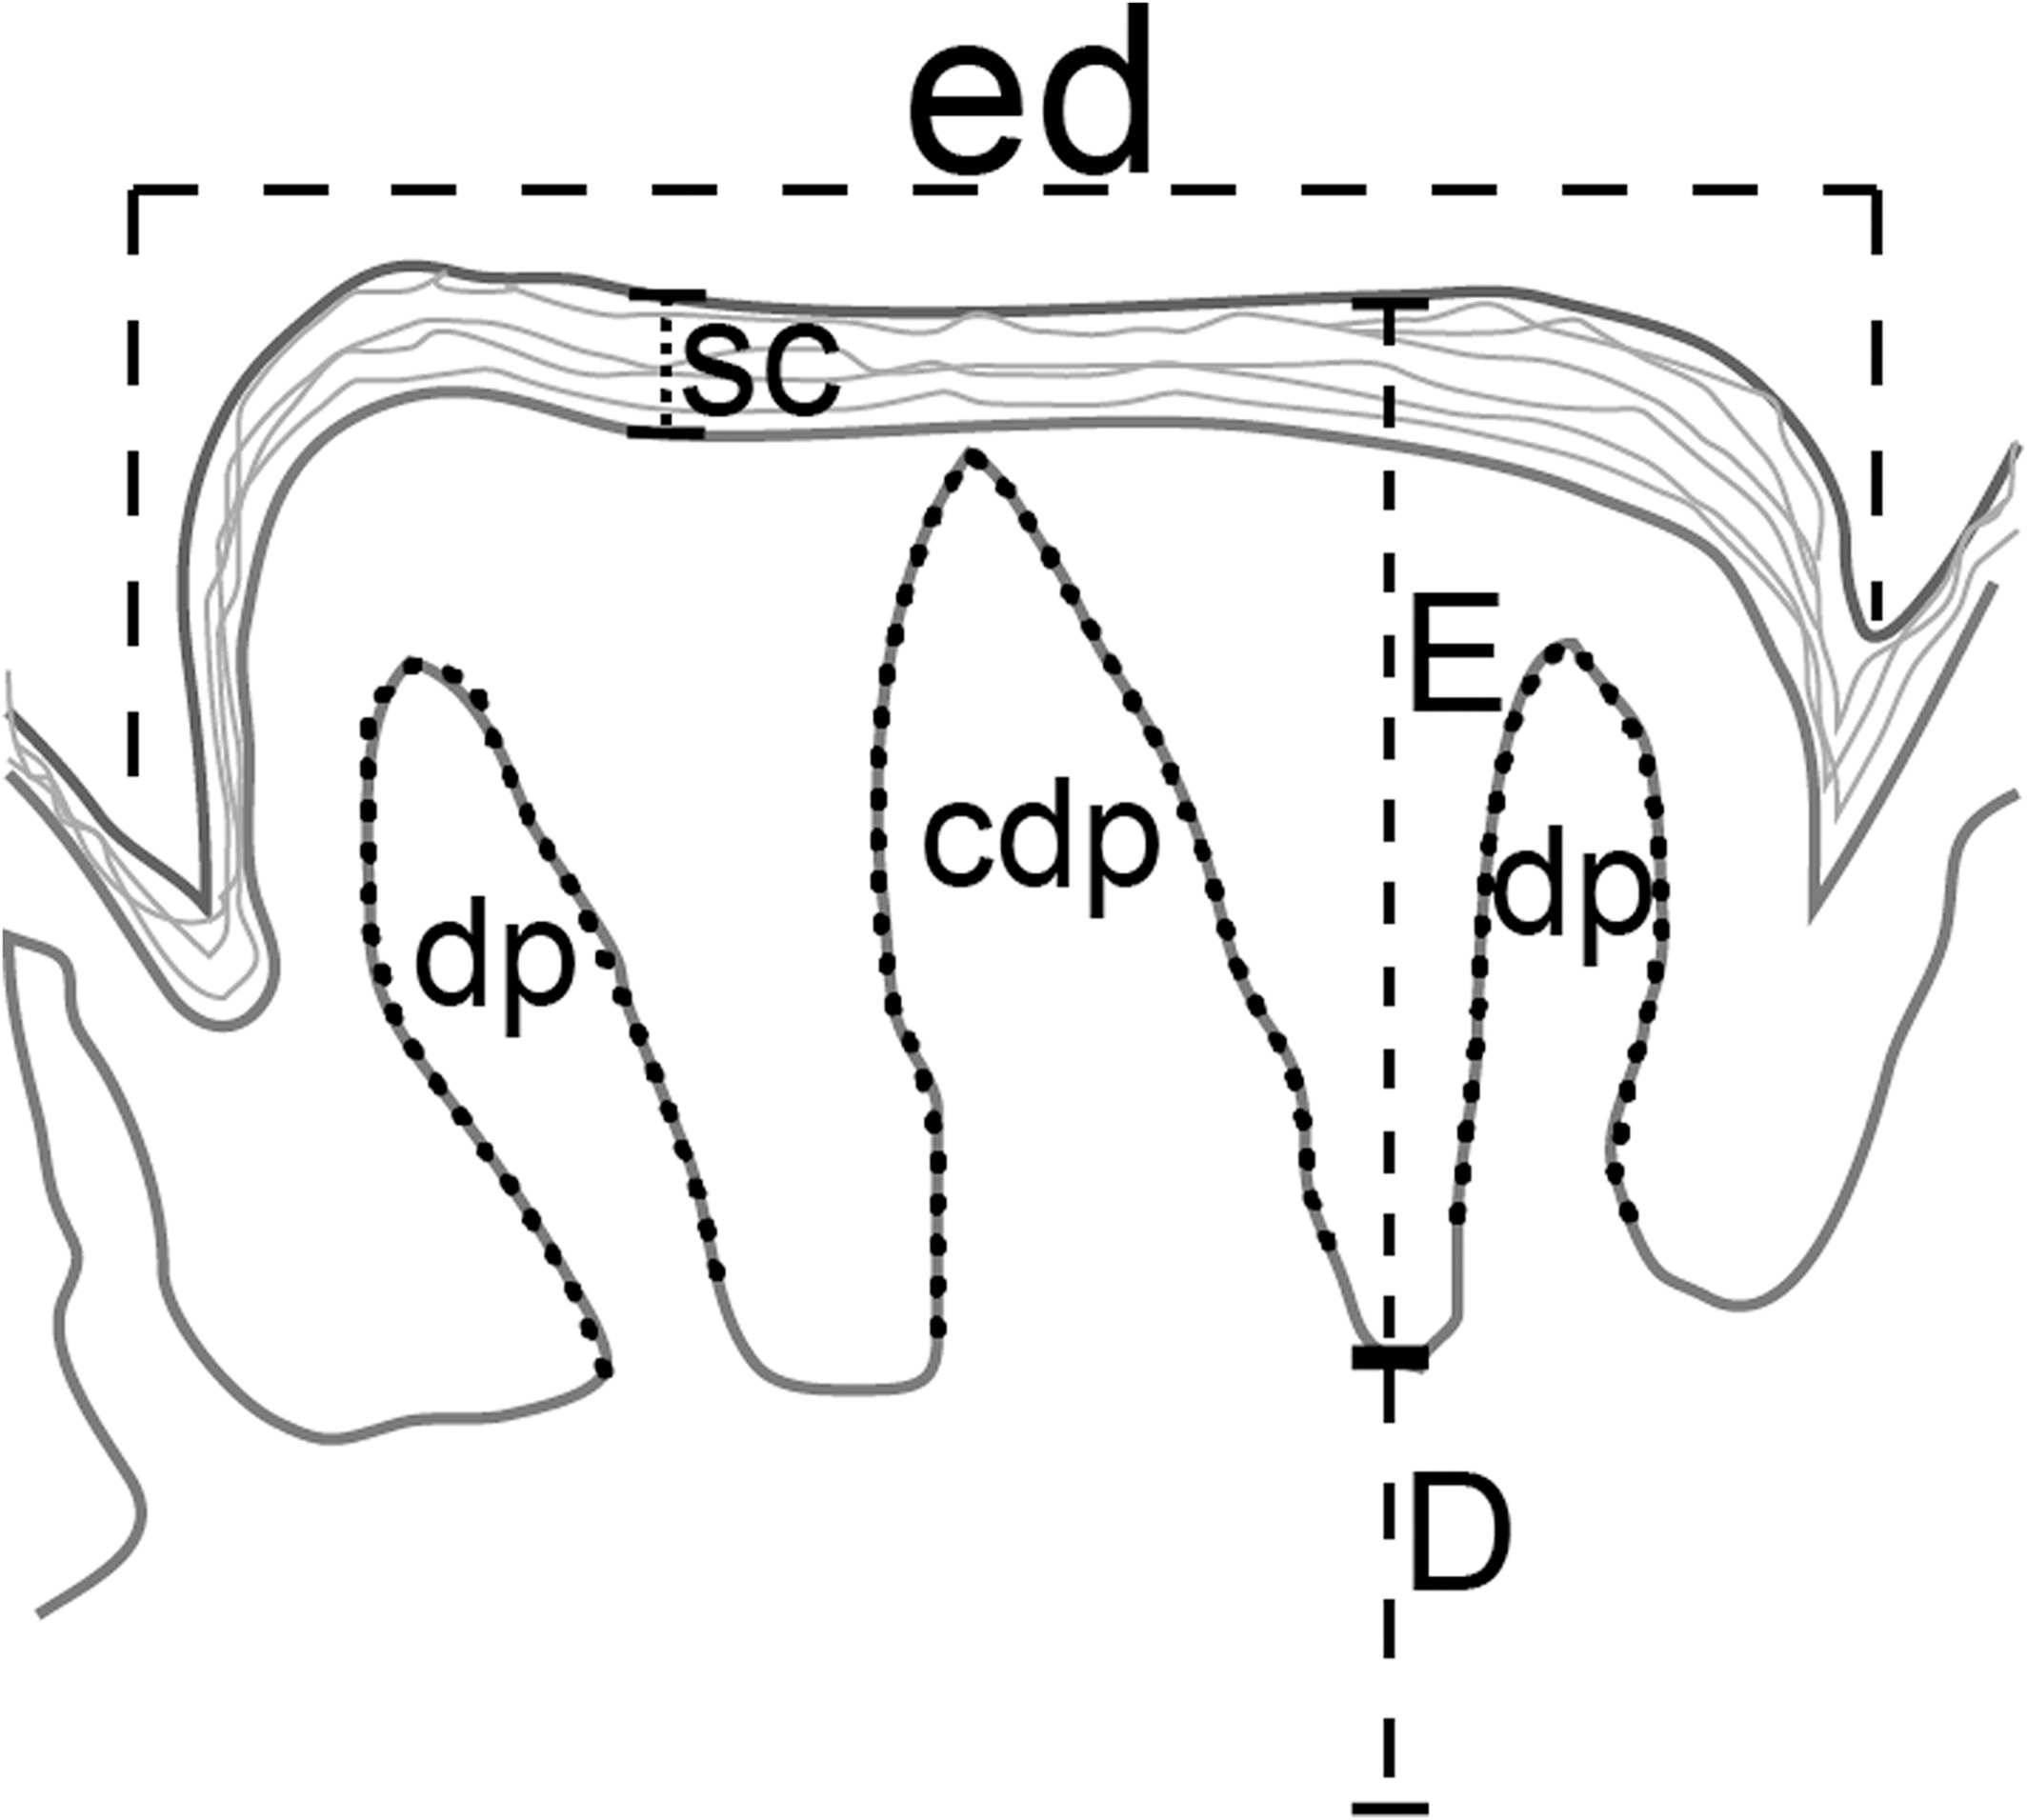
\includegraphics[width=0.5\textwidth]{obrazky/strucureRhinarium.jpg}
	\caption{Struktura rhinarium \cite{structureRhinarium}}
	\label{struktura_rhinarium}
\end{figure}


\subsection{Poškození rhinaria}
\label{poskozeni_rhinaria}
Obecně lze říci, že poškození postihující oblast rhinaria existuje značné množství a projevují se řadou možných defektů na kůži, které by mohly způsobit horší kvalitu rozpoznávání zvěře, jelikož by mohly narušit útvary na základě kterých se bude rozpoznávání v této práci provádět. V současné době se tyto poškození v databázi výrazně nevyskytují, a tak nejsou pro tuto práci zcela klíčové. Nicméně, v případě rozšíření databáze by bylo vhodné je zahrnout, aby mohly být využity v souvislosti s navazujícími pracemi. Informace ohledně těchto poškození byla poskytnuta od MVDr. Veroniky Olejníčkové, Ph.D.

Poškození oblasti rhinaria je možné rozdělit na vrozené a získané. Získané poškození může být způsobeno zraněním, infekcí nebo může být výsledkem metabolického, imunitně zprostředkovaného či neoplastického procesu. V následující části budou popsány různé typy onemocnění rozdělené dle různých kritérií:

\begin{itemize}
    \item Mezi infekční onemocnění popsané v Evropě patří Dermatophilus congolensis, Parapoxvirus of red deer a orf virus. Tyto onemocnění se projevují vznikem krust v oblasti rhinaria. Mezi další evropská onemocnění patří Papilomaviry, které se projevují vznikem kožních nádorů.
    
    \item Mezi infekční onemocnění zasahující oblast rhinaria popsané jinde ve světě patří Deerpoxvirus, Herpesvirus nebo také svrab. Deerpoxvirus se projevuje vznikem kožních poškození, krust a vředů. Herpesvirus způsobuje zánět kůže, vznik krust a vředů. V případě svrabu se poškození projevuje svěděním pří kterém si zvěř nos odře. Dalším nádorovým onemocněním popsaným ve Finsku u soba polárního je kožní lymfom.

    \item Následující onemocnění zatím nebyly popsány u parohaté zvěře nebo se neprojevily přímo v oblasti rhinaria. Virus vesicularní stomatitidy je infekce u skotu, která vede ke vzniku puchýřků v oblasti rhinaria. Capripoxvirus je původcem nodulární dermatitidy skotu, která je charakteristická vznikem kožních uzlíků u skotu (poškození se projevuje i na oblasti rhinaria). Mokokutánní pyoderma je běžné onemocnění postihující oblast rhinaria a je způsobeno bakteriemi Staphylococcus spp.. Onemocnění se projevuje vznikem krust a erozí.  Stephanofilaria okinawaensis způsubuje zánět kůže společně se vznikem krust. Plísňové onemocnění Dermatophytózy se vyskytuje u psů a projevuje vznikem papul, krust, erozí a vředů. Canidiobolomykóza je onemocnění, které bylo popsáno u psů a lamy. Onemocnění se projevuje vznikem vředů. Dalším onemocněním je Besnoitia besnoiti. Toto onemocnění bylo popsáno u soba polárního a domácích přežvýkavců v Německu, Francii a na jihu evropy. Následkem tohoto onemocnění je vasculitída se vznikem krevních sraženin a trhlin. Leishmanióza je onemocnění skotu popsané ve Švýcarsku. Poškození se projevuje jako hyperkeratóza, ulcerativní či papulární až nudulární dermatitida. Neospora caninum může jako mezihositele využít snrce nebo domácí přežvýkavce. Projevuje se na kůži rhiaria ulcerativní papulonodulární dermatitidou. Prototheca spp. je ojedinělé onemocnění postihující divoká i domácí zvířata ve světě. Projevuje se vředy, které se tvoří na místě, kde se spojují kůže a sliznice, hlavně kolem nozder a čenichu. Pyemotes tritici je roztoč, který zasahuje savce a vede ke vzniku poranění na čenichu.

    \item Dalším typem onemocnění, které by mohlo poškodit oblast rhinaria jsou metabolické a endokrinní onemocnění, které jsou popsány u domácích přežvýkavců. Mezi tato onemocnění patří dědičný nedostatek zinku, který vede ke vzniku kožních krust. Dále sem patří i Hypothyreóza, což je snížená funkce štítné žlázy a projevuje se šupinatou kůží s možných vznikem krust.

    \item Mezi autoimunitní onemocnění postihující kůži přežvýkavců patří Epidermolysis bullosa. Toto onemocnění se projevuje vznikem vředů a krust s možností sekundární infekce. Dále sem patří nemoc chladových algutininů, která vzniká postinfekčně na autoimunitním podkladě. Nemoc se zhoršuje v chladu a projevuje se modřinkami, vředy až odumíráním tkáně na končetinách, včetně nosu.

    \item Posledním typem onemocnění jsou onemocnění způsobená rostlinami a plísněmi. Mezi plísňová patří Stachybotryotoxikóza a T-2 toxikóza. Stachybotryotoxikéza je zapříčiněna toxiny plísně Stachybotrys spp., které mohou způsobit vznik vředů a odumírání tkáně na kůži domácích přežvýkavců. T-2 toxikóza je mykotoxin z plísně rodu Fusarium a spolu s jiným mykotoxinem, aflatoxinem, způsobuje především vyrážky s vředy na kůži. Mezi onemocnění způsobená rostlinami patří Fotosensitizující dermatitida a kontaktní fotodermatidída. Tyto onemocnění jsou zapříčiněna požitím nebo kontaktem s některými rostlinami a opět se projevují vznikem vyrážek a ostatních poškození. Poslední příklad těchto onemocnění vzniká požitím glykoalkaloidů solaninu a chaconinu a projevuje se vyrážkou a vředy na kůži v oblasti nosu.
\end{itemize}


\section{Shrnutí dosavadních studií a jejich výsledků}
\label{Shrnutí dosavadních studií a jejich výsledků}
Poslední dobou lze pozorovat zvýšený zájem o oblast pro rozpoznávání zvěře na základě biometrických vlastností. Některé studie se věnují rozpoznávání zvěře na základě jejich biometrických charakteristik jako jsou třeba pruhy zebry, vzory na těle gepardů a tygrů a nebo třeba stopy po zranění zanechané na těle mořských živočichů jako jsou žraloci a velryby \cite{cattle_recognition_paper}. Pro tuto práci budou ovšem nejpodstatnější výzkumy zabývající se rozpoznávání na základě vzorů na nosu. Pro rozpoznávání této konkrétní biometrické charakteristiky existuje již také řada studií. Většina se jich týká rozpoznávání dobytka u kterého je možné získat a porovnat úspěšnost jednotlivých přístupů. Tato část bude vycházet převážně z textu o dosavadních metodách pro rozpoznávání dobytku \cite{cattle_recognition_paper} a bude doplněna o shrnutí novějších studii založených na strojovém učení \cite{HOSSAIN2022138} a to včetně práci ohledně identifikace psů na základě jejich nosního vzoru \cite{psi}. 


\subsection{Systém pro rozpoznávání dobytka na základě vzoru nosu}
V této části textu se bude nacházet ilustrační obrázek toho, jak systém pro rozpoznávání dobytka může vypadat. Systém se dělí na dvě části, trénovací a testovací. V trénovací části se nasnímají fotky nosů a vyextrahují se šablony na základě rysů, ty se poté uloží do databáze. V testovací části se nasnímaný nos porovnává s ostatními nosy v databázi a snaží se najít jemu nejpodobnější. Obě tyto části se skládají z více kroků viz obrázek \ref{system_cattle}.

\newpage
\begin{figure}[h]
	\centering
	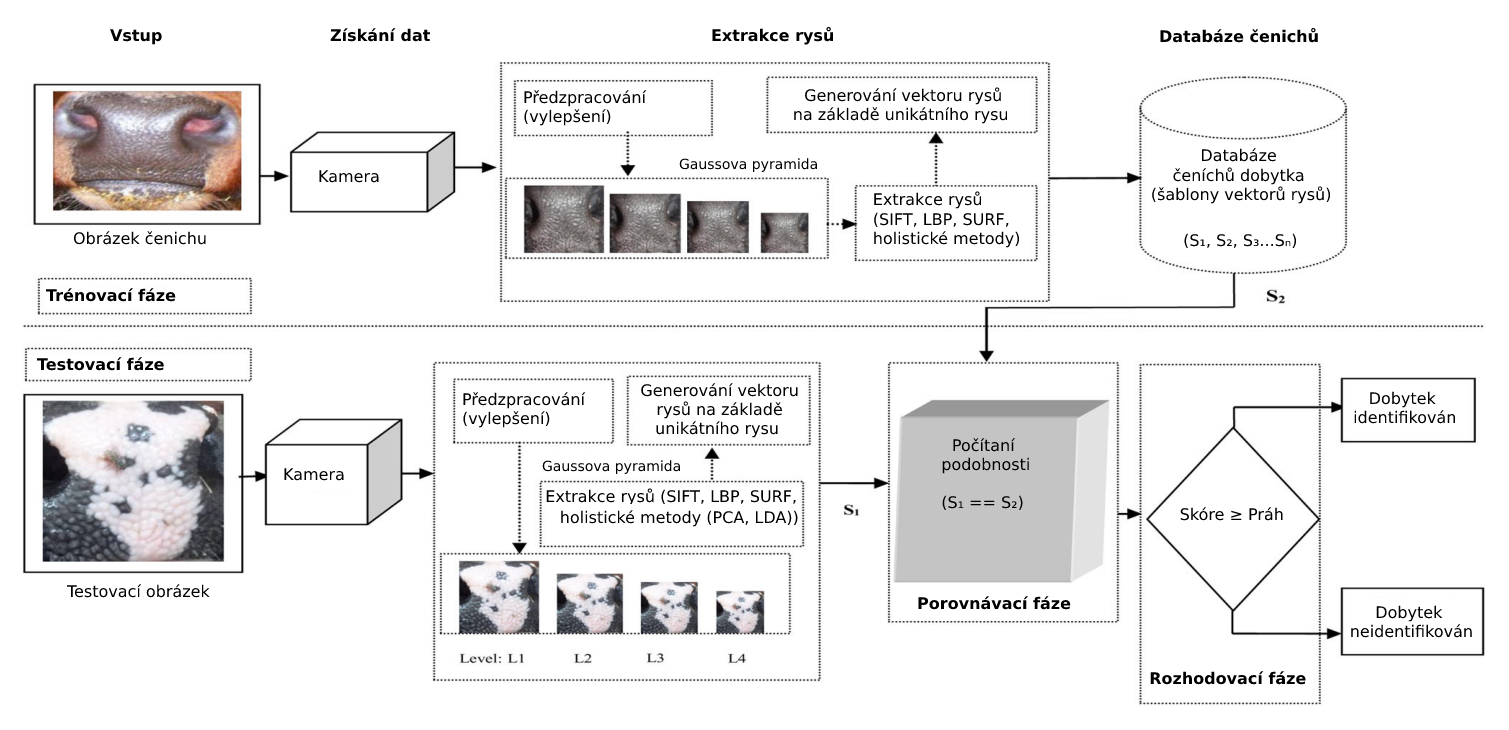
\includegraphics[width=0.8\textwidth]{obrazky/cattle_system (1).png}
	\caption{Systém pro rozpoznávání dobytku na základě vzorů nosu \cite{cattle_recognition_paper}}
	\label{system_cattle}
\end{figure}

\subsubsection{Získání dat}
Prvním krokem tohoto systému je získání dat. V tomto kroku jsou data pomocí senzoru nasnímána a poté uložena do databáze. Důležitým faktorem při pořizování těchto dat je dostatečné rozlišení a kvalita. 

\subsubsection{Předzpracování a extrakce rysů}
Dalším krokem je předzpracování a extrakce rysů. V tomto kroku se snažíme redukovat šum a ostatní chyby, které mohly vzniknout při pořizování obrázků. Redukce šumu lze dosáhnout použitím doplnopropustního filtru jako je například Gaussova pyramida viz \ref{system_cattle}. Dalším úkolem předzpracování je úprava otisku pro lepší extrakci rysů. Z tohoto důvodu se v závislosti na extrakčním algoritmu používá například skeletonizace a histogramová ekvalizace. Po předzpracování jsou z databáze extrahovány rysy, které popisují daný nos. K tomu se využijí například Scale invariant feautre transform (SIFT) \cite{6644052, NOVIYANTO201377} , Speeded up robust feature (SURF) \cite{noviyanto2012automatic}. Pro ukázku je zde uveden obrázek, který popisuje postup vytváření jednoho SIFT deskriptoru \ref{sift}.


\begin{figure}[h]
	\centering
	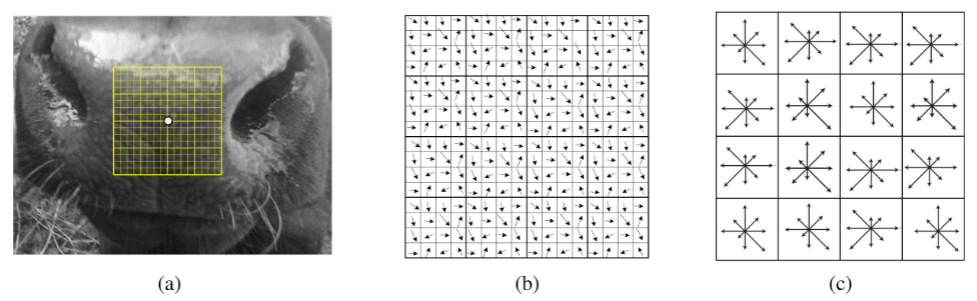
\includegraphics[width=0.8\textwidth]{obrazky/sift.png}
	\caption{Vytváření jednoho SIFT deskriptoru klíčového bodu: (a) vybraný SIFT klíčový bod z obrázku nosu, (b) výpočet gradientů pixelů v okně o velikosti 16x16, (c) výpočet deskriptoru klíčového bodu o velikosti 4x4 buněk s 8 orientacemi  \cite{cattle_recognition_paper}}
	\label{sift}
\end{figure}


\subsubsection{Generování šablon}
Následuje generování šablon reprezentující původní vzor nosu na základě extrahovaných rysů. Rysy vybrané pro reprezentaci nosu jsou vybrány na základě jejich unikátnosti. Vygenerovaná šablona je poté uložena do databáze.

\subsubsection{Porovnávání}
Poté nastane porovnávací fáze. V této fázi se rysy extrahované zvolenou metodou  porovnávají s šablonou z databáze. Tím vznikne hodnota podobnosti dvou šablon, která v případě že dosahuje určitého prahu způsobí, že se nosy prohlásí za shodné. Pro ukázku je na obrázku \ref{sift_match} uvedeno porovnávání na základě metody SIFT.

\begin{figure}[h]
	\centering
	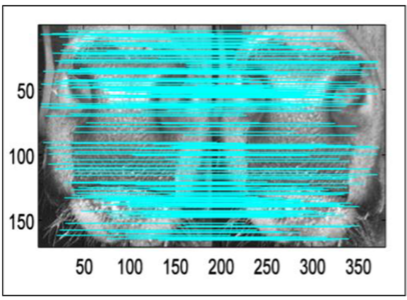
\includegraphics[width=0.6\textwidth]{obrazky/sift_match.png}
	\caption{Porovnávání fotografií nosu na základě metody SIFT \cite{cattle_recognition_paper}}
	\label{sift_match}
\end{figure}

\subsection{Konkrétní přístupy a jejich výsledky}

První systém pro identifikaci dobytka na základě nosu byl v roce 2002 navržen v práci \textit{Identification of beef cattle by analyzing images of their muzzle patterns lifted on paper} \cite{minagawa2002identification}. Systém pro rozpoznávání využíval pixely, které spojovaly drážky nacházející se na nosu. Nalezení těchto bodů bylo dosáhnuto pomocí řady technik pro zpracování obrazu jako filtrování, binarizace a skeletonizace obrazu. Tento sytém jako vstup využíval naskenované otisky nosů zanechané na papíře. Výsledkem této práce byl systém, který dokázal rozpoznat dobytek s 30\% úspěšností.

Další systém pro rozpoznávání zvěře pomocí počítačového vidění byl od autorů Ary Noviyanto a Aniati Murni Arymurthy \cite{NOVIYANTO201377}. Tento systém využíval metody SIFT pro získání konkrétních rysů. Výsledný systém vykazoval přesnost 0.0167 equal error rate (EER) \footnote{EER se používá jako ukazatel přesnosti biometrických systémů, přičemž čím víc se hodnota blíží k nule, tím lépe. Konkrétně se jedná o hodnotu, která vyjadřuje míru chybně pozitivních a chybně negativních výsledků.}. Navíc autoři vylepšili tuto metodu pomocí orientací jednotlivých rysů. Tímto se eliminovali některé milné shody. Výsledkem toho byl systém, který vykazoval přesnost 0.0028 EER, což je lepší než byl původní navržený způsob. 

V knize \textit{2013 Federated Conference on Computer Science and Information Systems} \cite{6644052} byl navržen systém, který využíval metody SIFT pro extrakci rysů a následné hledání shody. Pro větší robustnost systému byl SIFT skombinován s Random sample consensus (RANSAC). Z důvodu malé databáze obrázků, byly na obrázky aplikovány různé rozmazání, rotace a řezy, aby se otestovala robustnost tohoto systému. Díky kombinaci SIFT a RANSAC výsledný systém dosahoval přesnosti 93,3\%, což bylo více než předešlé navržené systémy.

V roce 2013 byl v časopise \textit{Transactions of the ASABE} navržen systém, který pro zpracování digitálních obrazů využíval Principal Component Analysis (PCA) a Euklidovské metriky pro klasifikaci. Hlavním elementem pro zvyšování úspěšnosti rozpoznávání tohoto přístupu bylo zvyšování počtu obrázků při trénování. 

V knize \textit{Proceedings of the 3rd European conference of computer science, ECCS} \cite{noviyanto2012automatic} byly rysy extrahovány pomocí metody SURF. Na základě provedených experimentů se dokázalo, že tento systém zvládne překonat předchozí výzkumy, které extrahovali rysy pomocí vlastních vektorů. S dostatečným počtem vstupních dat se ukázalo, že SURF může mít více než 90\% přesnost. Dále zkoumali metodu Upright-SURF (U-SURF), která dokázala překonat i dříve zmíněnou metodu SURF, ale pouze za předpokladu, že data byla orientačně normalizována.

Další navržený systém byl popsán v časopise \textit{International Journal of Image Mining} \cite{doi:10.1504/IJIM.2015.070022}. V tomto případě jsou vstupní obrazy prvně předzpracovány. K tomu autor využívá histogramové ekvalizace a filtrování pro redukci šumu. Následuje tzv. box-counting algorithm (BCA) pro detekci rysů daného nosu. Aby autor dosáhl lepších výsledků využil multiclass support vector machines (MSVM) pro klasifikaci. 

Autoři v knize \textit{Advanced Machine Learning Technologies and Applications} \cite{10.1007/978-3-319-13461-1_23} pro extrakci rysů využili Gáborovy rysy a pro identifikaci využili strojové učení. Konkrétně se jednalo o support vector machines (SVM) s různými jádry. Na základě testování se ukázalo, že Gaussovo jádro vykazovalo nejlepší výsledky. Dále podobný tým autorů navrhl systém, který extrahoval rysy pomocí LBP \cite{10.1007/978-3-319-08156-4_22}. V tomto výzkumu zkoušeli využít různých identifikačních metod, konkrétně tedy neural network (NN), k-nearest neighbour (K-NN), SVM a naivního bayese. 

Výzkumů na toto téma je značné množství, ovšem z těch novějších lze vyvodit, že trend rozpoznávání dobytka na základě nosu spěje směrem ke strojovému a hlubokému učení. Jelikož se ovšem kategorie výzkumů, které využívají hlubokého učení, zaměřuje převážně na identifikaci dobytka na základě odlišných biometrických charakteristik než je fotografie nosu (například vzor srsti), tak zde nebudou brány v potaz. Mezi nejčastěji používané modely strojového učení pro identifikaci dobytka patří SVM, K-NN a artificial neural network (ANN) \cite{HOSSAIN2022138}. Nejčastějšími metodami pro extrakci samotných rysů patří convolutional neural network (CNN), local binary pattern (LBP), SURF, SIFT, Inception a Visual Geometry Group (VGG) \cite{HOSSAIN2022138}. Pro přehlednost zde bude uvedena tabulka, která obsahuje studie týkající se rozpoznávání dobytka pomocí metod strojového učení \ref{tabulka_ML}. Významy zkratek v tabulce, které doposud nebyly zmíněny jsou následující:

\newpage
\begin{itemize}
        \item F = F-skóre \footnote{F-skóre je metrika pro vyhodnocení kvality klasifikace modelu strojového učení, což znamená rozdělení do dvou kategorií, například pozitivní a negativní. F-skóre se vypočítává se na základě přesnosti a úplnosti. Přesnost je definována jako počet správně klasifikovaných jako pozitivních zatímco úplnost vyjadřuje, kolik z celkového počtu pozitivních bylo klasifikováno jako pozitivní. F-skóre se poté vypočítá následovně $ \text{F-skóre} = \frac{2 * (\text{přesnost} * \text{úplnost})}{\text{přesnost} + \text{úplnost}} $.}
        \item GSRC = Group sparsity residual constraint
        \item FLPP = Fuzzy linear preserving projections
        \item WLD = Weber’s native descriptor
\end{itemize}

\begin{table}[h]
    \begin{tabular}{l|l|c|l|l}
      \multicolumn{1}{c|}{Reference} & Nejlepší model & \multicolumn{1}{|p{2cm}|}{\centering Velikost \\ databáze} & \multicolumn{1}{|p{2cm}|}{\centering Metoda pro \\ extrakci} & Úspěšnost \\ \hline
       Kusakunniran \cite{8693161} & SVM & 217 & LBP & 100\%     \\ \hline
       Awad \cite{app9224914} & SVM & 105 & SURF & 93\%     \\ \hline
       Kumar \cite{Kumar2018} & GSRC & 5000 & LBP & 93,87\%   \\ \hline
       Kumar \cite{Kumar2017} & ANN & 5000 & LBP & 96,74\%     \\ \hline
       Kumar \cite{https://doi.org/10.1049/iet-ipr.2016.0799} & K-NN & 5000 & SURF &  93,87\%    \\ \hline
       Kumar \cite{Kumar2017a} & SVM & 5000 & FLPP & 96,87\%     \\ \hline
       Gaber \cite{GABER201655} & AdaBoost & 217 & WLD &  98,9\%    \\ \hline
       Zaorálek \cite{10.1007/978-3-319-29504-6_11} & SVM & 322 & SVD & 75F  \\ \hline
       Ahmed \cite{7312056} & SVM & 217 & SURF & 100\%     \\ \hline
       Tharwat \cite{10.1007/978-3-319-13461-1_23} & SVM & 217 & Gáborův filtr & 99,5\%     \\ \hline
       Tharwat \cite{10.1007/978-3-319-08156-4_22} & SVM & 217 & LBP & 99,5\%     \\ \hline
       El Henawy \cite{el2017muzzle} & ANN & 1060 & BCA & 99,18\% 
    \end{tabular}
    \caption{Tabulka shrnující přístupy strojového učení pro rozpoznávání dobytka na základě vzoru nosu \cite{HOSSAIN2022138}}
    \label{tabulka_ML}
\end{table}


V roce 2020 byl navrhnut podobný systém pro identifikaci psů \cite{psi}. Ten pro předzpracování využíval histogramové ekvalizace a změny velikosti obrazu. Pro extrakci rysů z otisku bylo využito několika metod u kterých bylo provedeno následné srovnání úspěšnosti extrakce. Těmito metody byly konkrétně SIFT, SURF, Binary Robust Invariant Scalable Keypoints (BRISK) a oriented FAST and rotated BRIEF (ORB). Porovnávání nalezených rysů se dělalo dvěma způsoby. V případě SIFT a SURF byl použit Fast library for approximate nearest neighbors (FLANN). V případě BRISK a ORB byla použita hammingova vzdálenost. Testování probíhalo na databázi o velikosti 990 obrázků, které byly vytvořeny deformacemi, rotacemi a změnami osvětlení u původních 55 obrázků. Těchto 55 obrázků nosů patřilo 11 různým psům. Z výsledků vyplynulo, že nejlépe si vedla metoda ORB, která měla 0,35 EER.


\newpage
\section{Identifikace na základě otisku prstu}
\label{Identifikace na základě otisku prstu}
%TODO napsat omacku ohledne identifikace

Následující text se bude věnovat celému procesu rozpoznávání otisku prstu. První část ohledně předzpracování otisku je převzata z \cite{otiskyPrstu, otiskyPrstu2}, druhá část ohledně extrakce markantů je z \cite{jain1999multichannel}. Poslední část, kde je stručně sepsáno rozpoznávání a klasifikace otisku je převzata z \cite{otiskyPrstu}. Na následujícím obrázku lze vidět jak celý systém rozpoznávání otisků prstů může vypadat \ref{finger_preprocessing_system}.

\begin{figure}[h]
	\centering
	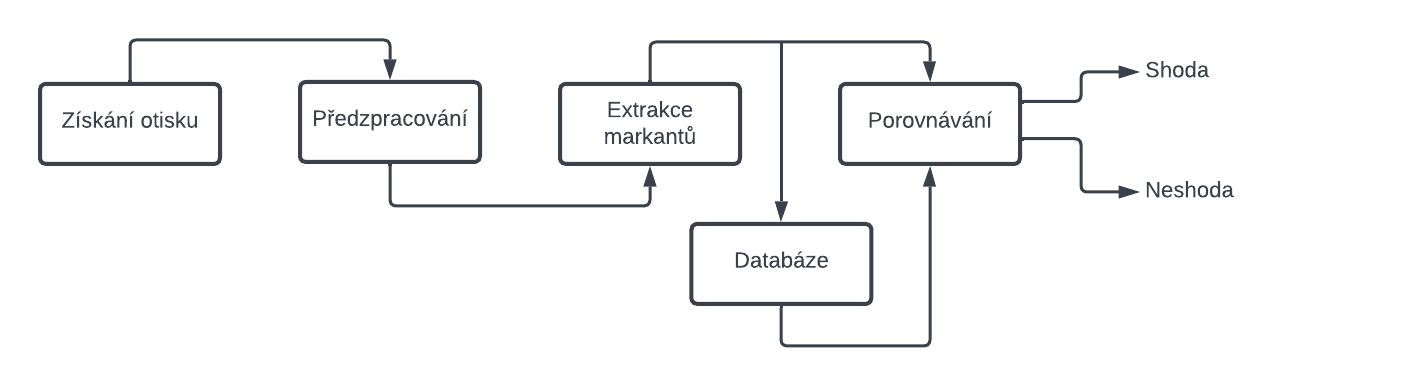
\includegraphics[width=0.9\textwidth]{obrazky/finger_proces.png}
	\caption{Systém rozpoznávání otisku prstu \cite{fingerprintOverview}}
	\label{finger_preprocessing_system}
\end{figure}


\subsection{Otisk prstu}
\label{Otisk prstu}
Otisk prstu je jedinečný a nezaměnitelný vzor tvořený papilárními liniemi, který vzniká kontaktem pokožky prstu s jiným povrchem. Na otisku prstu se nachází tzv. papilární linie, což jsou výběžky kůže, na základě kterých se celé rozpoznávání řídí. Tyto linie vytvářejí různé dráhy a křivky, které jsou specifické pro každého jednotlivce a tudíž nejsou stejné u žádných dvou osob. Otisk prstu je tvořen hřebeny a brázdami. Hřeben je vystouplá část kůže tvořící papilární linie zatímco brázda je naopak prohlubeň mezi hřebeny. Zde lze pozorovat podobnost s rhinariem, kde jsou polygony ohraničené rýhami. Na otiscích uvedených níže budou hřebeny reprezentovány černou barvou a brázdy naopak barvou bílou.


\subsection{Předzpracování otisku prstu}
\label{Předzpracování otisku prstu}

Předzpracování slouží v případě otisku prstu k vylepšení kvality nasnímaného otisku. Zabývá se opravou obnovitelných regionů a odstraněním regionů neobnovitelných. Dělí se do kategorií podle velikosti oblastí na základě aplikace algoritmu použitého pro opravu. Díky těmto opravám jsme schopni v otisku odstranit chyby, které by mohly způsobit, že navazující algoritmus pro extrakci markantů nebude pracovat dostatečně dobře. Na následujícím obrázku je uvedena ukázka, jak předzpracování může vypadat jako sekvence po sobě jdoucích operací \ref{finger_preprocessing}.


\newpage
\begin{figure}[h]
	\centering
	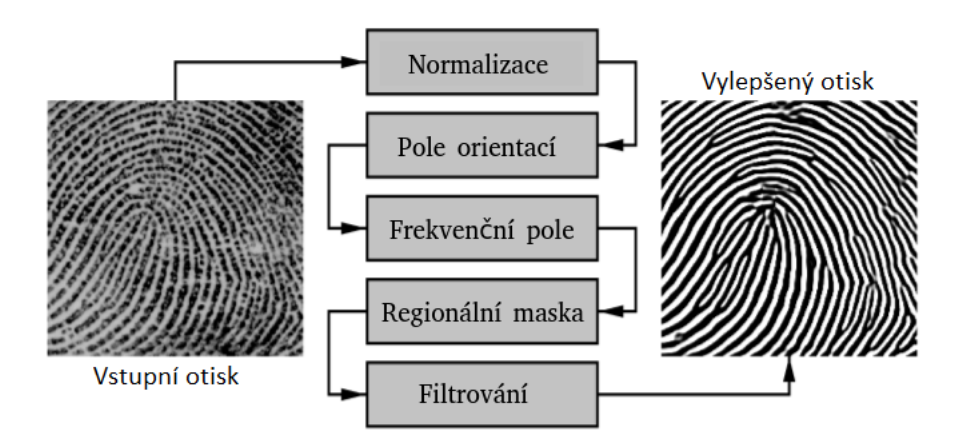
\includegraphics[width=1\textwidth]{obrazky/preProcessing.png}
	\caption{Předzpracování otisku prstu \cite{otiskyPrstu}}
	\label{finger_preprocessing}
\end{figure}

\subsubsection{Normalizace}
Prvním krokem předzpracování je normalizace. Během normalizace se zmenšují rozdíly intenzit pixelů mezi hřebeny a brázdami. Toho algoritmus vypočítá novou hodnotu pixelu na základě aktuální hodnoty pixelu a statických ukazatelů obrazu jako je průměr a rozptyl. Díky tomu nebude následující algoritmus pro rozpoznávání orientací rušen šumem a dalšími nevyžádanými prvky jako je například různý kontrast mezi hřebeny a brázdami, který může být způsoben rozdílnou sílou přítlaku \cite{otiskyPrstu2}.

\subsubsection{Pole orientací}
Pole orientací je způsob reprezentace směru papilárních linií v obrazu rozděleném na nepřekrývající se bloky. Jeden tento blok si můžeme představit jako vyříznutou část vstupního obrázku například o velikosti čtverce. Algoritmus pro určení orientací využívá vlastnosti, že směr linie v bloku jsou ortogonální vůči jejímu gradientu.

\subsubsection{Frekvenční pole}
Frekvenční pole spolu s polem orientací slouží jako vstup pro finální vylepšení otisku pomocí Gáborova filtru. Toto pole, stejně jako je tomu u pole orientací, obsahuje jednotlivé bloky obrazu. Tentokrát je ovšem blok reprezentován sinusovou funkcí, jejíž průběh kopíruje výskyt papilárních linií se směrnicí kolmou k orientaci linií v daném bloku. Tento postup se aplikuje pouze v případech, kdy se v bloku nenachází žádný markant nebo singulární bod \cite{otiskyPrstu}.

\subsubsection{Regionální maska}
Regionální maska je reprezentace otisku po regionech, kde každý jeden region má přidělen hodnotu na základě jeho kvality. Ta se dělí do těchto tří typů:


\begin{itemize}
    \item Dobře specifikovaný region
    \item Obnovitelný poškozený region
    \item Neobnovitelný poškozený region
\end{itemize}

První dvě kategorie lze sumarizovat jako kategorie obnovitelné a tu poslední jako neobnovitelnou. Pro určení do které kategorie daný region spadá se využívá řady kritérií. Po určení kategorie všech regionů, lze stanovit poměr obnovitelných regionů vůči regionům neobnovitelným. Tento poměr představuje úroveň kvality. V případě potřeby se tímto způsobem dá rozlišit kvalitní a nedostatečně kvalitní vstupní otisk.

\subsubsection{Filtrování}
Posledním krokem v procesu předzpracování je filtrování. V této části se využije vypočítaných frekvencí a orientací v blocích, které poslouží jako vstupy do Gáborova filtru. Tento filtr následně po blocích odstraňuje šum a zároveň neupravuje hřebeny a brázdy. Výsledek po filtrování lze vidět na obrázku \ref{finger_preprocessing}.


\subsection{Extrakce markantů}
\label{Extrakce markantů}

Extrakce markantů je proces, jehož vstupem je předzpracovaný obraz. Cílem tohoto procesu je lokalizace a zakódování důležitých bodů (markantů), které budou blíže popsány v části o rozpoznávání a klasifikace otisku prstu \cite{fingerprintOverview}. Kromě polohy markantu se většinou ještě uchovává jejich typ a směr. Existuje spousta metod pro extrakci markantů. Některé z nich využívají přímo šedotónového obrazu, z kterého za pomocí Gáborova filtru extrahují markanty \cite{ZHAO20071270}. Většinou se ovšem na vylepšený obraz aplikuje následující postup.

\subsubsection{Binarizace}
Prvním krokem je binarizace, což je převod šedotónového obrazu do pouze dvou úrovní (černá a bílá). Tento proces se provádí za pomocí hodnoty prahu, která určuje jestli se aktuální hodnota pixelu změní na bílou a nebo černou. 

\subsubsection{Skeletonizace}
Následně se provádí skeletonizace obrazu. Tento proces převádí binarizovaný obraz na jeho kostru. Tuto kostru lze chápat jako výsledek morfologických operací (eroze), které postupně odstraňují vnější část linií až do doby, kdy už linie nejde více ztenčit.

Následně se na skeletonizavaný otisk aplikuje algoritmus pro vyhledávání markantů. Výsledek extrakce markantů bude vyznačen na následujícím obrázku \ref{finger_preprocessing2}.

\newpage
\begin{figure}[h]
	\centering
	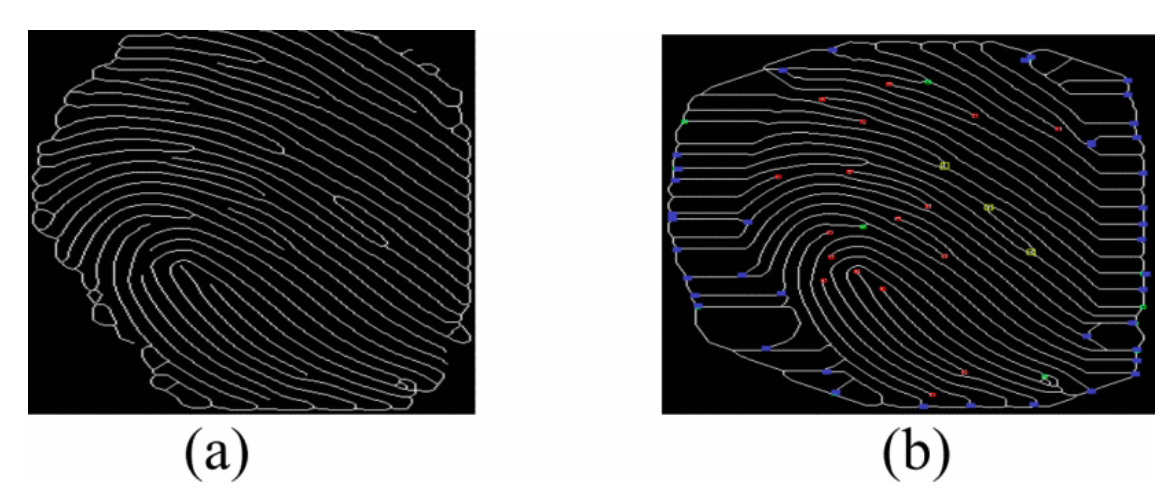
\includegraphics[width=0.8\textwidth]{obrazky/finger_markant.png}
	\caption{ (a) skeletonizovaný otisk, (b) markanty \cite{fingerprintOverview}}
	\label{finger_preprocessing2}
\end{figure}


\subsection{Porovnávání a klasifikace otisku prstu}
\label{Porovnávání a klasifikace otisku prstu}
Následující text bude rozčleněn do dvou částí, kde se první část bude zabývat procesem porovnávání otisků prstů a druhá bude o klasifikaci otisku prstu.


\subsubsection{Porovávání otisků prsů}
Porovnávání otisku prstu využívá získané množiny markantů z předchozího kroku. Typickým příkladem porovnávání na základě množiny markantů je Hongova a Rathova metoda \cite{FITMT25007}. V prvním kroku se porovnávané otisky zarovnají (typicky podle singulárního bodu typu jádro) a následně se provede porovnávání markantů. Během toho se porovnávají dříve zjištěné vlastnosti jednotlivých markantů jako je jejich pozice, směr a typ. V případě, že si je vstupní otisk dostatečně podobný s otiskem v databázi, jsou otisky prohlášeny za shodné. Míra této shody závisí na nastavené hranici. V případě, že je tato hranice nastavena jako příliš malá, bude pravděpodobněji docházet ke shodě dvou různých otisků. Naopak v případě, že hranice je nastavena příliš vysoko, mohou i drobné nečistoty či jiné odchylky způsobit, že systém otisky označí za neshodné.

\textbf{Markanty} jsou specifické útvary tvořené papilárními liniemi a mohou se dělit do různých typů na základě útvaru, který tvoří papilární linie. Na základě těchto bodů lze unikátně reprezentovat jakýkoli otisk prstu. Pro tuto práci budou markanty obzlášť stěžejní, jelikož se pomocí nich bude popisovat nos zvěře viz \ref{Fotografie nosu}. Pro ukázku je na obrázku \ref{markanty_prst} uvedeno pár základních typů markantů u otisku prstu.



\begin{figure}[h]
	\centering
	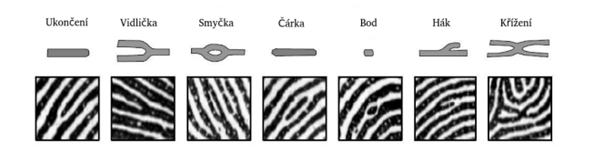
\includegraphics[width=0.8\textwidth]{obrazky/markanty.png}
	\caption{Základní typy markantů \cite{otiskyPrstu}}
	\label{markanty_prst}
\end{figure}

\subsubsection{Klasifikace otisků prsů}
Klasifikace otisků se provádí na základě počtu a pozic singulárních bodů, což jsou důležité globální body. Tyto body se dělí na delty a jádra. Jádro je definováno jako nejvyšší bod nejvnitřnější smyčky a delta je středem trojúhelníkových oblastí. Na obrázku \ref{singularni_body} jsou zobrazeny základní vzory papilárních linií. Tyto vzory se od sebe liší pozicemi a počtem singulárních bodů. Klasifikace otisků má za cíl zvýšit efektivitu srovnávacího algoritmu tím, že umožňuje porovnávat otisky, které spadají do stejné kategorie.



\begin{figure}[h]
	\centering
	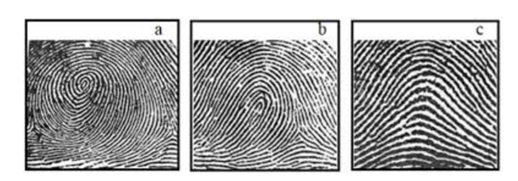
\includegraphics[width=0.8\textwidth]{obrazky/otisky.png}
	\caption{Základní vzory papilárních linií, (a) spirála, (b) smyčka, (c) oblouk \cite{otiskyPrstu}}
	\label{singularni_body}
\end{figure}


\chapter{Předběžný návrh implementace}
\label{predbezny_navrh}
V první části této kapitoly jsou uvedeny některé základní pojmy a algoritmy, které je nutné znát pro porozumění návrhu a implementaci systému pro rozpoznávání zvěře. Druhá část popisuje samotný návrh tohoto systému. Kromě popisu jednotlivých částí, ze kterých se systém skládá, jsou zde uvedeny také krátké náčrtky myšlenek, které nebyly použity v konečné verzi implementace, včetně vysvětlení důvodů, proč od nich bylo opuštěno.

\section{Navržené algoritmy}
V této podkapitole budou uvedeny všechny pojmy a algoritmy potřebné pro pochopení návrhu implementace.


\subsection{Bilaterální filtr}
\label{bilateral_chapter}


Filtr je založen na Gaussově filtru, který pro filtrování využívá konvuluce \footnote{Konvoluce je matematická operace, která spojuje dvě funkce reprezentující obraz a jádro. Jádro lze chápat jako tabulku, která obsahuje váhy určené na základě koeficientů filtru. Konvoluce se provádí tak, že se jádro posouvá přes obraz a v každém bodě se vypočítá vážený průměr hodnot v okolí zpracovávaného bodu. Tento průměr poté představuje novou hodnotu pixelu.} okolních pixelů s 2D Gaussovým jádrem. Problémem tohoto filtru je, že pro výpočet nové intenzity pixelu bere v potaz pouze jeho okolí, což může zapříčinit, že na místech kde se nachází velké rozdíly intenzit pixelů (hrany) se tyto rozdíly vyhladí. Z tohoto důvodu se aplikuje ještě druhý Gaussův filtr, který se dívá na intenzity pixelů v okolí. Ten způsobí, že při aplikaci filtru budou významnější pixely, které mají podobnější intenzitu. Díky tomu bilaterální filtr zachovává rozdíly intenzit pixelů v místech, kde se nachází hrany a zároveň vyhlazuje obraz a odstraňuje šum. Ukázka vytvoření bilaterálního jádra na základě původního obrazu a Gaussova jádra se nachází na následujícím obrázku \ref{ukazka_jader}.

\newpage
\begin{figure}[h]
	\centering
	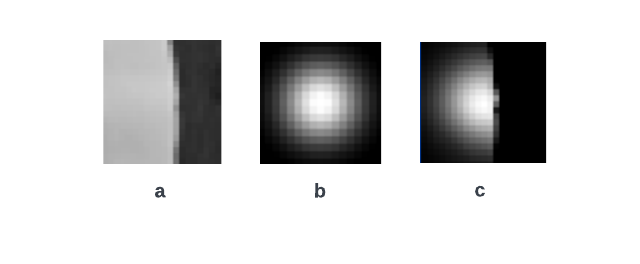
\includegraphics[width=0.8\textwidth]{obrazky/bilateral_kernel.png}
	\caption{Aplikované jádra při filtraci. (a) obraz s hranou, (b) Gaussovo jádro, (c) bilaterální jádro \cite{bilateral_kernel}}
	\label{ukazka_jader}
\end{figure}


Dále zde bude rozepsán vzoreček, který bilaterální filtr používá a to včetně popisku k jednotlivým částem, z kterých se skládá \ref{bilateral_equ} \ref{bilateral_equ2}.

\begin{equation}
    BF[I]_{p} = \frac{1}{W_{p}} \sum_{q \in S} G_{o_{s}} (\| p - q \|) G_{o_{r}} (|I_{p} - I_{q}|) I_{q}
    \label{bilateral_equ}
\end{equation}
kde 
\begin{equation}
    W_{p} =  \sum_{q \in S} G_{o_{s}} (\| p - q \|) G_{o_{r}} (|I_{p} - I_{q}|)
    \label{bilateral_equ2}
\end{equation}

    
\begin{itemize}
    \item $BF[I]_{p}$ - výsledná intenzita pixelu p
    \item $\frac{1}{W_{p}}$ - normalizační část, zajišťuje, že součet vah v okolí bude dohromady dávat 1 
    \item $G_{o_{s}} (\| p - q \|)$ - váhy podle vzdálenosti od daného pixelu
    \item $o_{s}$ - uvažované okolí pixelu
    \item $G_{o_{r}} (|I_{p} - I_{q}|)$ - váhy podle rozdílů intenzit pixelů
    \item $o_{r}$ - minimální amplituda hrany, čím víc se blíží nekonečnu, tím víc se filtr podobá Gaussovu filtru
    \item $I_{q}$ - intenzita pixelu q
\end{itemize}


\subsection{Ekvalizace histogramu}
\label{ekvalizace_chapter}

\textbf{Ekvalizace histogramu} je globální metoda, která slouží k zlepšení kontrastu a jasnosti obrazu. Metoda je založena na analýze histogramu, který obsahuje rozložení intenzit pixelů v obraze. Hlavním úkolem histogramové ekvalizace je změnit rozložení intenzit pixelů v obraze tak, aby byly rovnoměrněji rozprostřeny přes celý rozsah intenzit šedi \ref{histo_equ}. Toho se dosáhne tak, že se nejprve normalizuje histogram, aby všechny jeho hodnoty spadaly do rozsahu 0 až 1. Tento krok se dělá tak, že každý sloupec histogramu bude reprezentován pravděpodobností, že při výběru náhodného pixelu obrazu, bude tento pixel spadat do daného sloupce. Následně se vypočte kumulativní distribuční funkce (CDF) \footnote{Kumulativní distribuční funkce je neklesající funkce, která určuje pravděpodobnost, že při výběru náhodné proměnné bude tato proměnná menší než zadaná hodnota.} histogramu. Nakonec se pomocí inverzní distribuční funkce vytvoří nová intenzita pro všechny pixely. Nevýhodami této metody jsou zvýraznění šumu v obraze a ztráta detailu v příliš tmavých nebo světlých oblastech. 

\begin{figure}[h]
	\centering
	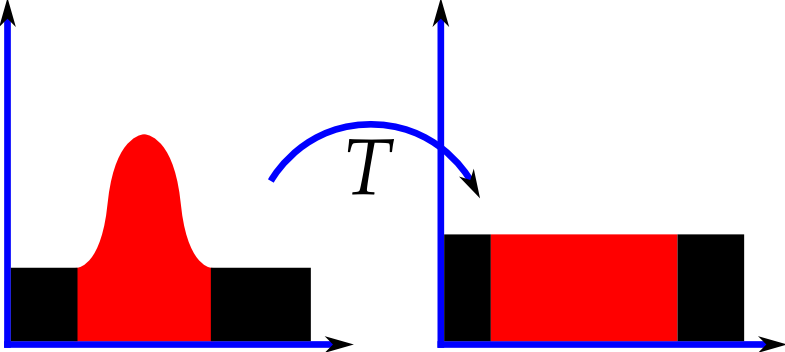
\includegraphics[width=0.6\textwidth]{obrazky/Histogram.png}
	\caption{Vyrovnání histogramu \cite{histo_equ}}
	\label{histo_equ}
\end{figure}


Vylepšením této metody je tzv. \textbf{adaptivní histogramová ekvalizace} (AHE), která rozděluje obraz do bloků. Pro každý z těchto bloků se vypočítá histogram a následně se provede jeho vyrovnání. To umožňuje adaptivní vyrovnání histogramu, které je přizpůsobeno lokálnímu kontrastu a jasu v daném bloku. Po vyrovnání dojde k vyhlazení přechodů mezi jednotlivými bloky pomocí bilineární a lineární interpolace. Tento krok se dělá z důvodu, aby se zamezilo viditelným přechodům mezi jednotlivými bloky. Tato metoda ovšem také není ideální, jelikož může zesílit šum v částech obrazu s podobnými intenzitami pixelů (tzv. bílý šum).

Z toho důvodu existuje vylepšení této metody nazývající se \textbf{kontrastně limitovaná adaptivní histogramová ekvalizace} (CLAHE). Ta před výpočtem nové hodnoty pixelů pomocí „clip-limit“ ořezává sloupce histogramu, které přesahují zvolenou hranici a rovnoměrně je rozdistribuuje mezi ostatní sloupce viz \ref{clip-limit}. Díky tomu se zachová původní četnost intenzit pixelů a zároveň se zamezí zesílení šumu.

\begin{figure}[h]
	\centering
	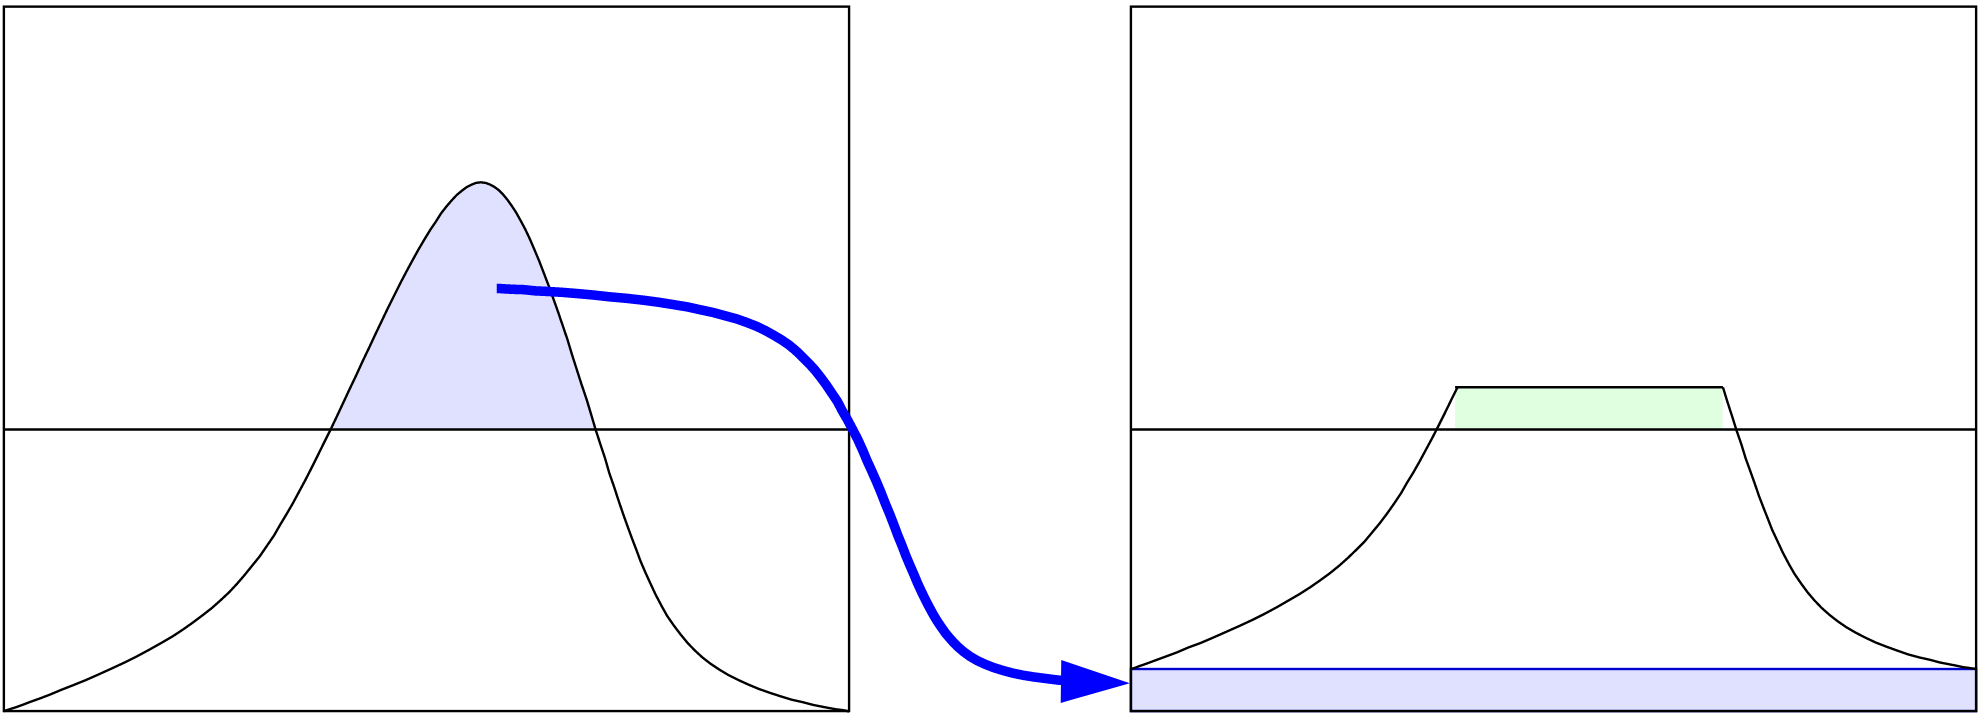
\includegraphics[width=0.6\textwidth]{obrazky/clip-limit.png}
	\caption{Aplikace clip-limit na historgram \cite{clip-limit}}
	\label{clip-limit}
\end{figure}

Na následujícím obrázku se nachází ukázka rozdílu mezi AHE a CLAHE \ref{CLAHEvsAHE}. Na obrázku lze vidět, že AHE sice zlepšuje kontrast, ovšem za cenu vytvoření nežádoucího šumu, zatímco CLAHE také zlepšuje kontrast a zároveň nevytváří nežádoucí šum.

\newpage
\begin{figure}[h]
	\centering
	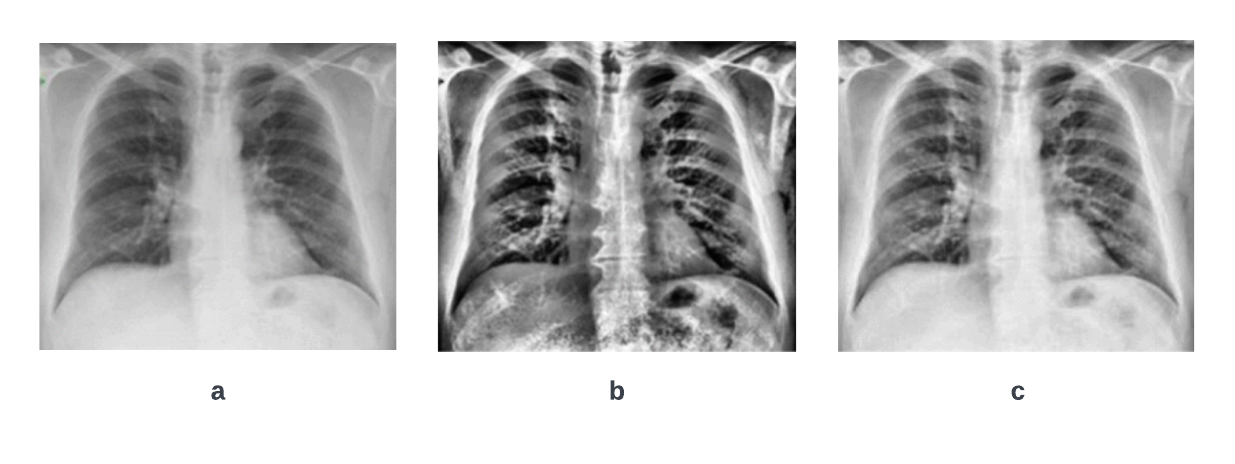
\includegraphics[width=1\textwidth]{obrazky/CLAHEvsAHE.png}
	\caption{Aplikace různých typů histogramové ekvalizace. (a) původní obraz, (b) AHE, (c) CLAHE \cite{9563980}}
	\label{CLAHEvsAHE}
\end{figure}


\subsection{Binarizace - adaptivní prahování}
\label{adaptivetresh_chapter}
Binarizace je převod šedotónového obrazu na jeho černobílou reprezentaci. Toho se dá dosáhnout pomocí \textbf{prahování}. Prahování je metoda, v které intenzita výsledného pixelu závisí na intenzitě vstupního pixelu a hodnotě prahu. Konkrétně se tak děje porovnáváním intenzity pixelu s hodnotou prahu a v případě, že je intenzita větší nežli je hodnota prahu se pixel obarví na bílo (intenzita s hodnotou 255), v opačném případě se pixel obarví na černo (intenzita s hodnotou 0). Hlavním problémem klasického prahování na základě jedné hodnoty prahu je binarizace obrazu s proměnlivým osvětlením. V tomto případě se totiž díky osvětlení intenzity pixelů liší v různých částech obrazu a tudíž je jedna hodnota prahu nedostačující.

Z tohoto důvodu existuje \textbf{adaptivní prahování}. Tato metoda rozděluje obraz na bloky, v kterých se pomocí statistických ukazatelů obrazu určí hodnota prahu pro daný blok a následně se v něm provede binarizace. Určení této hodnoty se může dělat několika způsoby. Mezi nejpoužívanější patří určení prahu na základě střední hodnoty\footnote{Střední hodnota vznikne sečtením hodnot všech pixelů v požadované oblasti. Následně se tato hodnota podělí počtem hodnot a tím vznikne střední hodnota neboli průměr.} pixelů v bloku, nebo výpočet hodnoty prahu na základě intenzit pixelů v bloku vynásobeným Gaussovým jádrem. Na následujícím obrázku bude uvedena ukázka rozdílu mezi klasickým prahováním a adaptivním prahováním s různými jádry \ref{prahovani}.

\newpage
\begin{figure}[h]
	\centering
	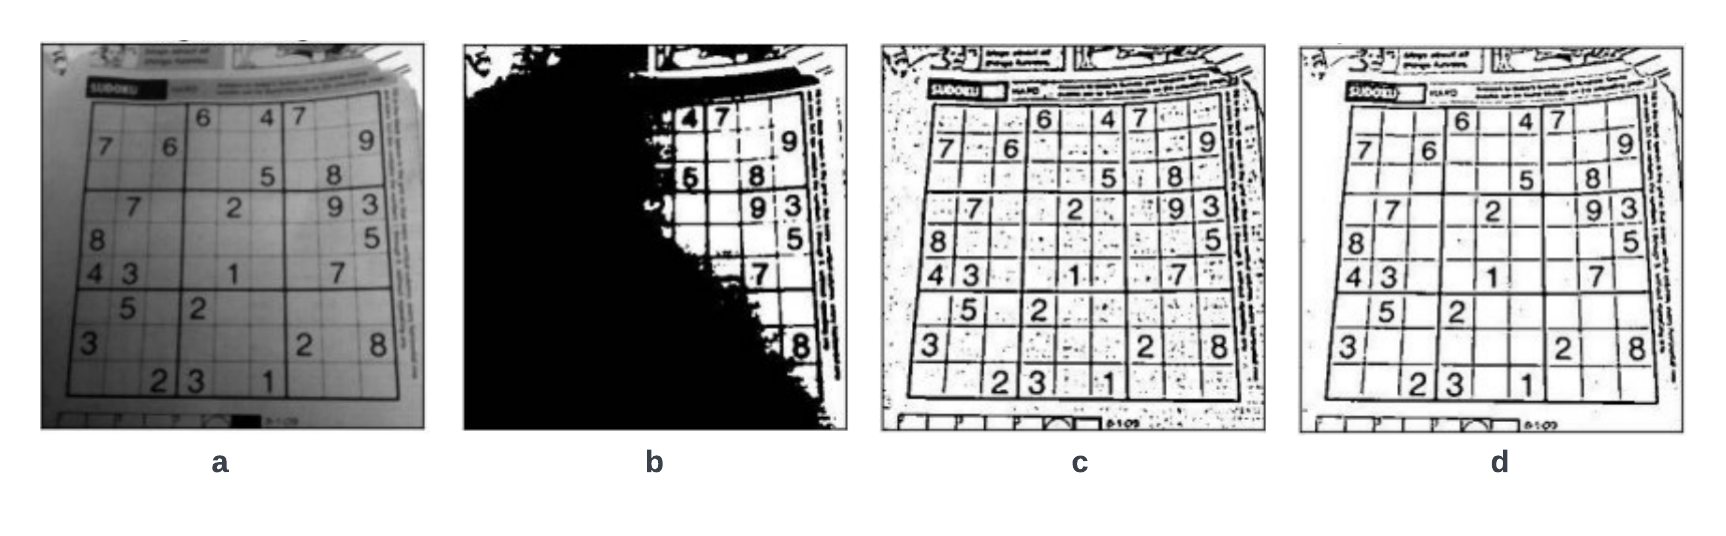
\includegraphics[width=1\textwidth]{obrazky/prahovani.png}
	\caption{Binarizace pomocí prahování. (a) původní obraz, (b) klasické prahování (hodnota práhu je 127), (c) adaptivní prahování na základě střední hodnoty, (d) adaptivní prahování na základě Gaussova jádra \cite{opencv_doc}}
	\label{prahovani}
\end{figure}


\subsection{Kontury - momenty, hiearichie, huul}
\label{kontury_chapter}
%https://docs.opencv.org/3.4/d3/d05/tutorial_py_table_of_contents_contours.html
\textbf{Kontury} jsou důležitým pojmem v oblasti počítačového vidění, konkrétně jsou užitečné pro analýzu tvaru nebo detekci a rozpoznání objektů v obraze. Konturu lze definovat jako křivku, která je tvořena body podél hranice se stejnou intenzitou. Tyto kontury lze vyhledávat jak v černobílém tak v šedotónovém obraze, ovšem jelikož intenzity hran v šedotónovém obraze nebývají stejné, může v něm být vyhledávání kontur nevhodné. Co se týče černobílého obrazu, je nutné aby byly hledané objekty reprezentovány bílou barvou, jelikož to aktuální implementace knihovny openCV vyžaduje pro správné nalezení kontur. Hlavní výhodou reprezentace objektů pomocí kontur je množina operací a vlastností, které nad nimi openCV poskytuje. Dále se text bude věnovat vysvětlením několika základních pojmů a operací, které jsou s konturami spjaty, jelikož se s nimi bude v práci dál pracovat.   


\textbf{Reprezentace kontury} může být provedena buď pomocí vrcholů, které konturu tvoří, nebo pomocí úplné kopie hran. Kopie hran zabírá příliš místa a není pro tuto práci příliš důležitá, tudíž je výhodnější použít bodovou reprezentaci. Na následujícím obrázku bude zobrazen rozdíl mezi těmito dvěma reprezentacemi \ref{body_kontury}.

\begin{figure}[h]
	\centering
	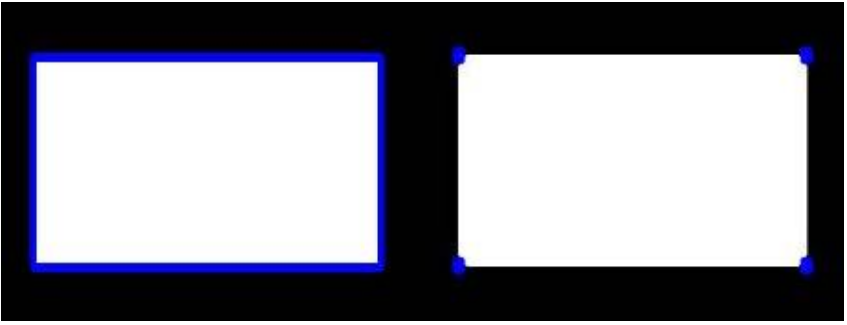
\includegraphics[width=0.8\textwidth]{obrazky/body_kontury.png}
	\caption{Způsoby aproximace kontury, nalevo se nachází kopie hran a napravo vrcholová reprezentace \cite{opencv_doc}}
	\label{body_kontury}
\end{figure}

\newpage
Dále jsou důležité struktury, v nichž lze reprezentovat \textbf{uspořádání kontur}. Pro tuto práci bude nejdůležitější reprezentace listová a stromová. Listová reprezentace je způsob, který nijak nereflektuje uspořádání kontur a pouze obsahuje všechny nalezené kontury. Stromová reprezentace na rozdíl od listové umožňuje zjistit, které kontury jsou obsaženy v jiných.

\textbf{Momenty} jsou matematické funkce, kterými se popisují různé vlastnosti dané kontury. Mezi vlastnosti důležité pro tuto práci patří plocha a střed kontury. Ukázka rovnice popisující konturu se nachází níže \ref{moment_base}.
Výpočet \textbf{plochy kontury} je poté už pouze suma světlých pixelů přes ohraničující okno neboli se jedná o hodnotu $M_{00}$ dosazenou do vzorečku \ref{moment_base}. 
Pro výpočet souřadnic \textbf{středu kontury} se poté používá vzorec \ref{centroid_eq}.

\begin{equation}
    M_{ab} =  \sum_{x} \sum_{y} x^a y^b I(x,y)
    \label{moment_base}
\end{equation}


\begin{equation}
    \{x,y\} =  \{\frac{M_{10}}{M_{00}}, \frac{M_{01}}{M_{00}}\}
    \label{centroid_eq}
\end{equation}

Dalším pojmem je tzv. \textbf{Huulova aproximace}, která dokáže určit konvexní konturu na základě té původní. Ukázka vizualizace Huulovy aproximace je na následujícím obrázku \ref{huul}. Původní kontura je zde reprezentována obrysem ruky a její Huulova aproximace je znázorněna červenou. 

\begin{figure}[h]
	\centering
	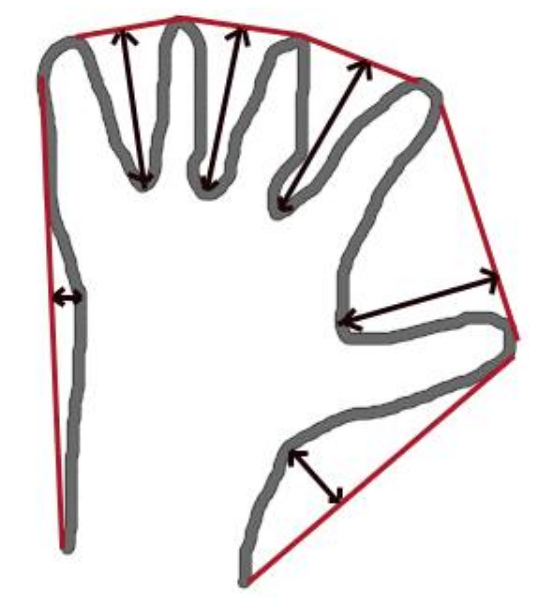
\includegraphics[width=0.4\textwidth]{obrazky/huul.png}
	\caption{Huulova aproximace původní kontury \cite{opencv_doc}}
	\label{huul}
\end{figure}

Konvexní aproximaci lze využít pro určení úplnosti. \textbf{Úplnost} se vypočítá jako poměr ploch původní kontury vůči aproximované konvexní Huulově kontuře. Díky tomu lze v této práci určit, jak moc je kontura poškozená, respektive jak dobře byla kontura určena pro původní polygon. 



\subsection{Morfologické operace - otevření}
\label{morpho_chapter}
Morfologické operace jsou matematické transformace, které pomocí aplikace strukturního elementu upravují obraz. Strukturní element je malý obrazec, který je obvykle definován jako malá matice nebo jádro. Strukturní element může nabývat různých tvarů jako například čtverec, obdélník a kříž viz \ref{element}. Jeho velikost a tvar pak určuje, jaký druh transformace bude proveden na vstupní obraz. Při aplikaci se strukturní element posouvá přes vstupní obraz a určuje, jak se změní hodnoty pixelů výstupního obrazu.


\begin{figure}[h]
	\centering
	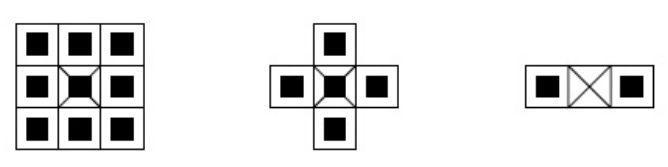
\includegraphics[width=0.8\textwidth]{obrazky/strukturalni_element.png}
	\caption{Základní typy strukturních elementů \cite{morfologie}}
	\label{element}
\end{figure}

Morfologické operace pracují s binárním nebo šedotónovým obrazem a používají se například pro detekci hran, segmentaci obrazu, odstranění šumu (detailů) a ztenčování nebo rozšiřování objektů. V této práci se budou morfologické operace používat na binární obraz. Mezi základní morfologické operace patří eroze, dilatace, otevření a uzavření. Operace typu uzavření zde ovšem nebude vysvětlena, jelikož to není potřeba vzhledem k povaze práce. 

\textbf{Dilatace} je druh operace, který se používá k vyplnění malých děr, rozšiřování objektů a tvoří základ pro složitější morfologické operace jako otevření a uzavření. Na následujícím obrázku bude ukázka aplikace dilatace \ref{aplikace_dilatace}.

\begin{figure}[h]
	\centering
	
\includegraphics[width=0.8\textwidth]{obrazky/dilatace.png}
	\caption{Aplikace dilatace na vstupní obraz se strukturálním elementem o rozměrech 3x3 \cite{morfologie}}
	\label{aplikace_dilatace}
\end{figure}

\textbf{Eroze} je operace, která je duální vůči dilataci. Používá se pro odstranění a ztenčení objektů v obraze nebo umožňuje získat obrys objektu. Stejně jako dilatace tvoří základ pro složitější morfologické operace. Na následujícím obrázku bude uvedena ukázka aplikace eroze \ref{aplikace_eroze}.


\newpage
\begin{figure}[h]
	\centering
	
\includegraphics[width=0.8\textwidth]{obrazky/eroze.png}
	\caption{Aplikace eroze na vstupní obraz se strukturálním elementem o rozměrech 3x3 \cite{morfologie}}
	\label{aplikace_eroze}
\end{figure}

\textbf{Morfologické otevření} je operace, která využívá kombinace eroze a dilatace. Díky její aplikaci je možné získat obraz, kde budou odděleny úzce spojené objekty a odstraněny malé detaily \cite{morphology_opening}. Tato operace byla vytvořena kvůli tomu, že eroze nejen odstraňuje malé detaily v obraze, ale také ztenčuje objekty v něm. Z tohoto důvodu se na obrázek aplikuje dilatace, která obnovuje původní šířku objektů a současně ponechává odstraněné detaily. Otevření je tedy ve výsledku eroze následovaná dilatací. Na následujícím obrázku bude ukázka aplikace morfologického otevření \ref{aplikace_otevreni}.

\begin{figure}[h]
	\centering
	
\includegraphics[width=0.8\textwidth]{obrazky/otevreni_ukazka.png}
	\caption{Aplikace morfologického otevření na vstupní obraz se strukturálním elementem o rozměrech 3x3 \cite{morfologie}}
	\label{aplikace_otevreni}
\end{figure}

\section{Návrh systému}

Systém bude fungovat jako konzolová aplikace, kde uživatel zadá cestu ke vstupní fotografii a případně cestu ke složce s šablonami, s kterými chce fotografii porovnat. V případě, že uživatel nebude chtít fotografii porovnávat, vypíše se mu na standardní výstup textová reprezentace vstupní fotografie (šablona markantů). Celkově se systém bude skládat ze čtyř částí. Na začátku je potřeba z fotografie získat oblast zájmu. Ta se získá pomocí rotace a změny velikosti, díky kterým bude výsledná oblast zájmu ve stejném formátu pro další rozpoznávání. Následně je potřeba oblast zájmu předzpracovat. Toho se docílí pomocí dolnopropustního filtru zachovávající hrany. Následně se na obrázek aplikuje kontrastní vylepšení, které následujícím algoritmům pomůže se správným rozpoznáním polygonů. Před samotným určením těchto polygonů je třeba obraz binarizovat a následně v něm opravit možné chyby. Toho se docílí pomocí opravy kontur. Následně se na obraz použijí morfologické operace, které způsobí oddělení kontur v místech, kde pří binarizaci vznikl malý spoj. Následně se redukuje počet kontur. Toho se dosáhne pomocí řady filtrů, které byly navrženy tak aby z binarizovaného obrazu odstranily porušené kontury, které by mohly způsobit nepřesné určení markantů. Poté se nalezené markanty převedou do textové reprezentace (šablony) a vypíší na standartní výstup a nebo se provede porovnávání s ostatními šablonami. V případě, že si uživatel zvolil možnost s porovnáváním se postupně prochází složka s šablonami a postupně se porovnávají. Nakonec se na základě procentuální podobnosti šablon určí, který obraz nejlépe odpovídá tomu vstupnímu. Na následujícím obrázku je ukázka navrženého systému \ref{navrh_systemu}.


\begin{figure}[h]
	\centering
	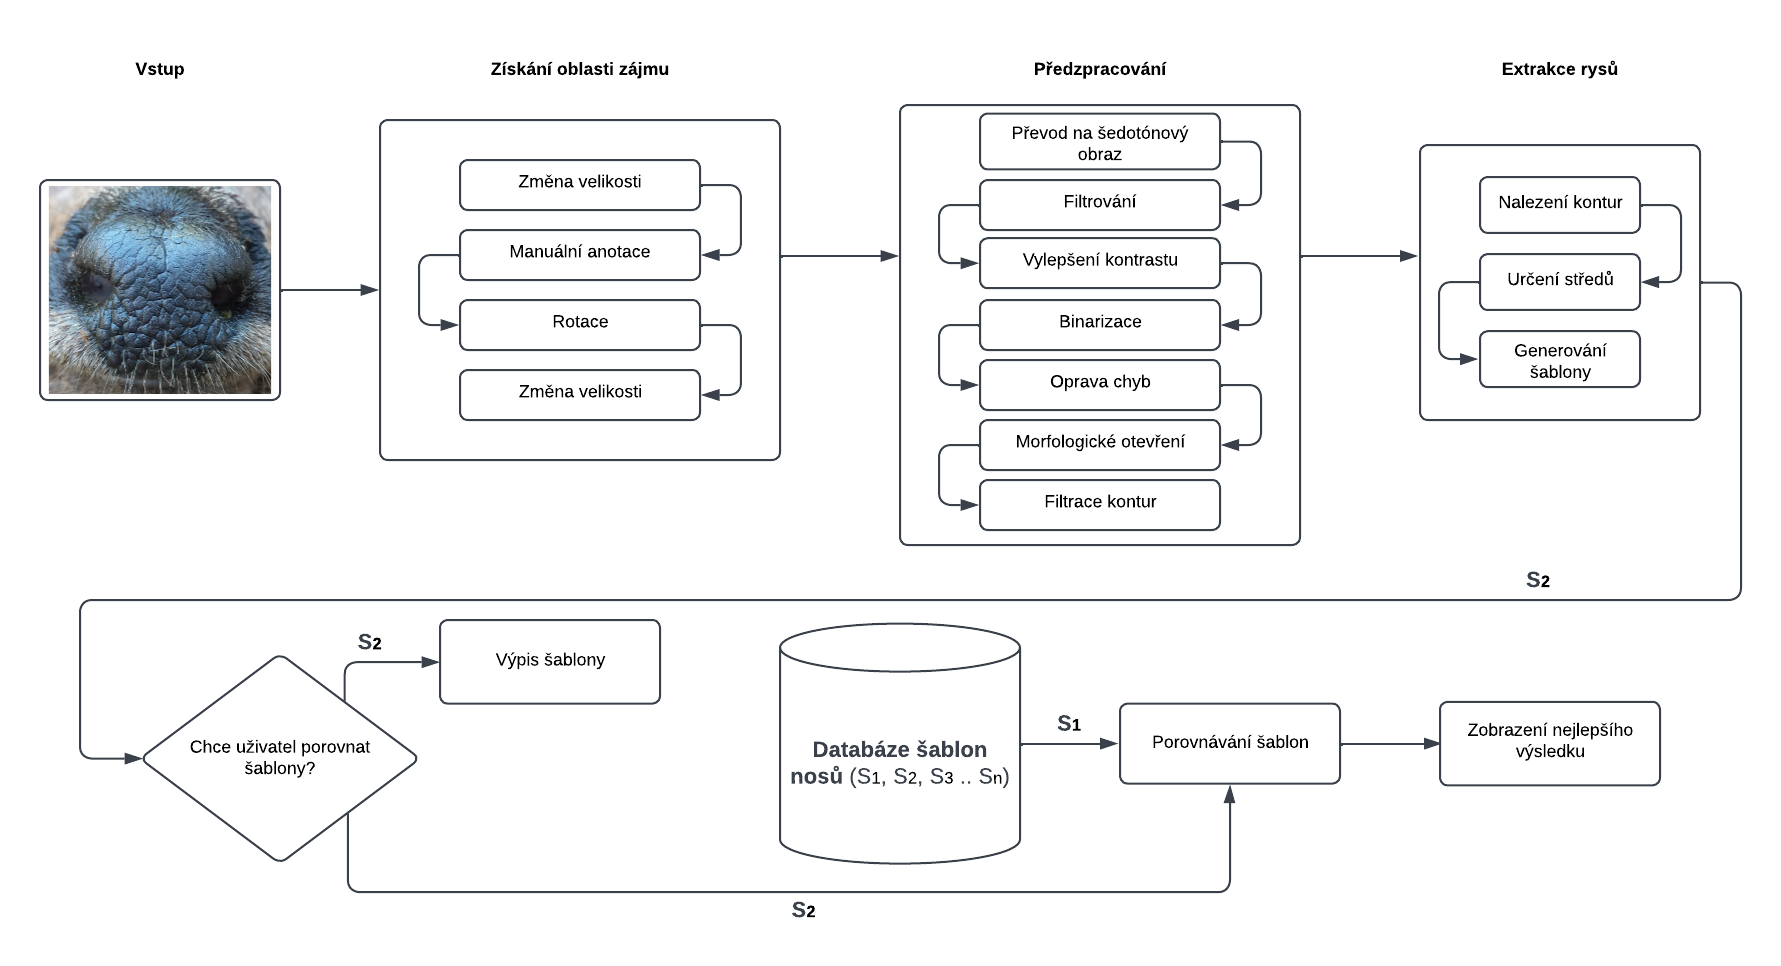
\includegraphics[width=1\textwidth]{obrazky/navrzeny_system.png}
	\caption{Navržený systém pro rozpoznávání zvěře na základě fotografie nosu}
	\label{navrh_systemu}
\end{figure}


\subsection{Získání fotografií nosů}
Vstupem do systému jsou fotografie nosů zvěře. Ty jsou získány z experimentální databáze nosů zvěře, která byla vytvořena pro tento účel. Fotky v této databázi byly pořízeny v terénu dobrovolníky po zabití jedince zvěře. Pro každého takového jedince byla pořízena sada fotek. Způsob pořizování fotografií je prozatím neustálený z hlediska směru, osvětlení (používání blesku) a okolních vlivů. Příkladem těchto vlivů může být například vlhkost na čumáku, která při fotografii s bleskem způsobí, že je fotografie téměř nepoužitelná pro rozpoznávání. Dalším takovým vlivem mohou být nečistoty na čumáku jako třeba malé listy případně jiné objekty, které mohou na čumáku zůstat po odstřelu pří nedostatečném očištění. Mezi další nejčastější problémy patří nedostatečné zaostření na oblast rhinaria a špatný úhel při pořizování fotografie. Prozatím je v této databázi přes 2000 fotografií a pro účel této práce bylo vybráno 171 fotek, které splňovali autorem určená kritéria. Hlavním kritériem při výběru fotek byla hlavně kvalitně zaostřená a dobře viditelná oblast rhinaria. Jelikož bylo v zájmu vyzkoušet tento přístup na různé typy fotek, byla tato databáze doplněna o fotky, které nebyly úplně ideální a obsahovaly různé problémy, které byly popsány dříve. Nejčastěji byly fotografie byly pořizovány mobilním telefonem, aby nebylo nutné používat žádné zvláštní zařízení. Z důvodu možného pohoršení čtenáře budou na následujícím obrázku ukázány pouze ořezané fotky možných vstupních fotografií bez zbytku usmrcené zvěře \ref{ukazka_fotek}.

\begin{figure}[h]
	\centering
	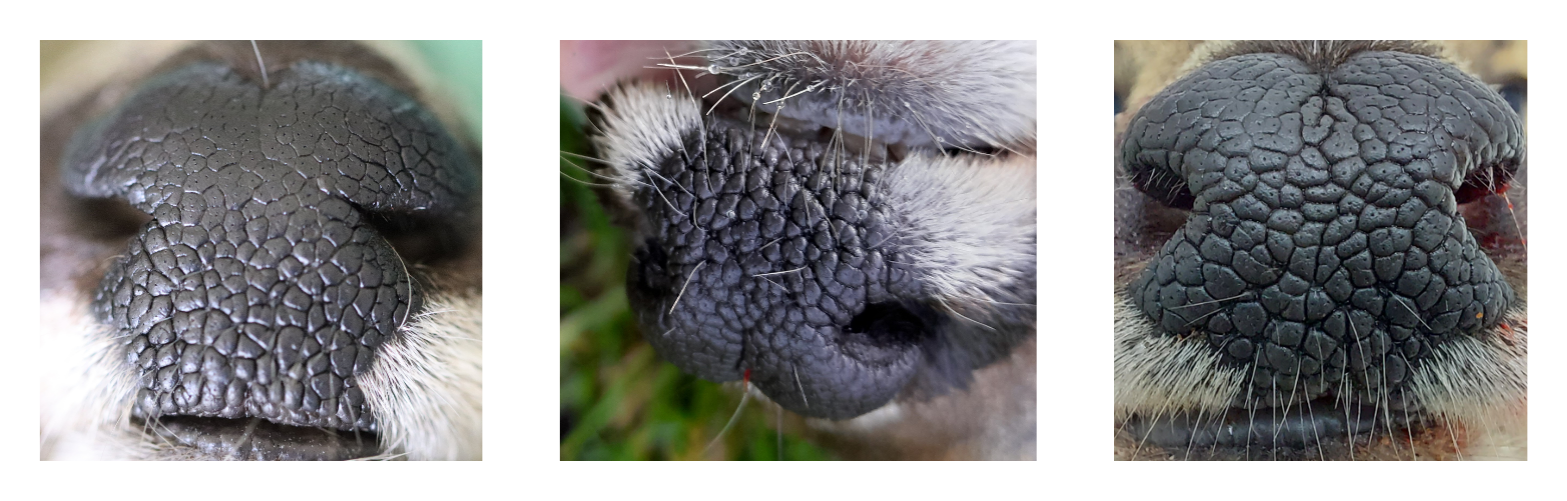
\includegraphics[width=1\textwidth]{obrazky/fotky_ukazka.png}
	\caption{Ořezané fotografie nosů zvěře}
	\label{ukazka_fotek}
\end{figure}

\subsection{Získání oblasti zájmu}
Jelikož jsou fotografie focené z větší vzdálenosti, obsahují kromě oblasti rhinaria i různé nevyžádané prvky. Navíc mají fotografie i různé velikosti, což je pro další postup nevhodné. Pro tento účel je potřeba získat tzv. oblast zájmu. \textbf{Oblast zájmu} je část původní fotografie, která obsahuje pouze rhinarium a je již rotačně a velikostně převedena do stavu, který je vhodný pro další postup. Zároveň oblast zájmu představuje i souřadnicový systém, ve kterém se budou nacházet markanty.

Na základě pozorování bylo zjištěno, že vyhovujícími body pro ohraničení této oblasti budou nosní dírky. První myšlenkou pro automatické zajištění těchto bodů byla jejich barva. Teoreticky by nosní dírky měly být nejtmavší. To se ovšem ukázalo jako nepravdivé, jelikož nestejný způsob osvětlení fotografií způsoboval, že nosní dírky nebyly nejtmavší, tudíž bylo od tohoto způsobu upuštěno. 

Další variantou by bylo využít strojového/hlubokého učení, aby se tyto body ohraničující nosní dírky určily automaticky. Z důvodu nedostatku dat pro natrénování je tato možnost ovšem velice omezená a nemusela by správně fungovat.

Z těchto důvodů se nakonec zvolila uživatelsky nepohodlná ale zato spolehlivá metoda založená na manuální anotaci nosních dírek. V potaz při anotaci byl brán i horní ret, ovšem po zvolení způsobu ořezání oblasti zájmu se od toho opustilo, jelikož se pozice rtu nijak nevyužívalo. Ukázka návrhu získání oblasti zájmu na základě anotace \ref{ziskaniROI}.

\newpage
\begin{figure}[h]
	\centering
	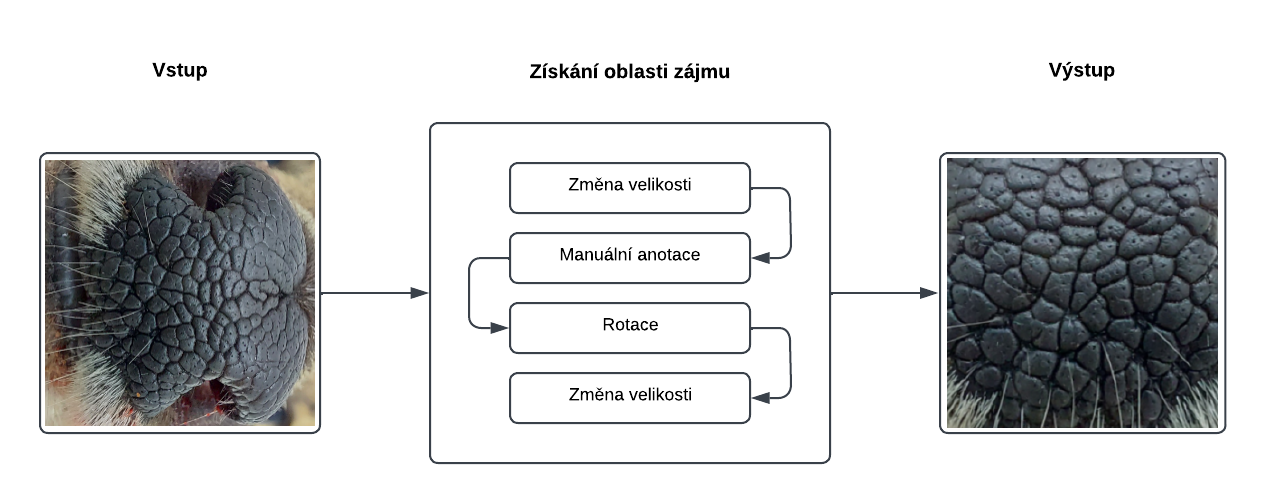
\includegraphics[width=1\textwidth]{obrazky/ziskani_oblasti.png}
	\caption{Návrh získání oblasti zájmu}
	\label{ziskaniROI}
\end{figure}

Ještě před samotnou anotací je potřeba vstupní fotografii zmenšit, aby nebyla příliš velká pro zobrazení uživateli. To se udělá pomocí změny velikosti obrazu v takovém poměru, aby výsledná fotografie měla šířku 600 pixelů a výšku určenou na základě poměru původní šířky vůči 600 pixelům. Díky tomu si vstupní fotografii zachová poměr stran a nebude nijak deformovaná.

\subsubsection{Manuální anotace}

Jedna nosní dírka se označí celkem třemi body, jelikož je to nejmenší počet bodů pro označení nějaké oblasti. Pozice prvního bodu je v případě levé nosní dírky její nejpravější bod. V případě pravé nosní dírky je to naopak nejlevější bod. Na základě těchto bodů bude možné určit, kde začíná rhinarium a kde končí nosní dírka. Díky tomu jsou tyto body vhodné pro určení šířky výsledné oblasti zájmu. Tyto dva body se budou dále nazývat jako \textbf{delty}, jelikož se pomocí nich bude určovat pozice vyextrahovaných rysů, což má jistou podobnost s deltami u otisků prstů. Navíc je možné tyto body nejjednoznačněji určit a tudíž se jeví jako nejvhodnější pro následný postup. Další dva body pro anotaci nosní dírky jsou její nejvrchnější bod a nejspodnější bod. Při anotování je důležité pořadí, v kterém jsou body označeny. Prvně se body označuje levá dírka a až poté ta pravá. Bez zachování pořadí by nebylo možné určit, která nosní dírka je pravá a která levá, což by způsobilo špatnou rotaci obrazu. Na následujícím obrázku bude ukázáno, jak se fotografie anotuje \ref{anotace}.

\newpage
\begin{figure}[h]
	\centering
	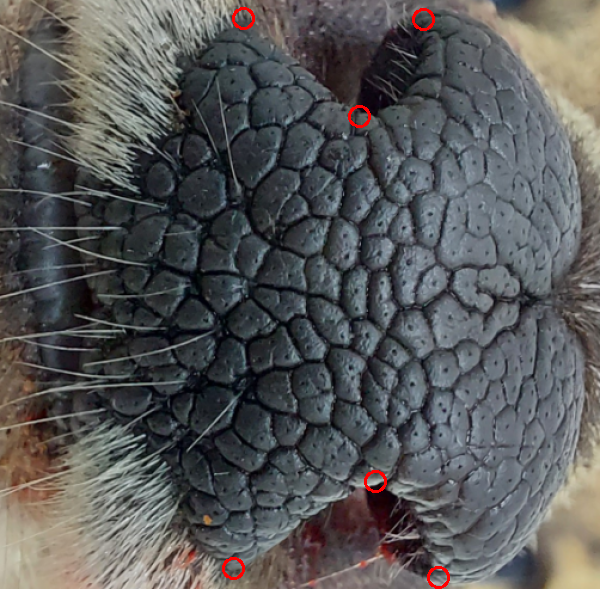
\includegraphics[width=0.45\textwidth]{obrazky/1_points.png}
	\caption{Anotace nosních dírek}
	\label{anotace}
\end{figure}

\subsubsection{Rotace}

Původně bylo v plánu pomocí anotovaných bodů udělat okolo obou nosních dírek vepsané nebo opsané kružnice. Za pomocí středů těchto kružnic by se obrázek otočil, aby byl rotačně normalizován.


Dalším důvodem těchto bodů byla kromě vyříznutí oblasti zájmu transformace perspektivy, která by zajistila, že se fotografie pořízeny pod různými úhly transformují do stavu, který by odpovídal frontální fotografii. Od toho se nakonec upustilo, jelikož nosní dírky občas nebyly vidět celé a tudíž bylo těžké anotovat dírky na správných místech. Například v případě že je fotografie focena více ze strany, je velice obtížné anotovat nosní dírku vrchním a spodním bodem, jelikož nejde pořádně poznat, kde dírka končí \ref{anotace_problem}.

\begin{figure}[h]
	\centering
	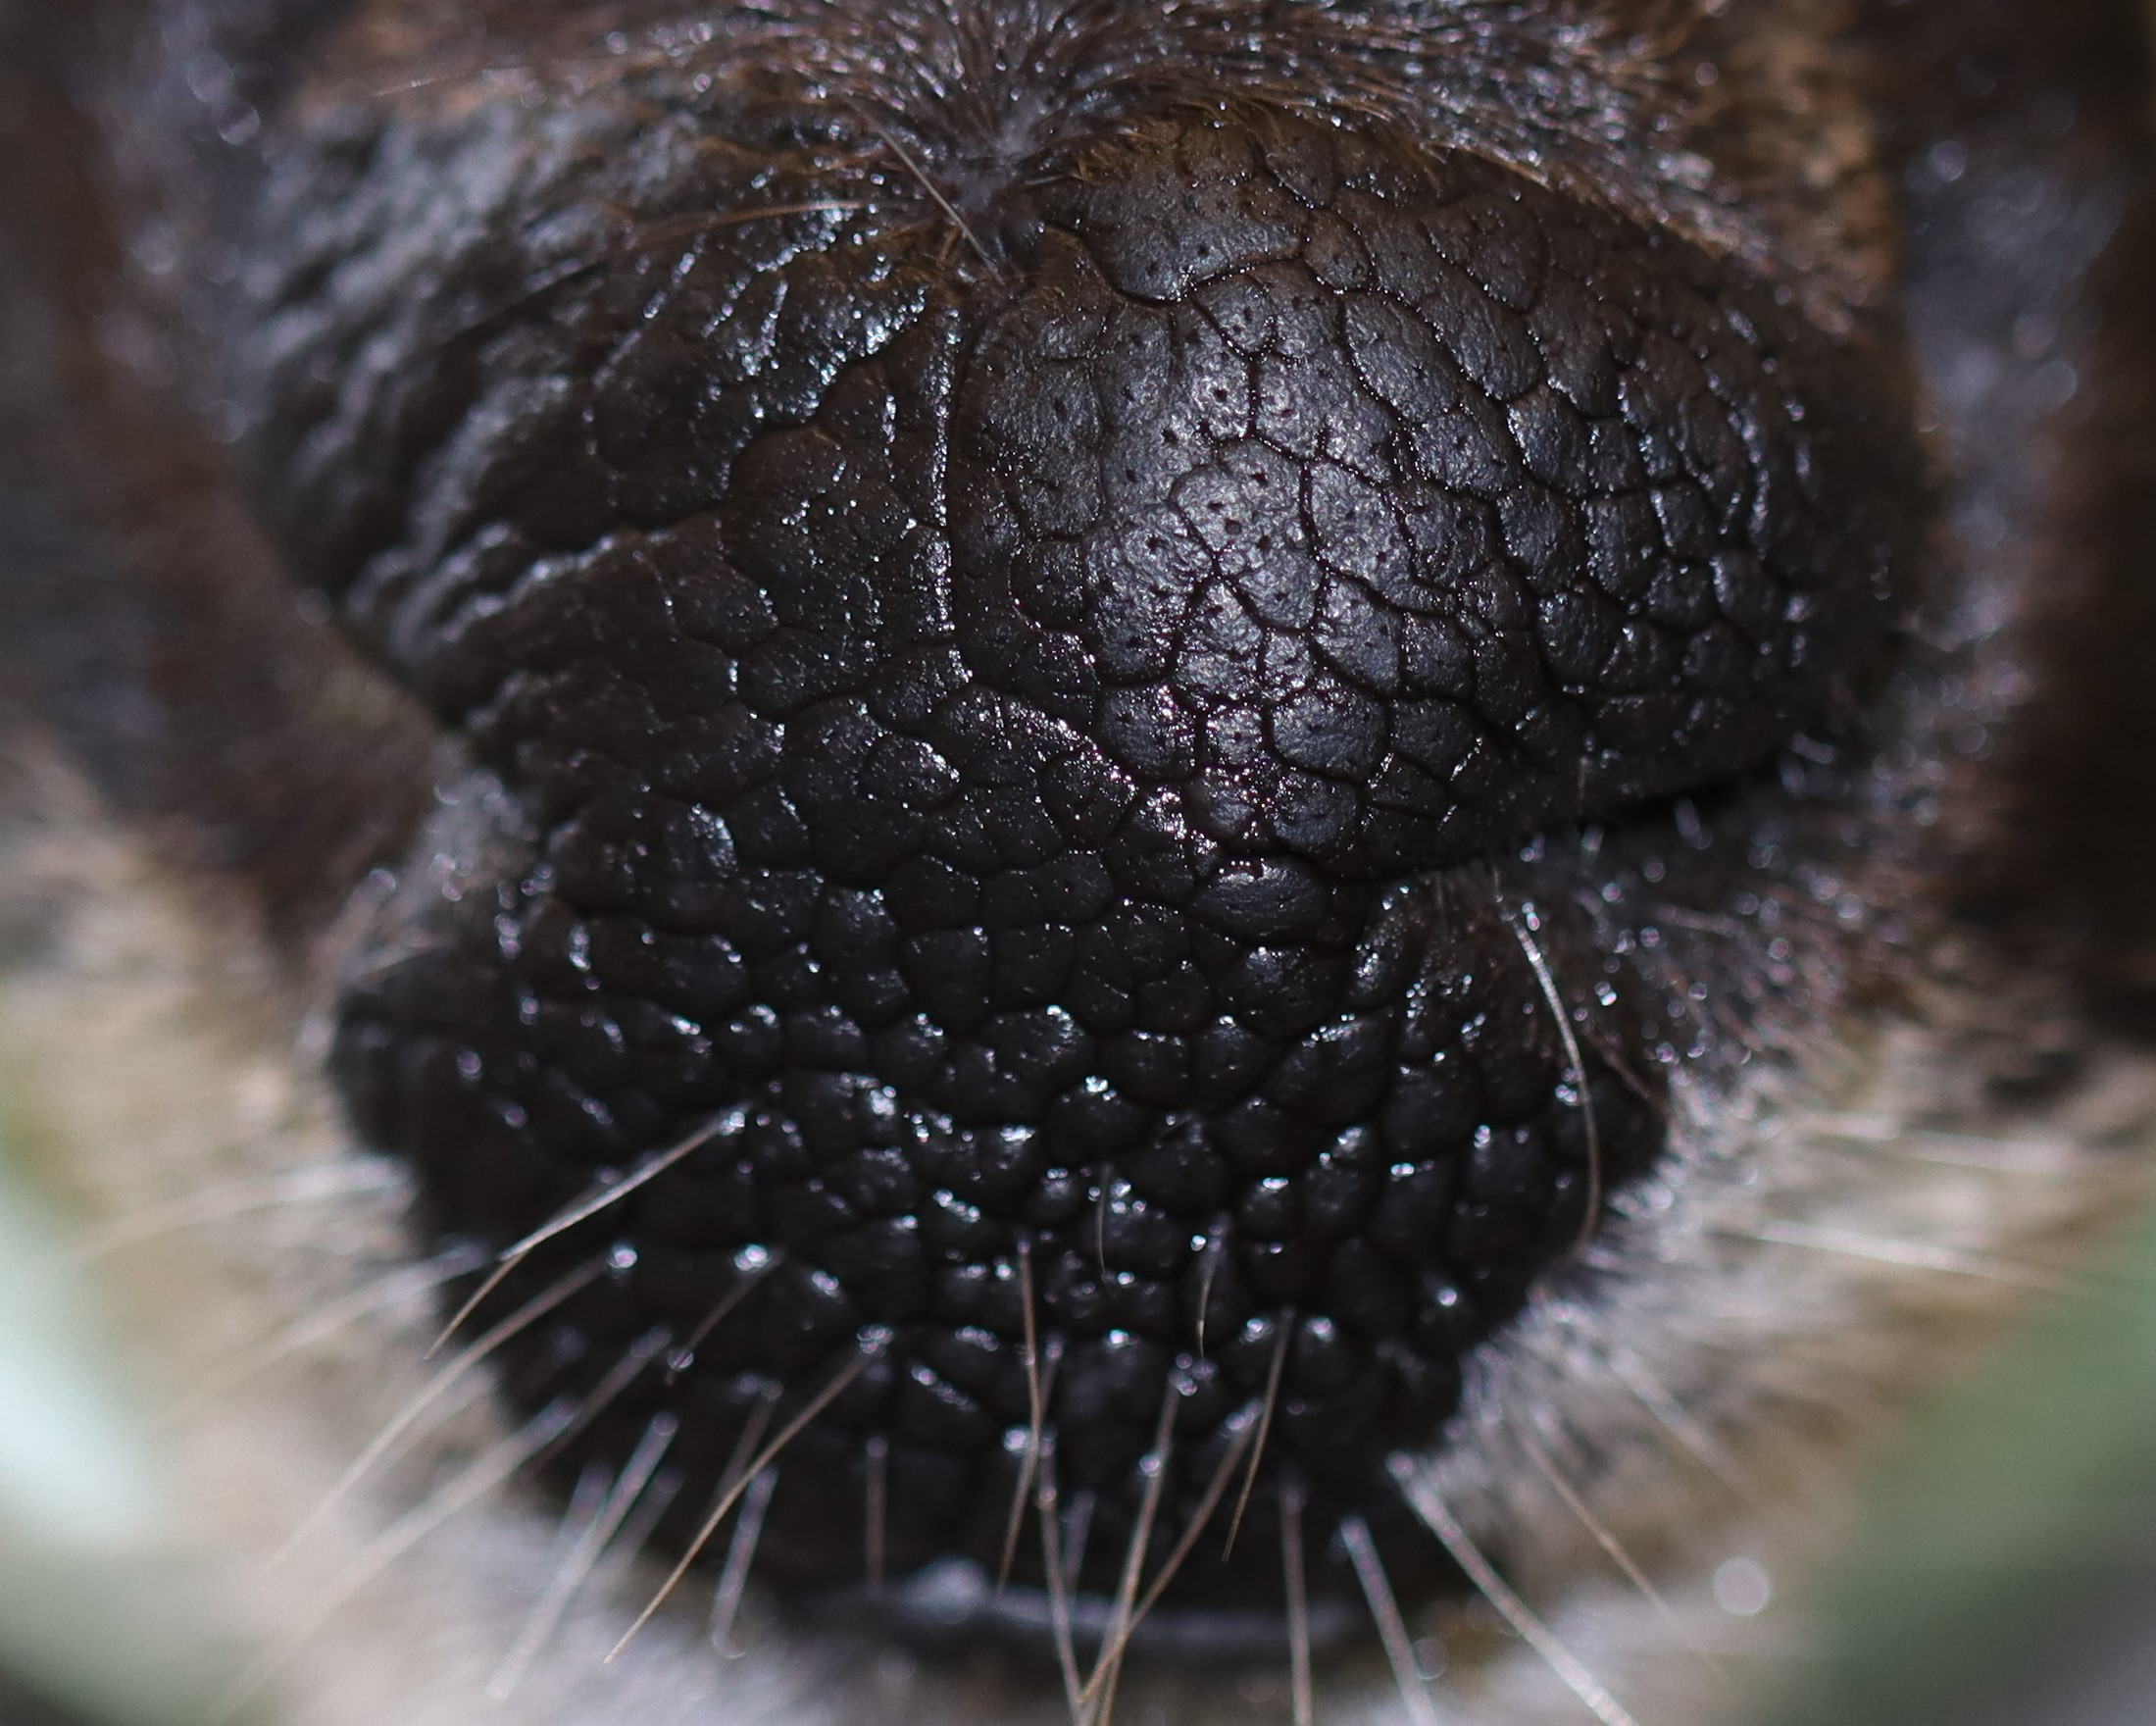
\includegraphics[width=0.45\textwidth]{obrazky/dirka_problem.JPG}
	\caption{Problémová fotografie pro anotaci}
	\label{anotace_problem}
\end{figure} 

Z těchto důvodů se od kružnic opustilo. Rotace se dělá na základě pozic samotných delt. Díky tomu je oblast zájmu orotovaná na základě bodů, které byly potřebné pro její vyříznutí. Výsledek orotované fotografie lze vidět na následujícím obrázku \ref{rotated}.


\begin{figure}[h]
	\centering
	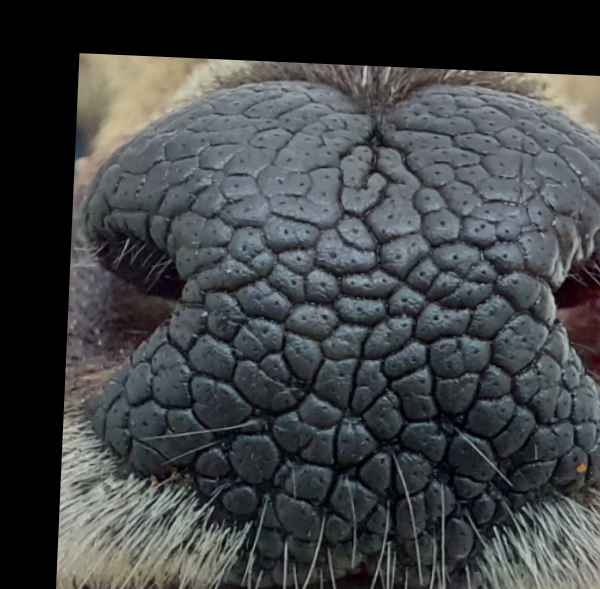
\includegraphics[width=0.45\textwidth]{obrazky/2_rotated.png}
	\caption{Orotovaná fotografie na základě delt}
	\label{rotated}
\end{figure} 

\subsubsection{Získání oblasti zájmu}

Cílem této části bylo získat z fotografie co největší část rhinaria a zároveň zajistit aby výsledná oblast neobsahovala ostatní části fotografie. Z těchto důvodů bylo vyzkoušeno několik útvarů s různým posunutím. Co se týče velikosti oblasti zájmu bylo na základě experimentování dospěno k závěru, že nejlepším útvarem je čtverec, který měl délku strany o vzdálenosti mezi deltami. Dále byl tento čtverec posunut o čtvrtinu délky strany dolů, jelikož pokud byly delty na středu, výsledná oblast neobsahovala pouze rhinarium ale i ostatní části fotografie. Výsledkem této části je oblast zájmu, která bude správně orotovaná a bude mít pevnou velikost 300x300 pixelů. Ukázka výsledné oblasti zájmu je vidět napravo na obrázku \ref{ziskaniROI}.


\subsection{Předzpracování}

Předzpracování fotografie je proces, který pracuje se získanou oblasti zájmu. Úkolem \\ předzpracování je převedení oblasti do takové podoby, aby byla vhodná pro extrakci rysů. Prvním krokem předzpracování je převod obrazu na jeho šedotónovou variantu. Následně je vhodné obraz vyfiltrovat, aby se v něm redukoval šum. Po filtrování následuje vylepšení kontrastu rýh a polygonů. Vylepšený obraz poté poslouží jako vstup pro binarizaci. Tím vznikne dvouúrovňová reprezentace obrazu. Následně se v obrazu najdou kontury, u kterých dojde k jejich vylepšení. Poté se na obraz s konturami aplikují morfologické operace, aby se oddělily možné spojitosti v místech, kde by být neměly. Na obraz se nakonec aplikuje řada filtrů, které odstraní špatně rozpoznané kontury. Ukázka návrhu předzpracování obrazu se nachází na \ref{predzpracovani_navrh}.


\newpage
\begin{figure}[h]
	\centering
	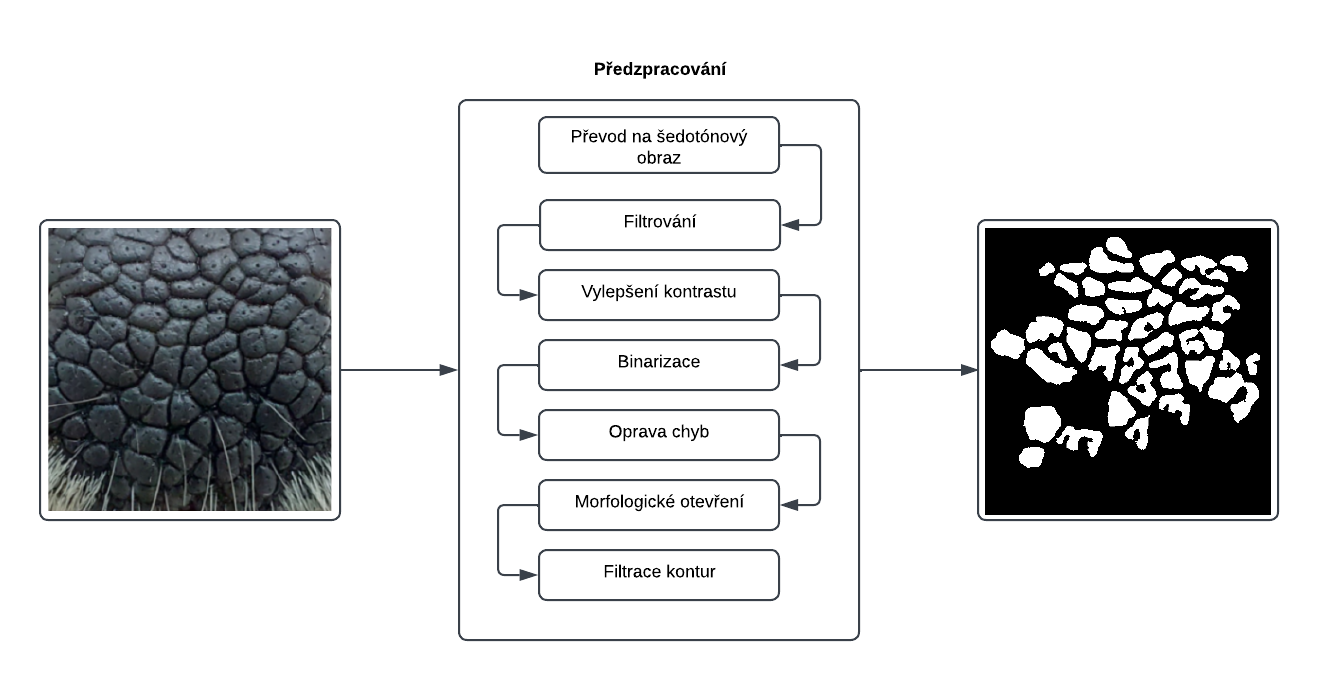
\includegraphics[width=1\textwidth]{obrazky/predzpracovaniv2.png}
	\caption{Návrh předzpracování oblasti zájmu}
	\label{predzpracovani_navrh}
\end{figure} 

\subsubsection{Převod na šedotónový obraz}

Tento krok se provádí za účelem snížení výpočetní náročnosti aplikovaných algoritmů. Operace pracuje po pixelech a každý pixel složený ze tří komponent (modrá, zelená, červená) převede na jednu hodnotu intenzity dle vah jednotlivých komponent. Ukázka šedotónového obrazu se nachází na obrázku \ref{filtr} společně s vyfiltrovaným obrazem.


V případě potřeby by bylo v tomto kroku možné určit, zda je obrázek vhodný pro další zpracování. Toho by se dalo dosáhnout pomocí analýzy histogramu daného obrazu. Na základě počtu světlých pixelů by bylo možné určit, jestli se v obraze nenachází příliš odlesku, což téměř znemožní další zpracování \cite{psi}.

\subsubsection{Filtrace obrazu}

Pro filtrování je navrženo několik dolnopropustních filtrů jako Gaussův filtr, mediánový filtr, průměrový filtr a bilaterální filtr. Úkolem tohoto filtru bude kromě redukce šumu také co nejlepší zachování původních rýh a polygonů. Na základě těchto kritérií a řadě testování, byl pro tento krok zvolen bilaterální filtr \ref{bilateral_chapter}. Ten je sice výpočetně pomalejší, ovšem ve srovnání s ostatními navrženými filtry vykazoval nejlepší výsledky. Na následujícím obrázku je uvedena ukázka aplikovaného filtru na šedotónový obraz \ref{filtr}.

\newpage
\begin{figure}[h]
	\centering
	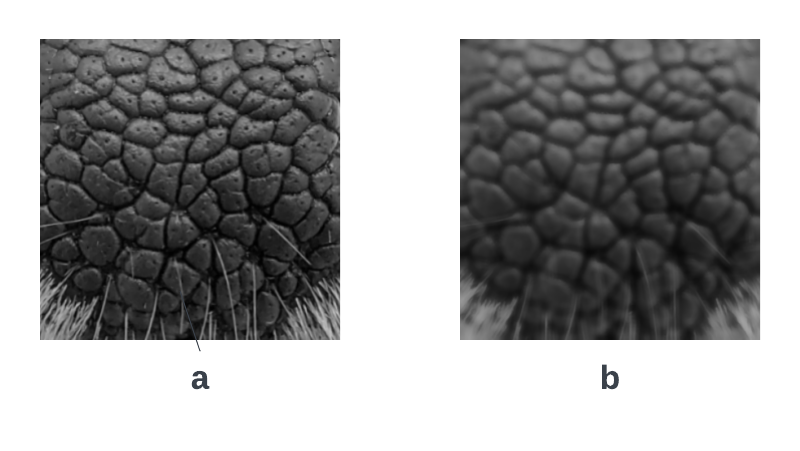
\includegraphics[width=0.6\textwidth]{obrazky/filtr.png}
	\caption{Obrázek před a po filtraci. (a) šedotónový obraz, (b) obraz po aplikaci bilaterálního filtru}
	\label{filtr}
\end{figure} 

\subsubsection{Vylepšení kontrastu}

Po filtrování se v obrazu vylepší kontrast rýh a polygonů. Toho se dá dosáhnout pomocí histogramové ekvalizace \ref{ekvalizace_chapter}, která způsobí, že intenzity pixelů se rozprostřou po celém spektru. Algoritmus zvolený pro tento krok se nazývá CLAHE a jedná se o vylepšenou variantu klasické histogramové ekvalizace. Tento přístup byl zvolen na základě práce o rozpoznávání psů na základě nosu \cite{psi},~~jelikož nosy srnek a jelenů mají barevně nos podobný tomu psímu. Na následujícím obrázku se nachází ukázka před a po vylepšení kontrastu včetně porovnání s klasickou histogramovou ekvalizací \ref{clahe}.


\begin{figure}[h]
	\centering
	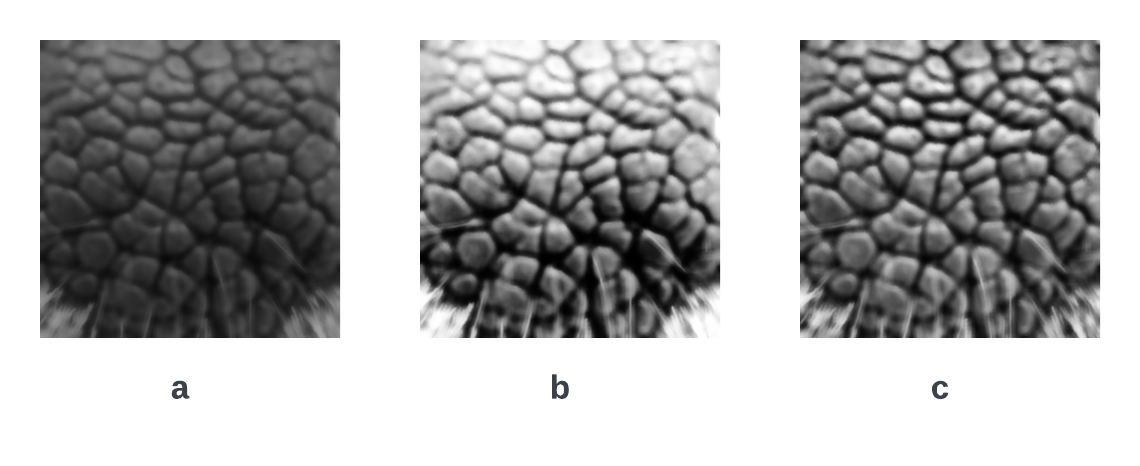
\includegraphics[width=0.9\textwidth]{obrazky/clahe2.png}
	\caption{Aplikace histogramové ekvalizace na obraz. (a) původní obraz, (b) histogramová ekvalizace, (c) CLAHE}
	\label{clahe}
\end{figure} 


\subsubsection{Binarizace}

Po kontrastním vylepšení bude následovat binarizace. Ta převede šedotónový obraz do černobíle reprezentace. K tomu je vhodné využít tzv. adaptivního prahování \ref{adaptivetresh_chapter}, které se oproti klasickému prahování liší v tom, že hodnotu prahu určí na základě lokálního okolí pixelu. Toto se pro tento krok velmi hodí a to z důvodu různého osvětlení otisku. Kdyby bylo využito klasického prahování, nedalo by se z důvodu různého osvětlení určit jednu hodnotu prahu, která by byla vhodná pro celý obraz. Výsledkem tohoto bude černý obraz, který bude obsahovat spoustu menších bílých oblastí. Tyto ohraničené oblasti se nazývají kontury a zbytek této práce bude založen převážně na práci s nimi. Ukázka binarizovaného obrazu se nachází na \ref{thresh}. Kromě metody adaptivního prahování bylo vyzkoušeno i Otsuovo prahování. To ovšem nevykazovalo příliš vhodné výsledky a proto nebylo nakonec použito.

\begin{figure}[h]
	\centering
	\includegraphics[width=0.3\textwidth]{obrazky/6_thresh.png}
	\caption{Binarizovaný obraz}
	\label{thresh}
\end{figure} 

\subsubsection{Oprava chyb}

Oprava chyb se zakládá na nalezení kontur v obraze a jejich struktuře uspořádání \ref{kontury_chapter}. V implementaci knihovny openCV je možné nalezené kontury vrátit ve stromové struktuře, v které je možné určit uspořádání kontur. Díky tomu se dá projít všechny kontury a v případě, že se kontura nachází uvnitř jiné se její plocha obarví. Tímto způsobem se opraví díry v konturách vzniklé při binarizaci. Ukázka obrázku po opravě je na obrázku \ref{filled}.


\begin{figure}[h]
	\centering
	\includegraphics[width=0.3\textwidth]{obrazky/7_filled.png}
	\caption{Opravený binarizovaný obraz}
	\label{filled}
\end{figure} 

Dále bylo navrženo opravit kontury podle jejich Huulově konvexní aproximace. Od tohoto postupu byl ovšem odstoupeno, jelikož se tím naruší tvar původní kontury, což není vhodné pro finální extrakci pozic markantů. 

Dalším navrženým způsobem opravy chyb bylo využití ostřícího jádra, které v obraze detekovalo oblasti s velkým kontrastem. Tímto se daly v některých fotografiích, najít  pozice vousků a následně tyto vousky přebarvit na základě jejich okolí. Díky tomu se z původních fotografií odstranily vousky, které způsobovaly problémy při binarizaci. Tento přístup fungoval na některé obrázky, které neobsahovaly žádný odlesk ani žádné jiné vlivy, které by způsobovaly přílišný kontrast. Jelikož se ovšem odlesk v obrázcích vyskytuje poměrně často, bylo od tohoto způsobu upuštěno. Ačkoli se tento postup neaplikuje na binarizovaný obraz, spadá do kategorie oprav a proto je uveden v této části. Na následujícím obrázku se nachází ukázka pokusu o odstranění vousků z obrazu \ref{vousky}.

\begin{figure}[h]
	\centering
	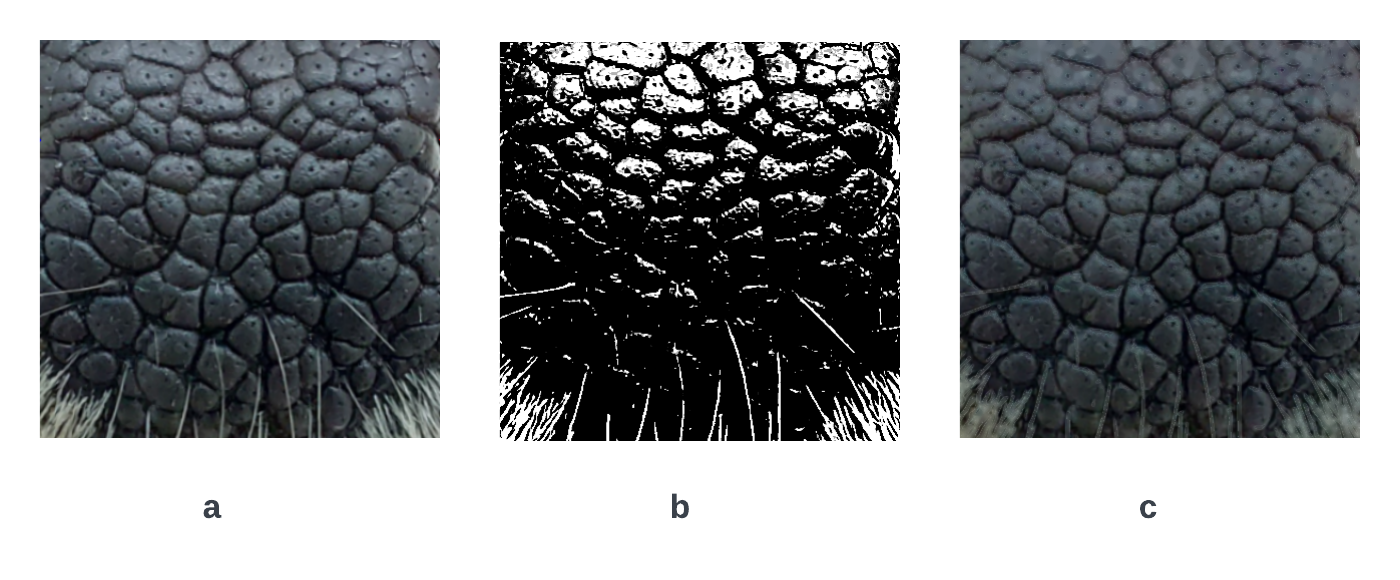
\includegraphics[width=0.9\textwidth]{obrazky/vousky.png}
	\caption{Odstranění vousků z obrazu. (a) původní obraz, (b) oblasti detekované ostřícím jádrem, (c) obraz po odstranění oblastí}
	\label{vousky}
\end{figure} 

\subsubsection{Morfologické otevření}

Dále bylo navrženo na obraz aplikovat morfologické otevření \ref{morpho_chapter} z důvodu oddělení kontur, které po binarizaci zůstaly spojeny krátkým úsekem (nejčastěji se jedná o pár pixelů v kterých se kontury dotýkají). Zároveň se díky této operaci zjemní kraje kontur, což zajistí menší paměťovou náročnost. Operaci je důležité aplikovat na obraz s malým jádrem a malým počtem iterací.V opačném případě se stane, že se deformují kontury, které byly původně v pořádku. Na následujícím obrázku je znázorněno, jak vypadají spojené kontury po aplikaci morfologického otevření \ref{rozpojeni}.

\begin{figure}[h]
	\centering
	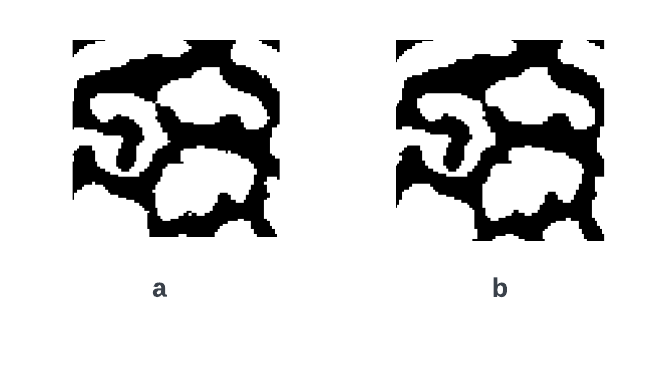
\includegraphics[width=0.8\textwidth]{obrazky/otevreni.png}
	\caption{Rozpojení dvou kontur. (a) původní obraz, (b) obraz po aplikaci morfologického otevření}
	\label{rozpojeni}
\end{figure} 

\subsubsection{Filtrace oblastí}
V této části se v obrazu opět najdou kontury. Poté se iteruje přes všechny kontury a v případě, že kontura nevyhovuje nějakému ze tří kritérií dojde k jejímu smazání. Ukázka aplikace všech kritérií současně je znázorněna na obrázku \ref{predzpracovani_navrh}.

 Prvním kritériem je velikost plochy kontury. Pro tento účel byly zvoleny pevně dvě hranice, spodní hranice o hodnotě 100 a vrchní hranice 10 000. Tyto hranice byly vybrány na základě předešlé analýzy velikostí kontur v obraze. Kontury s obsahem plochy menší než je dolní hranice u testovaných obrázků nepředstavovaly hledané polygony, ale spíše ostatní objekty. Kontury s obsahem který je větší než horní hranice reprezentovaly špatně nalezené kontury, které se sloučily dohromady. Sloučení těchto kontur se dělo hlavně z důvodu, že se na původním obrázku nacházel například příliš velký odlesk nebo vousky. Ukázka odstranění těchto částí je na obrázku \ref{filter1}.

\begin{figure}[h]
	\centering
	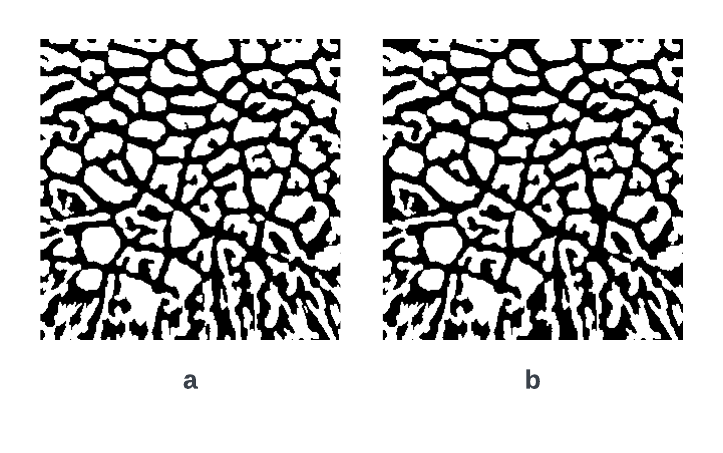
\includegraphics[width=0.6\textwidth]{obrazky/filter1.png}
	\caption{Odstranění příliš malých/velkých kontur. (a) původní obraz, (b) obraz po filtraci}
	\label{filter1}
\end{figure} 

Druhé kritérium filtrace využívá pevnosti kontury. Po testování byla zvolena hranice pevnosti na 60\%. Tato hranice se zdála jako ideální, jelikož se v obraze odstranily příliš rozbité kontury a zároveň se zachovaly kontury, které se rozpoznaly dobře. Hranice by se určitě dala navýšit, jelikož ale kontury nebývají v převážné většině případů ideálně určené, není to v aktuálním stádiu vhodné. Na obrázku níže se nachází ukázka aplikace tohoto kritéria při filtrování \ref{filter2}. 

\newpage
\begin{figure}[h]
	\centering
	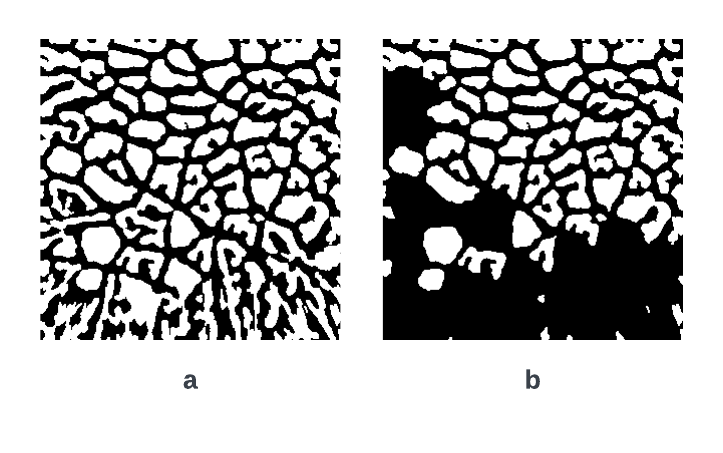
\includegraphics[width=0.6\textwidth]{obrazky/filter2.png}
	\caption{Odstranění kontur na základě pevnosti. (a) původní obraz, (b) obraz po filtraci}
	\label{filter2}
\end{figure} 

Třetí kritérium se zabývá pozicí kontury v obraze. To využívá souřadnic bodů, které kontury ohraničují. V případě, že se kontura nachází na hranici obrazu se kontura smaže. To se dělá z důvodu, že kontury na kraji nejsou v obraze celé, což by mohlo způsobit, že se v těchto konturách určí nesprávně pozice markantů (středů). Na následujícím obrázku se nachází oblast redukovaná o hraniční kontury \ref{filter3}.

\begin{figure}[h]
	\centering
	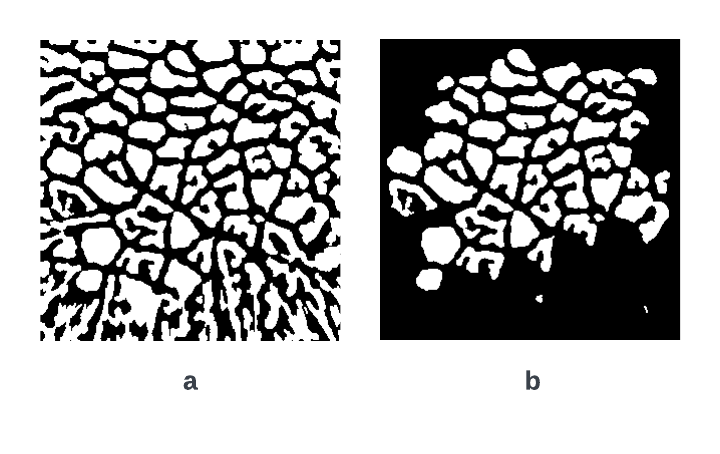
\includegraphics[width=0.6\textwidth]{obrazky/filter3.png}
	\caption{Odstranění kontur podle umístění. (a) původní obraz, (b) obraz po filtraci}
	\label{filter3}
\end{figure} 

Dalším uvažovaným kritériem pro filtraci byla velikost nalezených kontur. Myšlenkou této filtrace bylo na základě velikostí ploch kontur v obraze určit průměrnou plochu kontury a poté odstranit všechny kontury v obraze, které by se svou plochou lišili o více než zvolenou odchylku. Tento způsob se ovšem později ukázal jako neproveditelný, jelikož se rozložení velikostí ploch kontur v různých obrazech výrazně lišily a bylo obtížné tuto odchylku jednoznačně určit. Na základě zkoumání velikostí nalezených kontur při testování této myšlenky vzniklo první kritérium.


\subsection{Extrakce markantů}
Extrakce markantů je proces, který ze vstupu vygeneruje šablonu rysů. Tuto šablonu bude představovat dvoudimenzionální pole, kde v každá buňka bude reprezentovat malou oblast z původního obrazu. Například pokud má původní obraz rozměry 300x300 pixelů a pole bude mít velikost 10x10, bude každá buňka pole reprezentovat oblast o velikosti 30x30 pixelů. Následně je potřeba v obraze zjistit pozice markantů. Toho se dosáhne určením pozice středů v jednotlivých konturách pomocí jejich momentů. Poté se tyto pozice převedou do předpřipraveného pole, přičemž pozice v poli bude odpovídat původním pozicím markantů v obraze. Dále je vhodné aby velikost pole nebyla příliš velká, jelikož je nutné aby, mírná změna při anotaci nezpůsobila, že se pozice markantů připíší do jiných bloků. Na následujícím obrázku se nachází ukázka vizualizace tohoto kroku \ref{markant2pole}.


\begin{figure}[h]
	\centering
	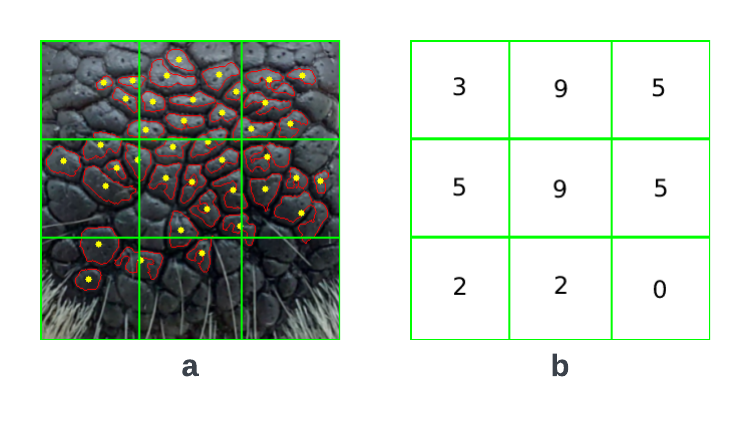
\includegraphics[width=0.6\textwidth]{obrazky/extrakce.png}
	\caption{Převod nalezených markantů na reprezentaci polem. (a) původní obraz s nalezenými markanty, (b) vizualizace pole s počtem markantů v jednotlivých buňkách}
	\label{markant2pole}
\end{figure} 

Během vývoje bylo navrženo při extrakci využít pouze pár nejvýznamnějších kontur. Toho by se dosáhlo například pomocí vybrání počtu největších kontur, z kterých by se provedla extrakce. Od této varianty bylo ale nakonec odstoupeno, jelikož se po testování ukázalo, že největší kontury většinou nebývají nejlépe určené. Na tomto nápadu se ale dále pracovalo a vzniklo z něj navržené filtrování kontur, jehož cílem je zanechat pouze ty nejlépe určené kontury.


Návrhem pro vylepšení této metody by bylo kromě pozic markantů také extrahovat jejich orientaci jako tomu bylo v práci \cite{NOVIYANTO201377}. Tímto způsobem by se měl snížil počet milných shod při porovnání, ovšem musel se změnit formát prvků v poli tak, aby kromě hodnot obsahoval i úhly korespondující k daným bodům. Jelikož se zatím jedná o první pokus o identifikaci, bude prozatím testována pouze základní varianta tohoto způsobu.


\subsection{Nalezení nejlepši shody}

Tento krok je nepovinný a záleží na uživateli, zda jej bude vyžadovat a nebo pouze skončí u výpisu extrahované šablony. Pro nalezení nejlepší shody je potřeba, aby uživatel zadal složku, v které se nachází ostatní šablony společně s fotografiemi ke kterým se šablony vážou. Navržený algoritmus poté ve vybrané složce projde všechny nalezené šablony a porovnává je s aktuálně vyextrahovanou šablonou. Po projití celé databáze se už pouze vybere šablona z databáze, s kterou se vstupní otisk shodoval nejvíce a fotografie, která k dané šabloně patří se zobrazí uživateli.




\chapter{Implementace}
Tato kapitola se věnuje implementaci návrhu, který byl prezentován v předchozí kapitole. Implementované algoritmy jsou rozděleny do dvou typů. Prvním typem jsou algoritmy, které byly převzaty z knihovny openCV. U těchto algoritmů bude provedeno porovnání konkrétních výstupů ve formě obrazů, které vznikly v závislosti na zvolených parametrech. Druhým typem jsou algoritmy, které bylo nutné navrhnout, aby bylo možné dosáhnout výsledků, které byly stanoveny v návrhu implementace. Příkladem takových algoritmů jsou rotace, změna velikosti a určení markantů. V této části budou podrobně popsány postupy, které byly použity při implementaci těchto algoritmů.

\section{Použité technologie}
Výsledný program byl implementován v jazyce Python verze 3.10.11 s pomocí několika knihoven. Stěžejní knihovnou využitou pro implementaci bylo openCV verze 4.7.0. Mezi další využité knihovny patří argparse, math a numpy. Celý program se nachází v jednom souboru a je členěn do jednotlivých funkcí. Program je možné spustit s dvěma argumenty. První argument je povinný a reprezentuje cestu ke vstupní fotografii (parametr -i/--input). Druhý nepovinný argument určuje, zda se bude vstupní fotografie porovnávat a zároveň určuje cestu ke složce v niž se nachází šablony s kterými chce uživatel vstupní fotografii porovnat (parametr -c/--cmpFile).

\subsubsection{OpenCV}
OpenCV je multiplatformní volně dostupná otevřená knihovna, která umožňuje přístup k algoritmům spojeným s počítačovým viděním. Původně byla tato knihovna vyvíjena společností intel za účelem zrychlení pokroku v oblasti rozpoznávání obrazu. Díky jeho licenci je totiž možné knihovnu využít i v komerčních aplikacích, čímž by postupně vzrostl zájem o rychlejší procesory. V dnešní době se vývoj hodně odklonil od původního intelu a do otevřeného kódu spíše přispívají jedinci, kteří knihovnu využívají. Navíc také slouží jako základní stavební kámen pro projekty spojené s počítačovým viděním a díky optimalizovanosti algoritmů není nutné vymýšlet základní operace a je možné na nich pouze stavět. Z tohoto důvodu je výsledný kód lépe čitelný a přenosný. Původně byla tato knihovna napsána v jazycích C / C++, avšak v dnešní době již podporuje i spoustu jiných jazyků jako Python a Java. Knihovna je strukturovaná do několika modulů, jako jsou například zpracovávání obrazu, detekce objektů, analýza videa a další viz \cite{opencv_doc}. V aktuální verzi openCV 4.7.0 je k dispozici přes 2500 algoritmů. Pro tuto práci bude důležitá hlavně verze openCV-Python, která slouží jako API původní knihovny openCV pro python \cite{openCV}.



\section{Načítání fotografie}

Pro načtení fotografie do programu je potřeba zadat správnou cestu k fotografii. Pokud cesta k fotografii není správná, program skončí s chybou. Načítaní se provádí v hlavní části programu pomocí funkce \texttt{imread()}.

Následně se fotografii ve fuknci \texttt{rescaleImage()} změní velikost. Vstupem do této funkce je parametr představující hodnotu nové šířky, pomocí kterého se vypočítá hodnota měřítka. Toto měřítko se poté použije pro transformaci rozměrů fotografie. Ukázka výpočtu tohoto měřítka se nachází v následující rovnici \ref{meritko_eq}. 

\begin{equation}
    \text{měřítko} = \frac{\text{šířka}_{\text{nová}}}{\text{šířka}_{\text{původní}}}
    \label{meritko_eq}
\end{equation}
Nové rozměry fotografie se poté vypočítají následovně:

\begin{equation}
    \text{šířka} = \lfloor \text{šířka}_{\text{původní}} * \text{měřítko} \rfloor
\end{equation}

\begin{equation}
    \text{výška} = \lfloor \text{výška}_{\text{původní}} * \text{měřítko} \rfloor
\end{equation}

Výsledkem toho je fotografie, která má šířku o velikosti zadané parametrem a výšku o velikosti úměrné vůči změně původní šířky fotografie. V aktuální implementaci se používá hodnota parametru 600, jelikož se jevila jako ideální velikost pro následné zobrazení uživateli. 


\subsection{Anotace fotografie}
Následně se uživateli zobrazí zvolená fotografie. Děje se tomu tak díky zavolání funkce \texttt{makeAnnotations()}. Funkce následně čeká na anotaci bodu uživatelem. Ten tak učiní pomocí dvojitého kliknutí na pixel na obrázku. Reakcí na tento klik je zavolání funkce \texttt{drawCircle()}, která na fotografii vykreslí kruh, kterým uživatele informuje o pozici výběru bodu. Následně má uživatel možnost tento bod potvrdit pomocí stisku klávesy \texttt{\textbf{a}}. V případě, že uživatel není spokojen s výběrem bodu, může pouze označit jiný bod a poté opět potvrdit výběr. Pokud by uživatel chtěl znovu vybrat již potvrzený bod, může tak učinit pomocí stisku klávesy \texttt{\textbf{r}}. Tímto celý proces začne od začátku. Po anotaci potřebných bodů už stačí pouze potvrdit výběr pomocí klávesy \texttt{\textbf{d}}. Pozice vybraných bodů jsou následně uloženy pro další postup. Důležité je při anotování brát v úvahu pořadí označení bodů. Prvně se označuje levá a poté pravá dírka.


\subsection{Rotace}
Poté je potřeba obraz převést do vhodného formátu. Toho se učiní pomocí zavolání funkce \texttt{rotateImage()}. Tato funkce má za úkol rotačně normalizovat obraz a zároveň vrací rotační matici, která se použije pro transformaci pozic anotovaných bodů.

Pro vytvoření matice rotace je potřeba zjistit úhel o který se má obrázek orotovat a bod okolo kterého se rotace provede. Souřadnice rotačního bodu jsou vypočítány jako průměr souřadnic delt. Pro výpočet úhlu bylo využito funkce \texttt{atan2()}, která je definována následovně:  

\begin{equation}
    atan2(y,x) = 
            \begin{cases}
                    \arctan (\frac{y}{x})  & \quad\text{je-li } (x > 0) \land (y >= 0),\\
                    \arctan (\frac{y}{x}) + \pi & \quad\text{je-li } (x < 0), \\
                    \arctan (\frac{y}{x}) + 2\pi & \quad\text{je-li } (x > 0) \land (y < 0), \\
                    \frac{\pi}{2}    & \quad\text{je-li } (x = 0) \land (y > 0), \\ 
                    \frac{3}{2} \pi  & \quad\text{je-li } (x = 0) \land (y < 0) \\ 
            \end{cases}
\end{equation}

Funkce řeší dva problémy, které mohou nastat při použití klasických funkcí tangens a arkustangens. Tyto problémy zahrnují dělení nulou, což může vést k hodnotám +-180, a také návratovou hodnotu, která se nachází v intervalu $(0, 360)$, zatímco klasické funkce tangens a arkustangens vrací hodnoty v intervalu $(-90, 90)$.

Pro výpočet úhlu je potřeba brát v úvahu vzájemné pozice delt, jelikož se výpočet úhlu liší v závislosti na jejich souřadnicích. Výpočet se tedy rozděluje na následující 4 případy (delta je reprezentována souřadnicemi $[x_{n}, y_{n}]$ a $x,y$ reprezentují vzálenost mezi deltami po x-ové a y-ové ose):


\begin{equation}
    \text{úhel} = 
            \begin{cases}
                    atan2(x,y) + \pi & \quad\text{je-li } (x_{1} > x_{2}) \land (y_{1} > y_{2}), \\
                    -atan2(x,y) + \pi & \quad\text{je-li } (x_{1} > x_{2}) \land (y_{1} < y_{2}), \\
                    -atan2(x,y) & \quad\text{je-li } (x_{1} < x_{2}) \land (y_{1} > y_{2}), \\
                    atan2(x,y) & \quad\text{je-li } (x_{1} < x_{2}) \land (y_{1} < y_{2}) \\ 
            \end{cases}
\end{equation}

Po zjištění bodu rotace a úhlu stačí pomocí funkce \texttt{getRotationMatrix2D()} vytvořit rotační matici. Tato matice se následně aplikuje na vstupní obraz, čímž se obraz orotuje vůči pozicím delt. 

\subsection{Získání oblasti zájmu}

Po orotování obrazu je potřeba z obrazu získat oblast zájmu. K tomu je zapotřebí získat nové souřadnice delt po rotaci pomocí funkce \texttt{getNewCoordinates()}. Tato funkce za pomocí matice použité při rotaci a funkce \texttt{transform()} určí nové souřadnice delt. 

Následně se z obrazu získá oblast zájmu. To se děje ve funkci \texttt{cropRectangle()}, která pomocí vzdálenosti mezi deltami vyřízne z obrázku čtverec představující oblast zájmu.

Nakonec už se pouze pomocí funkce \texttt{rescaleImage()} změní velikost obrazu na 300x300 pixelů. Díky těmto krokům budou všechny fotografie ve stejném formátu pro následné zpracování.

\section{Předzpracování a extrakce markantů}
Tato podkapitola se bude věnovat aplikací algoritmů z návrhu aplikace. Jelikož se většinou jedná o algoritmy, které byly již popsány dříve budou se v této části zkoumat různé parametry navržených algoritmů. V případě, že tyto algoritmy ještě nebyly pořádně vysvětleny jako třeba oprava chyb a filtrace kontur, budou náležitě popsány.

\subsection{Filtrování}
Pro filtrování obrazu se využívá bilaterálního filtrování. Tento filtr se aplikuje pomocí funkce \texttt{bilateralFilter()}. Funkce má možnost nastavení tří parametrů. První parametr představuje diametr (průměr) okolí pixelu, které se bude uvažovat pro výpočet nové hodnoty. Druhým parametrem je sigmaColor. Tento parametr reprezentuje odchylku barev, které budou brány v potaz. V případě šedotónového obrazu to jsou rozdíly intenzit. Třetím parametrem je sigmaSpace, která reprezentuje vzdálenost bodů, které budou použity pro filtrování. Na následujícím obrázku je možné vidět rozdíly mezi nastavením těchto parametrů \ref{bilateral_param}.

\begin{itemize}
    \item d = uvažované okolí pixelu
    \item $ \sigma $ = sigmaColor a sigmaSpace
\end{itemize}


\begin{figure}[h]
	\centering
	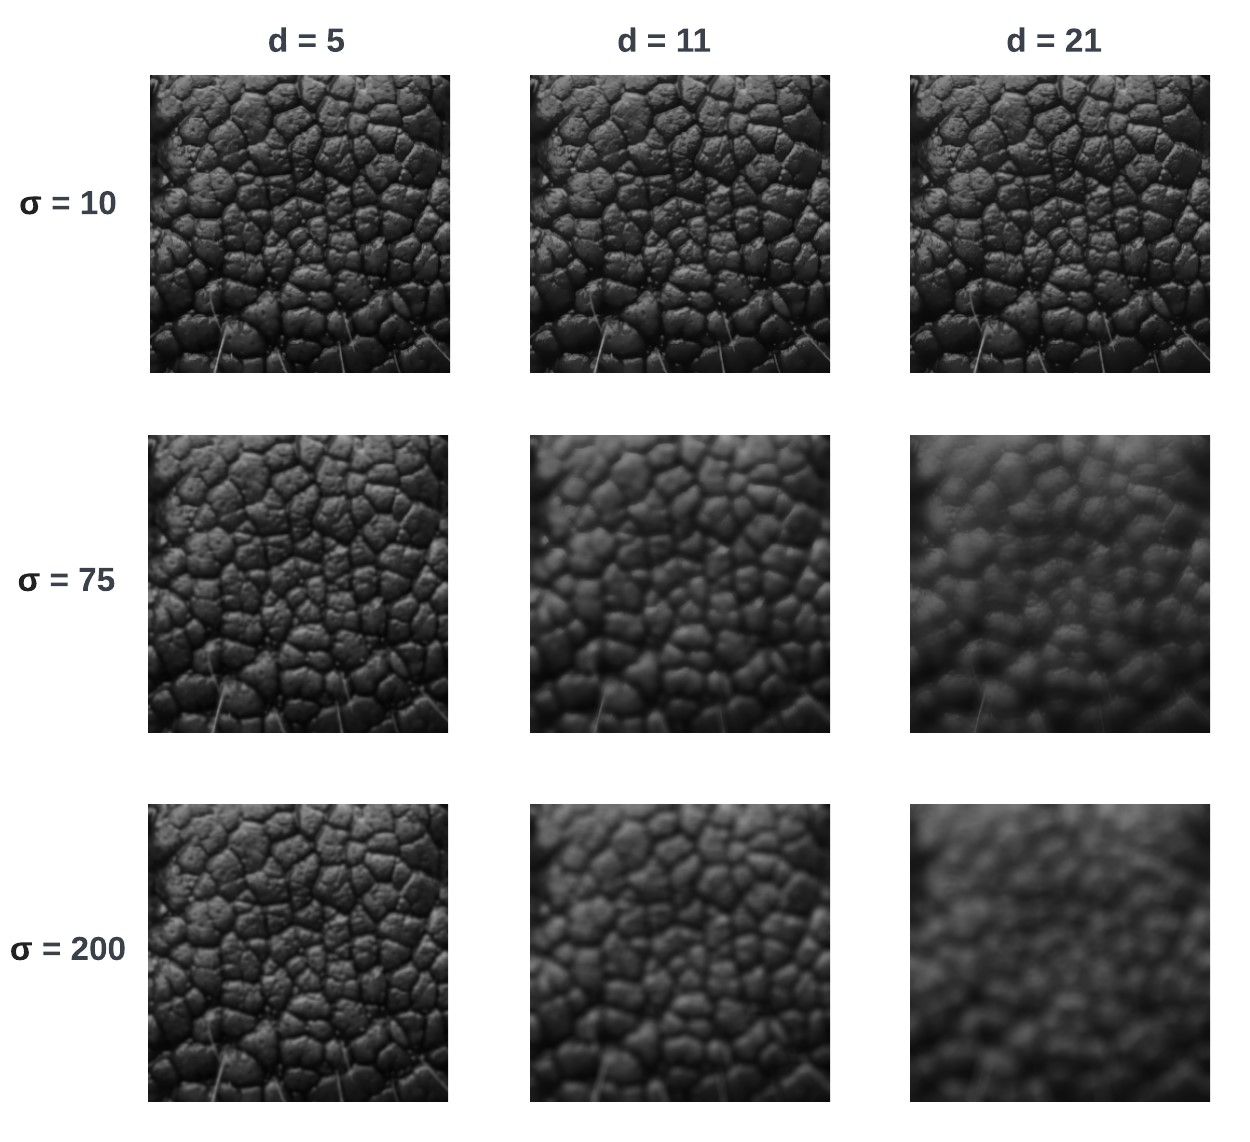
\includegraphics[width=0.9\textwidth]{obrazky/bilateral_param2.jpg}
	\caption{Použití různých parametrů bilaterálního filtru}
	\label{bilateral_param}
\end{figure} 

Z obrázku lze pozorovat, že v případě nastavení malé hodnoty diametru nebo malé hodnoty $ \sigma $, se obraz prakticky nezmění. Naopak v případě, že je diametr příliš velký, je výsledkem příliš rozmazaný obraz, v kterém je obtížné rozlišit polygon a rýhy. Na základě pozorování aplikace filtru na obrázky v databázi bylo určeno, že ideální hodnota diametru je 11 a hodnota $ \sigma $ je 75. 

\subsection{Vylepšení kontrastu}
Pro vylepšení kontrastu obrazu se používá funkce \texttt{makeClahe()}. V této funkci se pomocí dvou parametrů nastavuje proces histogramové ekvalizace. Prvním parametrem je clip-limit, kterému se již věnoval text v navržených algoritmech \ref{histo_equ}. Druhým parametrem je gridSize, který určuje, do kolika částí se obraz rozdělí. Poté se pro každou část udělá vyrovnání histogramu. Na následujícím obrázku bude ukázán vliv těchto parametrů na šedotónový obraz \ref{clahe_param}.


\begin{figure}[h]
	\centering
	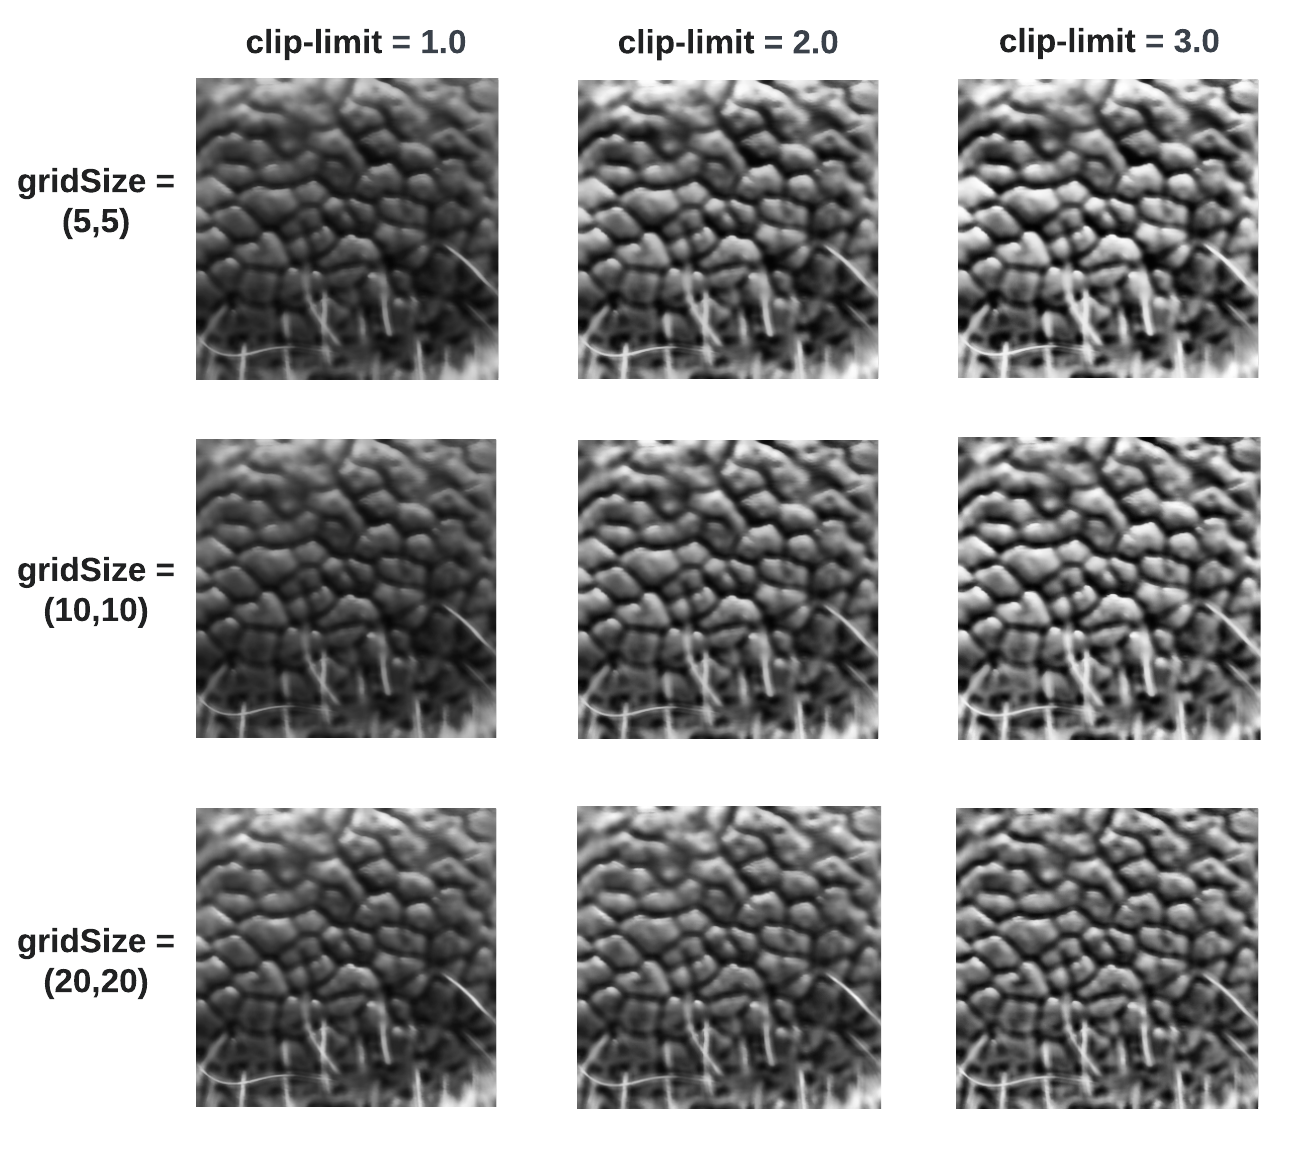
\includegraphics[width=0.9\textwidth]{obrazky/clahe_parametry.png}
	\caption{Použití různých parametrů CLAHE}
	\label{clahe_param}
\end{figure} 

Z obrázku lze vidět, že čím vyšší hodnotu clip-limit má, tím více se zvýrazňují světlé části obrazu. Nejlépe si po vizuálním testování více obrazů vedla hodnota clip-limit 2. Tato hodnota byla nejlepší, jelikož hodnota 1 měla minimální efekt na výsledný obraz a hodnota 3 až moc zvýrazňovala světlá místa na obrazu. Hodnota gridSize neměla příliš velký vliv na výsledek ekvalizace a následkem testování byla jeho hodnota určena na (10,10).


\subsection{Binarizace}
K binarizaci obrazu se používá funkce \texttt{adaptiveThreshold()}. Tato funkce má tři zajímavé parametry, které lze nastavit. Jedním z těchto parametrů je způsob pro výpočet hodnoty práhu pro daný blok. V aktuální implementaci openCV jsou dostupné dvě možnosti, průměr hodnot v bloku nebo hodnota určena váženým průměrem s Gaussovým jádrem. Pro srovnání těchto dvou způsobů bude na následujícím obrázku ukázán jejich rozdíl \ref{adaptive_kernel_diff}.

\newpage
\begin{figure}[h]
	\centering
	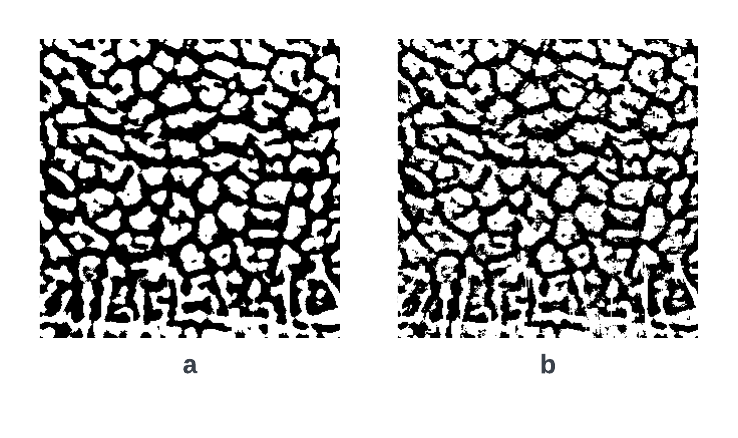
\includegraphics[width=0.9\textwidth]{obrazky/adaptive_kernels_dif.png}
	\caption{Použití různých způsobů pro určení hodnoty prahu, (a) průměr, (b) Gaussovo jádro}
	\label{adaptive_kernel_diff}
\end{figure} 

Na obrázku lze vidět, že určení prahu na základě průměru hodnot v bloku produkuje značně čistější binarizovaný obraz. Tento jev se ukazuje téměř na všech obrázcích v databázi a právě z tohoto důvodu byl způsob binarizace pomocí průměru hodnot zvolen jako ten lepší.

Dalšími dvěma nastavitelnými hodnotami při binarizaci jsou velikost bloku a také konstantní hodnota, která se odečítá od průměru nebo váženého průměru bloku. Na následujícím obrázku lze vidět rozdíly mezi použitím odlišných hodnot \ref{adaptive_kernel_diff2}.

\newpage
\begin{figure}[h]
	\centering
	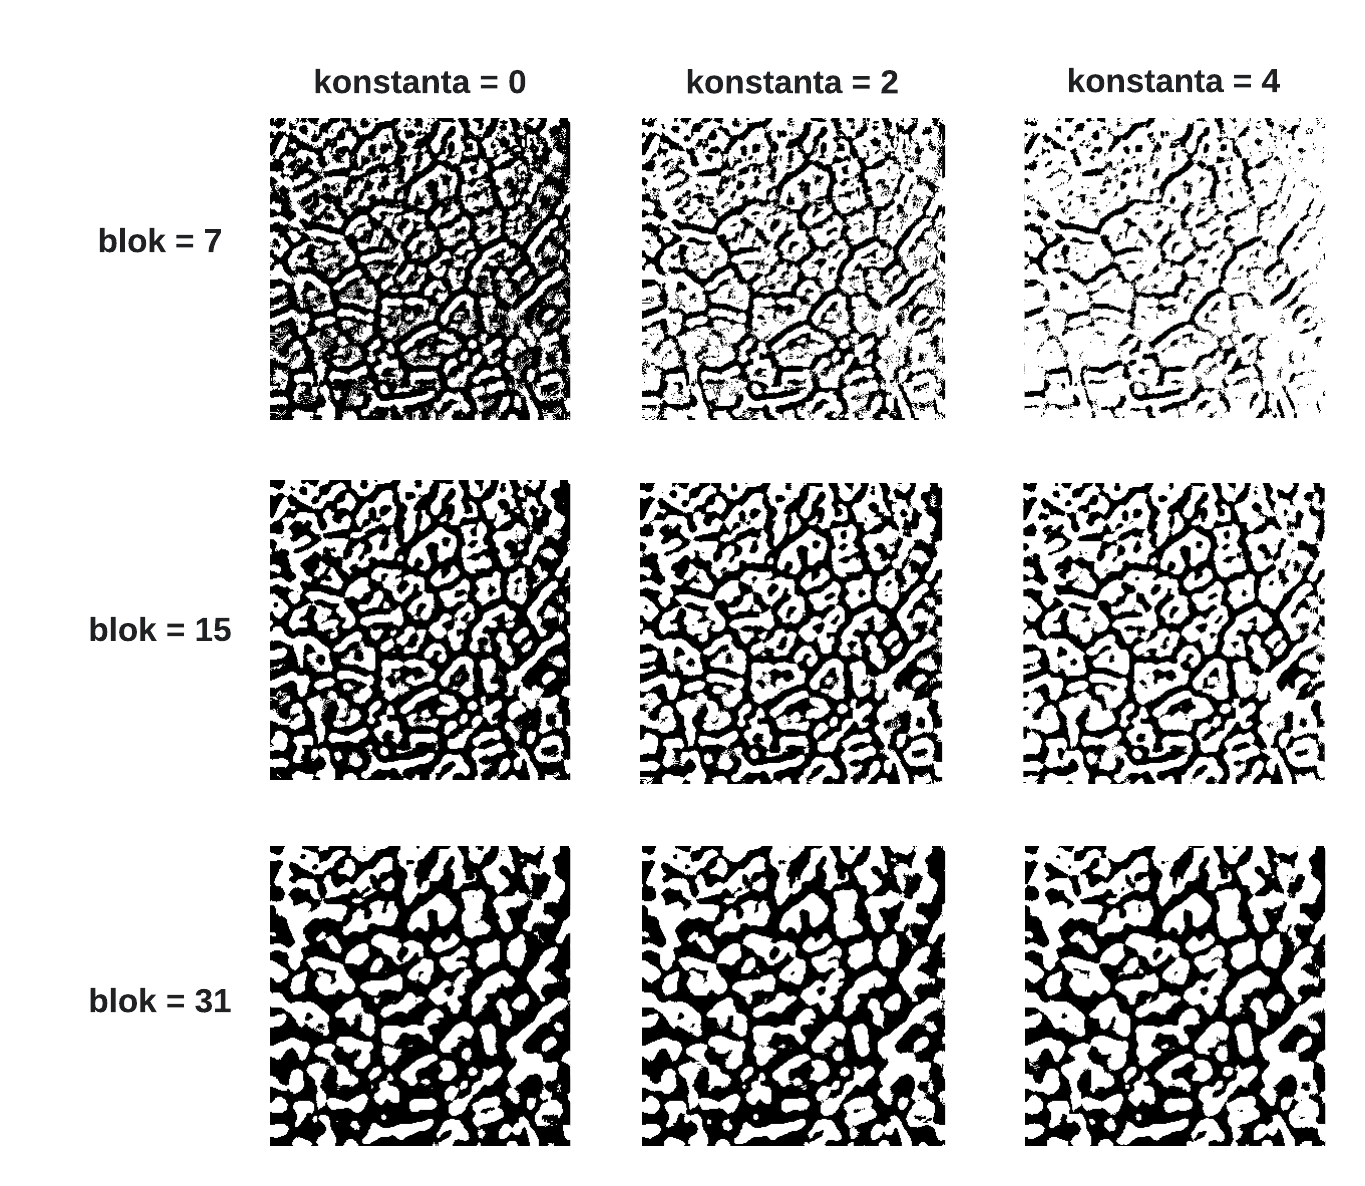
\includegraphics[width=0.9\textwidth]{obrazky/adaptive_params.png}
	\caption{Použití různých parametrů adaptivního prahování}
	\label{adaptive_kernel_diff2}
\end{figure} 

Z obrázku lze vidět, že čím větší konstanta se odečítá, tím více se pixely obarví. S rostoucí velikostí bloku klesá přesnost určení původních bloků, pokud je ale okolí příliš malé, výsledný obraz je téměř nepoužitelný. Na základě testování různých hodnot byla pro finální implementaci zvolena hodnota velikosti bloku 15 a hodnota konstanty 2. 



\subsection{Oprava chyb}

Oprava chyb formou vyplnění děravých kontur se nachází ve funkci \texttt{getFilled()}. Tato funkce si jako vstup bere binarizovaný obraz. Následně se pomocí funkce \texttt{findContours()} vrací kontury ve stromové struktuře. Poté se tato struktura prochází a u každé kontury se rozhoduje, zda se jedná o externí nebo interní konturu. Toho se dosáhne pomocí přistoupení k hierarchii na indexu 3. V případě, že je hodnota tohoto indexu záporná se jedná o venkovní konturu a tudíž se použije funkce \texttt{fillPolly()}, která v binarizovaném obraze vyplní konturu bílými pixely. Občas se stane, že tato oprava vybarví značně větší oblasti, než je vyžadováno, jelikož jsou kontury ohraničeny vousky nebo obraz není dostatečně zaostřený. Ovšem pro většinu obrazů, které jsou dobře zaostřeny a mají pěkně rozpoznatelné rozdíly mezi polygony a rýhami je tento způsob vhodný.

\subsection{Morfologické otevření}

Morfologické otevření se provádí ve funkci \texttt{getErodedDilated()}. Ve funkci se prvně vytvoří jádro pomocí funkce \texttt{getStructuringElement()} a následně se pomocí funkcí \texttt{erode()} a \texttt{dilate()} provede morfologické otevření. Mezi nastavitelné parametry v tomto procesu patří tvar strukturního elementu (jádra), jeho velikost a počet iterací aplikace dilatace a eroze. Na následujícím obrázku budou ukázány rozdíly mezi různými nastaveními počtu iterací a velikosti jádra \ref{morpho_param}. Při ukázce bylo využito kruhového strukturního elementu.


\begin{figure}[h]
	\centering
	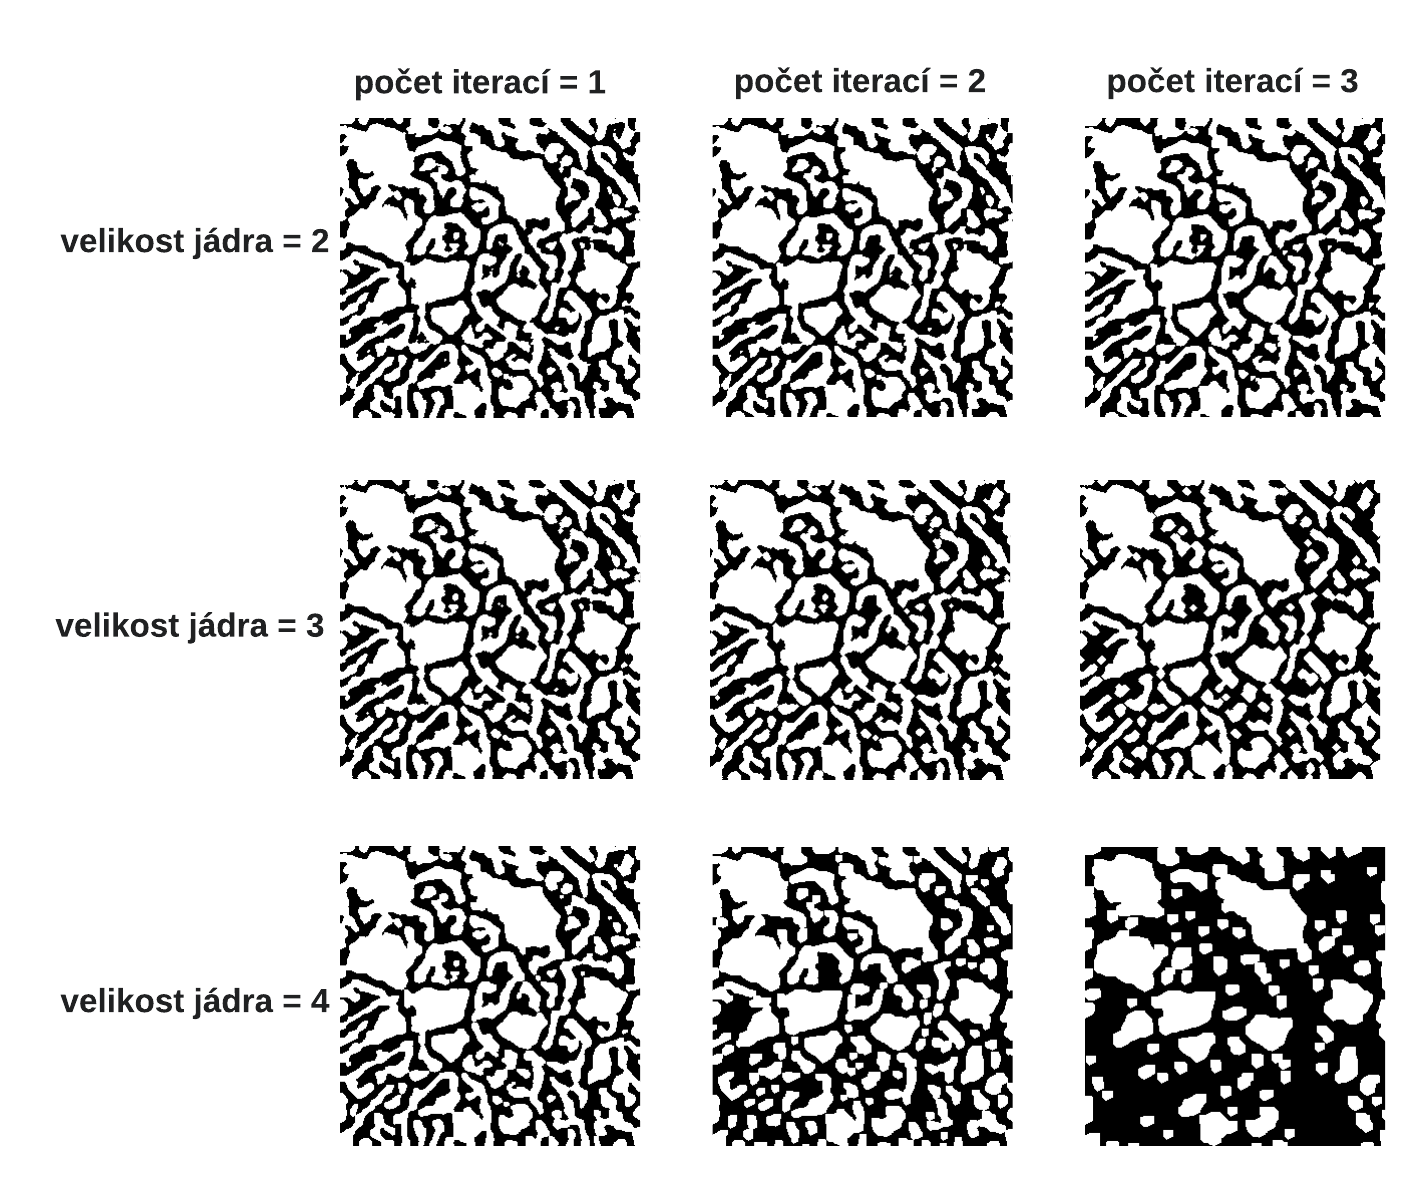
\includegraphics[width=0.9\textwidth]{obrazky/morpho_params.png}
	\caption{Použití různých parametrů morfologického otevření}
	\label{morpho_param}
\end{figure} 

Z obrázku lze vidět, že počet iterací má velký vliv na výsledný obraz, z tohoto důvodu se vyloučilo využívání více jak 2 iterací. Malá velikost jádra při nízkém počtu iterací nepřináší požadované změny do obrazu a proto také nebyla zvolena jako vhodná varianta. Dostatečně dobře se vedla velikost jádra 4 s jednou iterací, nebo také velikost jádra 2 s dvěma iteracemi. Po delším pozorování se ukázalo, že si s rušením malých spojů a zároveň zachováním původních tvarů vedla varianta s velikostí jádra 4 a jednou iterací.  

Co se týče tvaru strukturního elementu byl zvolen právě výše uvedený kruh. Při použití jiných útvarů byly vzhledem k malému počtu iterací a malé velikosti jádra pouze zanedbatelné rozdíly.


\subsection{Filtrace kontur}

Filtrace kontur se nachází ve funkci \texttt{getFiltered()}. Tato funkce vezme vstupní obrázek a poté pomocí funkce \texttt{findContours()} vyhledá kontury, které se uloží ve formě seznamu. Poté se tímto seznamem postupně prochází kontury a testuje se, zda kontura vyhovuje kritériím. 

První kritérium velikosti využívá funkce \texttt{contourArea()} a kontroluje, zda tato funkce vrací hodnotu mezi 100 a 10 000.

Druhé kritérium týkající se Huulovy aproximace využívá funkce \texttt{convexHuul()} pro převedení kontury do její konvexní podoby. Poté se pomocí funkce \texttt{contourArea()} ověří, že obsah plochy původní kontury není menší než 60\% obsahu plochy konvexní kontury.

Třetí kritérium využívá funkce \texttt{boundingRect()}, která kolem kontury udělá ohraničující čtyřúhelník. Tato funkce vrací x-ovou a y-ovou souřadnici společně s výškou a šířkou ohraničujícího okna. Poté se pouze kontroluje zda se některý z vrcholů čtyřúhelníku nenachází na okraji obrazu. 


\subsection{Extrakce markantů}

Extrakce markantů se nachází ve funkci \texttt{getCentroids()}. Ve funkci se opět najdou kontury, které se postupně prochází. Pro každou konturu se funkcí \texttt{moments()} získají momenty kontury. Následně se pomocí vzorce \ref{centroid_eq} získá střed kontury, který se poté uloží do předpřipraveného pole. Kromě ukládání pozic středů kontur (markantů) se zde také pomocí funkcí \texttt{drawContours()} a \texttt{cirlce()} vykreslují pozice markantů a kontur do původní fotografie. Výstupem funkce je poté obraz se znázorněnými konturami a markanty a také pole, v kterém jsou uloženy pozice markantů.

Jelikož jsou tyto pozice reprezentovány x-ovými a y-ovými souřadnicemi, nejsou vhodné pro další postup. Z tohoto důvodu se zavolá funkce \texttt{getPositionArray()}, která převede původní list na upravený list, který byl uveden v návrhu. Upravený list použitý v implementaci má rozměry 30x30.



\section{Porovnávání šablon a export informací}
V případě, že uživatel zvolil možnost s porovnáváním se zavolá funkce \texttt{findBestMatch()}. V této funkci se poté otevře složka zadaná v argumentu při spouštění. V této složce se poté prochází všechny soubory a v případě, že soubor je v textovém formátu (jedná se o šablonu) se obsah tohoto souboru uloží do listu. Tento list se poté převede do stejného formátu jako je list s markanty nalezenými při extrakci. Poté se zavolá funkce \texttt{comapreArray()}, která tyto dvě pole porovnává.

%\subsection{Porovnávání šablon}
Porovnávání je implementováno pomocí průchodu přes každou buňku obou listů. V každé buňce se do proměnné uchovávající celkový počet markantů přičte maximum z hodnot listů v aktuální buňce. Kromě toho se zde také do druhé proměnné představující shodný počet markantů v aktuální buňce přičítá minimum z hodnot.

Tyto hodnoty se poté vrací do původní funkce, kde se vypočítá procentuální shodnost dvou šablon. Pokud se jedná o dosavadně nejvyšší hodnotu, uloží se společně s názvem souboru, který dosáhl nejlepší shody.

Po dokončení procházení všech souborů funkce vrátí cestu k fotografii s nejlepší shodou společně s procentuální shodností. Nakonec se v hlavní části programu pomocí funkce \texttt{imshow()} zobrazí fotografie, s kterou se vstupní nejvíce shodovala společně se vstupní fotografií. V popisu zobrazené fotografie se nachází vypočítaná shodnost a název této fotografie.

%\subsection{Export informací}
V případě, že si uživatel nezvolil možnost s porovnáváním se pouze vypíše vyextrahovaná šablona v textovém formátu na standardní výstup.


\chapter{Testování a vyhodnocení}
Tato kapitola se zaměřuje na posouzení implementovaného postupu pro extrakci markantů. V její úvodní části je uveden obecný popis databáze a způsob jejího vytvoření. Dále je zde popsán postup, pomocí kterého se určovala správnost extrakce markantů, včetně nejčastějších problémů, které se při extrakci vyskytovaly. V této části jsou rovněž prezentovány grafy, které vizualizují přesnost implementovaného přístupu. Nakonec je zde uveden stručný text, v němž je popsána problematika implementovaného algoritmu pro nalezení nejlepší shody (rozpoznávání).

\section{Databáze}
Databáze je tvořena množinou dvojic souborů. Tyto dvojice jsou od sebe odlišitelné názvem a jsou tvořeny fotografií nosu a šablonou s markanty v textové podobě. Při vytváření databáze bylo využito tří separátních programů z důvodu lepšího hromadného zpracování. Jeden z těchto programů sloužil k hromadné anotaci fotek a fungoval stejně jako funkce pro anotaci ve finální verzi programu s výjimkou toho, že označené body se neukládaly do proměnné ale do souboru. Následně byly tyto body načteny druhým programem a ten na základě zadaných bodů vyřízl oblast zájmu. Třetí program poté aplikoval stejnou posloupnost operací jako byly popsány v implementaci. Výsledky extrakce byly poté uloženy do šablony se stejným názvem jako původní fotografie. Celkově se v této databázi nachází 171 fotografií. 

\section{Přesnost extrakce markantů}

Ještě před samotným určením přesnosti extrakce je potřeba vědět, jakým způsobem se tato přesnost určovala.

Přesnost byla definována jako počet správně určených marakntů vůči celkovému počtu extrahovaných marakntů. Aby bylo možné určit, co je špatný a co dobrý výsledek určení markantu, bylo potřeba projít všechny výsledky extrakce a v těch ručně vyznačit, zda se jedná o správně určený markant či nikoli.

Správnost tohoto určení se dělala na základě vizuální kontroly. V případě že pozice markantu odpovídala středu polygonu, bylo určení považováno za správné. Pokud nebylo z fotografie zcela zřejmé, zda se markant správně identifikoval, rozhodnutí bylo nakloněno k výsledku, který byl stanoven pomocí aplikovaného algoritmu.


Mezi nejčastějšími problémy při určovování markantů se vyskytovaly následující:

\begin{itemize}
    \item Rozdělení kontury do dvou, což způsobilo určení dvou markantů místo jednoho viz \ref{chyby_v_exktrakci} (a)
    \item Určení markantů v místech, kde se nacházelo ochlupení viz \ref{chyby_v_exktrakci} (b)
    \item Určení pozice markantu ve středu oblasti odlesku místo středu polygonu viz \ref{chyby_v_exktrakci} (c)
    \item Určení markantu v konturách na okraji obrazu (tyto kontury by měly být odstraněny pomocí implementovaného filtru) viz \ref{chyby_v_exktrakci} (d)
\end{itemize}


\begin{figure}[h]
	\centering
	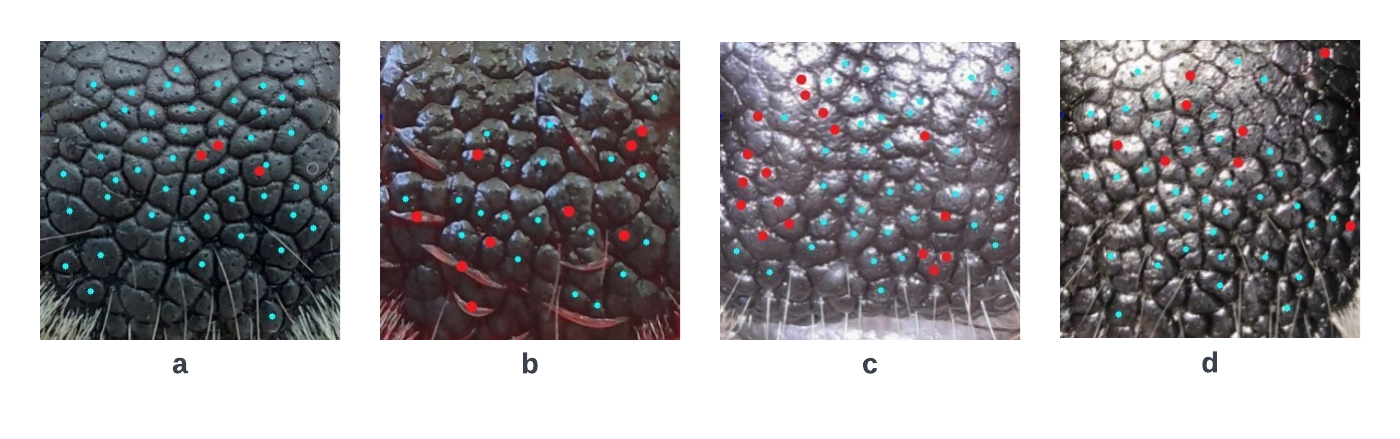
\includegraphics[width=1\textwidth]{obrazky/chyby_v_exktrakci.png}
	\caption{Nejčastější problémy při určování markantů. Červeně jsou označeny špatně určené markanty. Modře jsou označeny správně určené markanty.}
	\label{chyby_v_exktrakci}
\end{figure} 


Na grafu \ref{graph1} je možné vidět fotografie rozdělené do skupin podle počtu extrahovaných markantů. Z tohoto grafu vyčíst, že průměrný počet extrahovaných markantů činí zhruba 40 markantů. 


\begin{figure}[h]
	\centering
	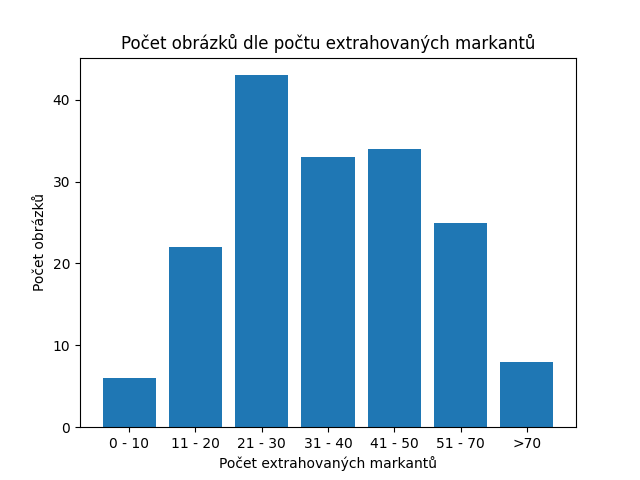
\includegraphics[width=0.7\textwidth]{obrazky/graph1.png}
	\caption{Graf reprezentující určení markantů}
	\label{graph1}
\end{figure} 

Fotografie byly poté rozděleny do skupin podle počtu extrahovaných markantů jako je znázorněno na grafu výše. Pro tyto skupiny byla následně určena úspěšnost extrakce, která se vypočítala jako celkový počet úspěšně určených markantů ve skupině fotografií podělena celkovým počtem markantů ve skupině.

Výsledky pro jednotlivé skupiny byly následující:

\begin{equation}
    \text{Přesnost} = 
            \begin{cases}
                    85.1\% & \quad\text{počet markantů}  \in (0,10\rangle \\
                    78.96\% & \quad\text{počet markantů} \in (11,20\rangle \\
                    79.42\% & \quad\text{počet markantů} \in (21,30\rangle \\
                    85.45\% & \quad\text{počet markantů} \in (31,40\rangle \\ 
                    82.35\% & \quad\text{počet markantů}  \in (41,50\rangle \\ 
                    82.32\% & \quad\text{počet markantů}  \in (51,70\rangle \\ 
                    87.33\% & \quad\text{počet markantů}  \in (70, \infty)
            \end{cases}
\end{equation}

\textbf{Celková přesnost extrakce} byla poté vypočítána stejně jako úspěšnost extrakce jednotlivých skupin a činila 82,71\%.

\subsubsection{Souvislost chybovosti na počtu extrahovaných markantů}

Pro další testování byly vstupní fotografie seřazeny podle počtu extrahovaných markantů. Následně byl celkový objem fotografií nevzorkován, aby byl výsledný graf lépe čitelný.


\begin{figure}[h]
	\centering
	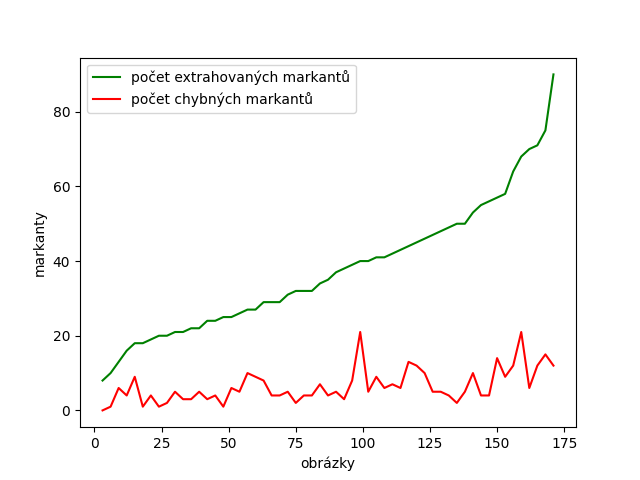
\includegraphics[width=0.65\textwidth]{obrazky/graph2.png}
	\caption{Graf reprezentující souvislost chybovosti na počtu extrahovaných markantů}
	\label{graph2}
\end{figure} 

Z grafu \ref{graph2} lze vyčíst, že počet chyb v obrázku nijak nesouvisí s počtem extrahovaných markantů. Chyby se vyskytují náhodně a jsou způsobeny ostatními vlivy zmíněnými dříve.

\section{Úspěšnost rozpoznávání}
Pokud jde o úspěšnost rozpoznávání, stanovení konkrétního procentuálního úspěchu je velmi obtížné, protože zarovnání šablony závisí na deltách, které jsou určeny manuální anotací uživatelem. To znamená, že se nalezené markanty mohou nacházet na různých místech. Z tohoto důvodu by bylo vhodné pro porovnávání dvou šablon s markanty prozkoumat další metody, které by mohly vést k lepším výsledkům.


\chapter{Závěr}

Tato bakalářská práce měla za úkol vytvořit aplikaci pro zpracování obrazu a extrakci vlastností za účelem vyhledávání markantů pro identifikaci zvěře. Vzhledem k tomu, že se jednalo o první práci tohoto druhu, byla tato problematika zkoumána pouze na nosech zvěře typu jelen a srnka.

Pro vytvoření zmíněné aplikace bylo nutné se seznámit s oborem biometrie a oblastí zaměřenou na rozpoznávání lidí na základě otisků prstů. Studované práce měly hlavní přínos v podobě rozpoznávání na základě markantů, avšak tento způsob bylo nutné upravit, aby odpovídal odlišné biometrické charakteristice, konkrétně vzoru nosu. Z tohoto důvodu bylo nutné seznámit se s touto charakterisitkou a s různými problémy, které s ní souvisejí. Na základě podobnosti se strukurou otisku prstu bylo určeno, že vhodnou pozicí pro maraknty budou středy uzavřených oblastí na vzoru nosu. Nicméně, dalším vhodným způsobem pro určení markantů by mohly být útvary rýh, které tyto oblasti ohraničují. K navržení postupu získání markantů bylo potřeba prostudovat i další práce, které se zabývají identifikací zvěře, konkrétně dobytka a psů. Hlavním přínosem těchto prací byla myšlenka získání oblasti zájmu, která z původní fotografie odstranila nepotřebné části. Jelikož tyto práce využívaly obecných přístupů pro vyhledání identifikačních bodů na fotografiích nosu, byl z těchto prací vytvořen souhrn, který by mohl posloužit jako základ pro navazující práce. 

Ve finální verzi tohoto přístupu se využilo již zmíněného získání oblasti zájmu. Na oblast se poté aplikovala řada algoritmů, které měly za cíl převést obraz do podoby vhodné pro extrakci rysů. K tomu bylo potřeba obraz převést na šedotónovou variantu, na kterou se následně aplikoval bilaterální filtr, který z obrazu odstranil nežádoucí šum a zároveň zanechal kontrast mezi přechody rýh a uzavřených oblastí. Poté bylo na obraz aplikováno CLAHE, které zvýšilo kontrast mezi zmíněnými přechody. Následně se obraz binarizoval a pomocí oprav, morfologického otevření a filtrace kontur se převedl do požadované podoby. Markanty se vyhledaly pomocí určení středů zbývajících kontur. Následně v závislosti na vstupu od uživatele bylo možné tyto pozice převést do šablon a vypsat, nebo provést porovnávání.

Na konci bylo provedeno testování s cílem určit přesnost extrakce markantů. Při využití databáze o velikosti 171 fotografií, které byly pořízeny za různých podmínek, bylo dosaženo přesnosti 82,71\%.

Z výše uvedených bodů je zřejmé, že byly splněny všechny požadavky stanovené v zadání. Navíc bylo v této práci implementováno rozšíření, které se zaměřuje na porovnání šablon a nalezení nejpodobnější fotografie. Dalším rozšířením tohoto přístupu by bylo extrahování orientace markantů, což by vedlo k ještě přesnějšímu porovnávání.


%===============================================================================

% Pro kompilaci po částech (viz projekt.tex) nutno odkomentovat
%\end{document}

  \fi
  
  % Kompilace po částech (viz výše, nutno odkomentovat a zakomentovat input výše)
  % Compilation piecewise (see above, it is necessary to uncomment it and comment out input above)
  %\subfile{chapters/projekt-01-uvod-introduction}
  % ...
  %\subfile{chapters/projekt-05-zaver-conclusion}

  % Pouzita literatura / Bibliography
  % ----------------------------------------------
\ifslovak
  \makeatletter
  \def\@openbib@code{\addcontentsline{toc}{chapter}{Literatúra}}
  \makeatother
  \bibliographystyle{bib-styles/Pysny/skplain}
\else
  \ifczech
    \makeatletter
    \def\@openbib@code{\addcontentsline{toc}{chapter}{Literatura}}
    \makeatother
    \bibliographystyle{bib-styles/Pysny/czplain}
  \else 
    \makeatletter
    \def\@openbib@code{\addcontentsline{toc}{chapter}{Bibliography}}
    \makeatother
    \bibliographystyle{bib-styles/Pysny/enplain}
  %  \bibliographystyle{alpha}
  \fi
\fi
  \begin{flushleft}
  \bibliography{projekt-20-literatura-bibliography}
  \end{flushleft}

  % vynechani stranky v oboustrannem rezimu
  % Skip the page in the two-sided mode
  \iftwoside
    \cleardoublepage
  \fi

  % Prilohy / Appendices
  % ---------------------------------------------
  \appendix
\ifczech
  \renewcommand{\appendixpagename}{Přílohy}
  \renewcommand{\appendixtocname}{Přílohy}
  \renewcommand{\appendixname}{Příloha}
\fi
\ifslovak
  \renewcommand{\appendixpagename}{Prílohy}
  \renewcommand{\appendixtocname}{Prílohy}
  \renewcommand{\appendixname}{Príloha}
\fi
%  \appendixpage

% vynechani stranky v oboustrannem rezimu
% Skip the page in the two-sided mode
%\iftwoside
%  \cleardoublepage
%\fi
  
\ifslovak
%  \section*{Zoznam príloh}
%  \addcontentsline{toc}{section}{Zoznam príloh}
\else
  \ifczech
%    \section*{Seznam příloh}
%    \addcontentsline{toc}{section}{Seznam příloh}
  \else
%    \section*{List of Appendices}
%    \addcontentsline{toc}{section}{List of Appendices}
  \fi
\fi
  \startcontents[chapters]
  \setlength{\parskip}{0pt} 
  % seznam příloh / list of appendices
  % \printcontents[chapters]{l}{0}{\setcounter{tocdepth}{2}}
  
  \ifODSAZ
    \setlength{\parskip}{0.5\bigskipamount}
  \else
    \setlength{\parskip}{0pt}
  \fi
  
  % vynechani stranky v oboustrannem rezimu
  \iftwoside
    \cleardoublepage
  \fi
  
  % Přílohy / Appendices
  \ifenglish
    \input{projekt-30-prilohy-appendices-en}
  \else
    % Tento soubor nahraďte vlastním souborem s přílohami (nadpisy níže jsou pouze pro příklad)

% Pro kompilaci po částech (viz projekt.tex), nutno odkomentovat a upravit
%\documentclass[../projekt.tex]{subfiles}
%\begin{document}

% Umístění obsahu paměťového média do příloh je vhodné konzultovat s vedoucím
%\chapter{Obsah přiloženého paměťového média}

%\chapter{Manuál}

%\chapter{Konfigurační soubor}

%\chapter{RelaxNG Schéma konfiguračního souboru}

%\chapter{Plakát}

% Pro kompilaci po částech (viz projekt.tex) nutno odkomentovat
%\end{document}

  \fi
  
  % Kompilace po částech (viz výše, nutno odkomentovat)
  % Compilation piecewise (see above, it is necessary to uncomment it)
  %\subfile{projekt-30-prilohy-appendices}
  
\end{document}
